\documentclass[12pt]{article}

\usepackage{float}
\usepackage{fancyhdr}
\usepackage{amsmath}
\usepackage{amsthm}
\usepackage{mathrsfs}
\usepackage{graphicx}
\usepackage{graphics}
\usepackage{subcaption}
\usepackage{hyperref}
\usepackage{wrapfig}
\usepackage{arydshln}
\usepackage{multirow} 
\usepackage{appendix}
\usepackage{pythonhighlight}
\usepackage{tikz}

\usepackage[natbib=true,
    style=numeric,
    sorting=none]{biblatex}
\addbibresource{bibi.bib}

\begin{document}
\begin{titlepage}
	\centering
	{\textsc{University of Bonn} \par}
	\vspace{1cm}
	{\Large \textsc{Lab report}\par}
	\vspace{1.5cm}
	{\huge\bfseries  Photometry of star clusters\par}
	\vspace{2cm}
	{\Large\itshape Wajdee Chayeb \\
	MohammadReza Torkamani\par}
	\vfill
	Tutors:\par
	Rupal Giri\\
	Aditya Pandya\\
        Gervit Kumar Trehan

	\vfill

% Bottom of the page
	{\large \today\par}
\end{titlepage}

\tableofcontents


\section{Introduction}
A star cluster is a gravitationally bound system of stars that originates from the collapse of a single molecular cloud \cite{lecturenote}. They are the fundamental building blocks of galaxies since nearly all stars have once been members of a cluster and also play a key role in understanding the stellar evolution theories \cite{lecturenote}. 
Star clusters are known to be in two types, open and globular, where the first has lower mass range, size and density. and the latter is older more massive, and bigger in size \cite{lecturenote}. Here comes the importance of studying globular clusters as their age put a strong limit on the determination of the age of the whole universe. 
To investigate the main properties of a cluster (distance, age, and color), one would need to construct a color magnitude diagram (CMD). This CMD is a correlation between the absolute magnitude of the stars forming a cluster and their corresponding temperatures in terms of a color index \cite{lecturenote}. 
In this work, we construct a CMD of the open cluster M34 using a photometric observation, taking images in different bands of color. This is done using a 50 cm optical Cassegrain telescope on the rooftop at the Argelander-Institut fur Astronomie at the University of Bonn. Multiple image processing steps are done to get information from raw data needed to construct the CMD and determine the main characteristics of the cluster.  

\section{Data Reduction \& Image Processing}

\subsection{Bias Subtraction}
A received analog signal at the CCD camera is digitized using an analog to digital converter (ADC) where each pixel is assigned a number between 0 and $2^{n}$, where n is the number of bits in the ADC. To ensure that the ADC always receives a positive signal, an electronic offset is added for each pixel to make sure that the CCD chip works in the linear regime and also to avoid having small voltages causing negative values \cite{lecturenote}. Thus, we start the data reduction by subtracting the bias. which is done by first taking the mean of all bias frames using numpy.mean in Python. this defines a MASTER BIAS frame, shown in Figure \ref{fig1}. Then, we subtract the MASTER BIAS frame from every individual frame.  

\begin{figure}[H]
    \centering
    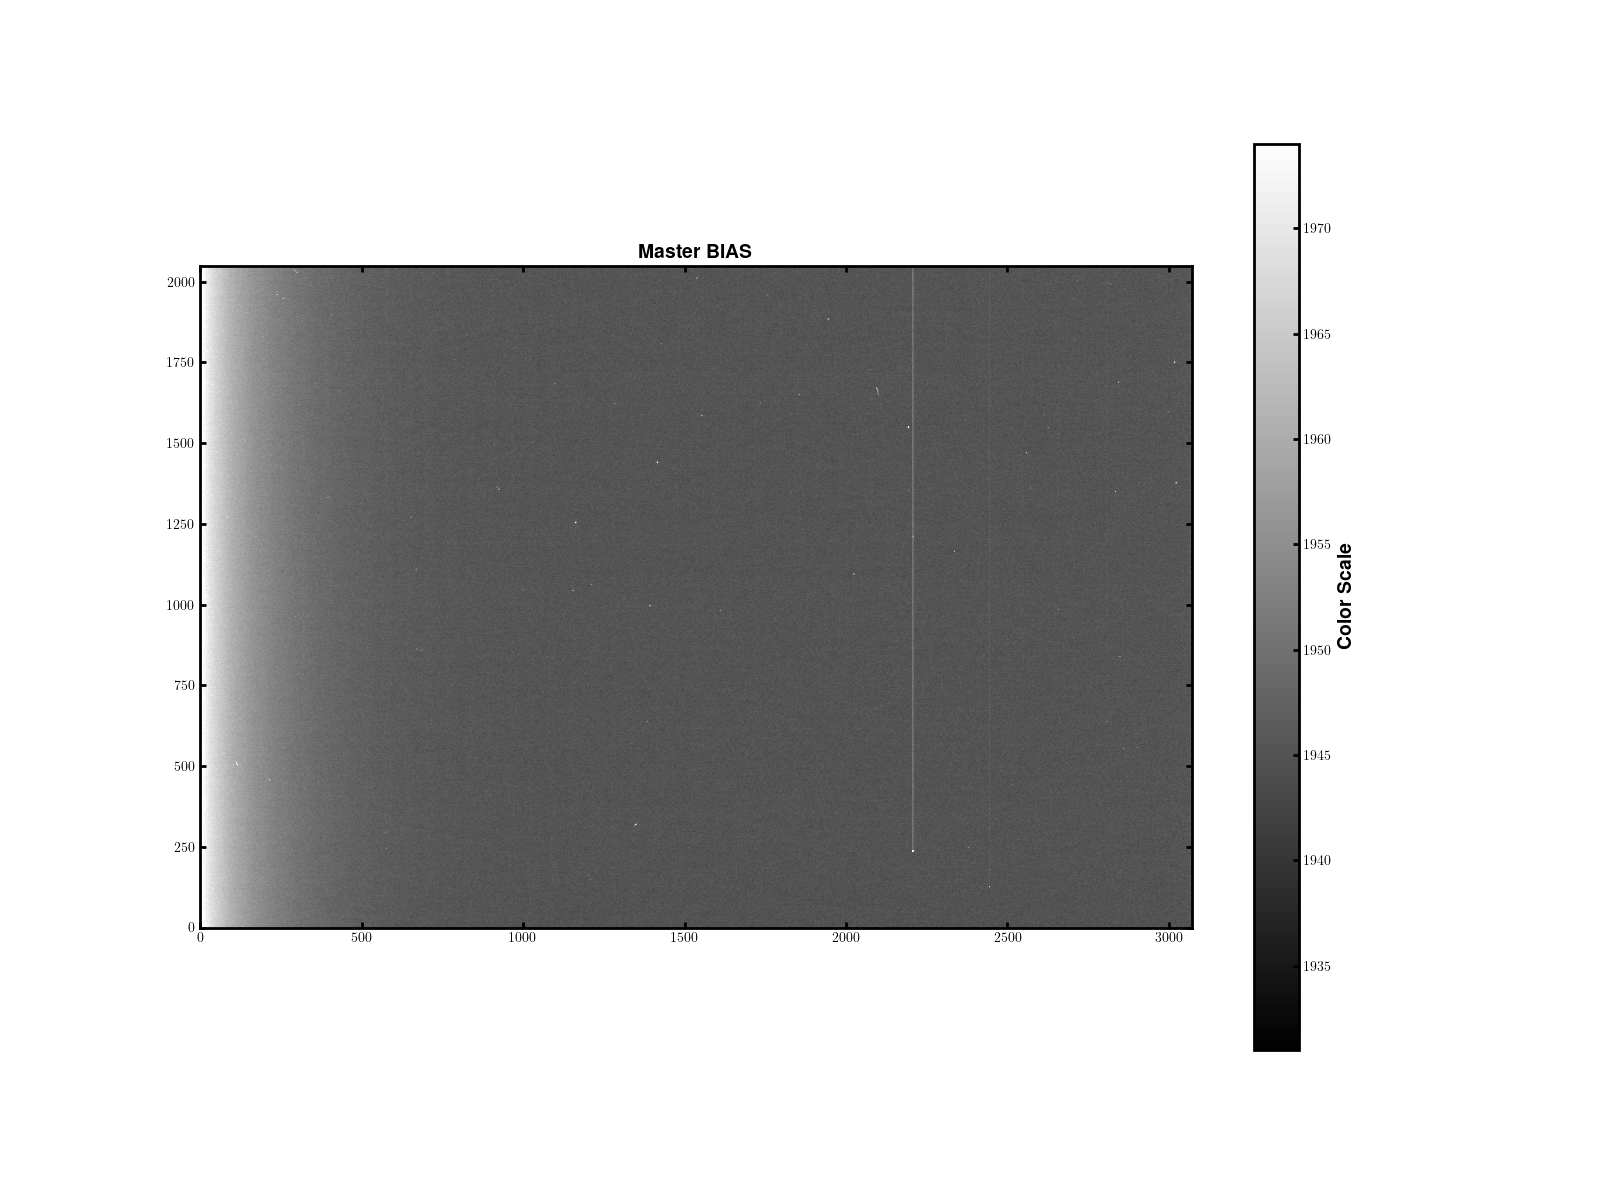
\includegraphics[width=\textwidth]{fig/Master_BIAS.png}
    
    \caption{MASTER BIAS Frame shown in limited linear scale}
    \label{fig1}
    \end{figure}
    


\subsection{Dark Subtraction}
Another source of noise when there is no light exposure is the dark current, which arises due to thermal fluctuations \cite{lecturenote}. A current flows in the CCD chip appearing in every pixel. Different dark currents in the pixels across the CCD result in a fixed pattern of noise, a mean of which can be removed by taking DARK frames and subtracting them from the science and FLAT frames. Thus, we take the mean of the dark frames resulting in a MASTER DARK frame, shown in Fig \ref{fig2}, which we subtract from the science and FLAT frames regarding to their exposure time, for instance it is directly subtracted from science frames however when it comes to FLAT frames a factor $\dfrac{t_{flat}}{t_{dark}}$ is needed. when $t_{flat}$ is the exposure time in FLAT frames and $t_{dartk}$ is the exposure time in DARK frames. Since the dark current arises from thermal motions, one can reduce it by cooling the CCD thermoelectrically \cite{lecturenote}. 

\begin{figure}[H]
    \centering
    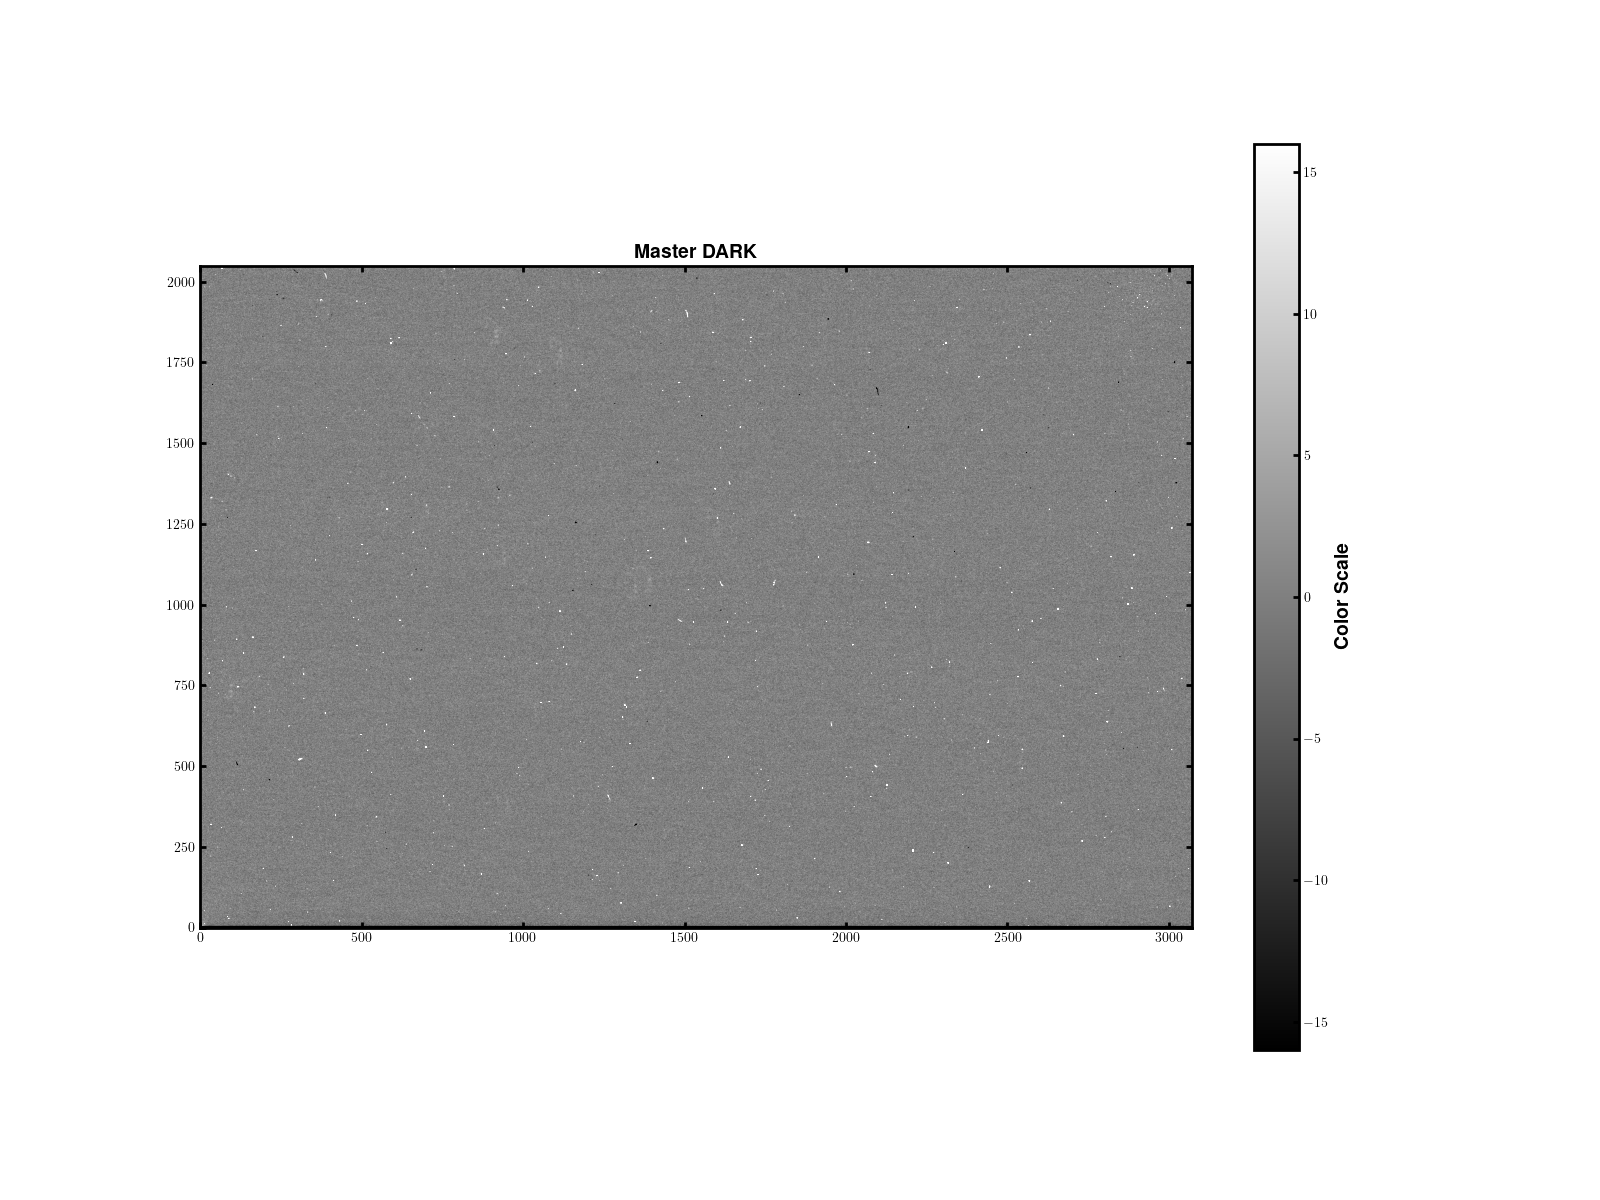
\includegraphics[width=\textwidth]{fig/Master_DARK.png}
    \caption{MASTER DARK Frame, shown in limited linear scale}
      \label{fig2}
    \end{figure}
    
\subsection{Flat Fields}
Some FLAT frames are taken by making an exposure toward a uniformly illuminated dome flat field screen. We expect to see in the FLAT frames variations of light as well as dust grains within the light path presented as donuts \cite{lecturenote}. Therefore, by flat fielding, we can correct the CCD output at each pixel so that the pixels respond evenly to a source with identical photon flux. To proceed in data analysis, we take the average of FLAT frames \ref{master_flat} and normalize it to an average value of 1 \ref{normal_master_flat}. Then, Each science frame is generated by subtracting the master dark frame and the master bias frame (which has already been subtracted in the initial step of image reduction), and then dividing the result by the normalized flat frame. Since the response of pixels is wavelength-dependent, we evaluate the data using three different filters B, R, and V. We will restrict the visualization of our results in this report to filter B and show the rest in the Appendix. \ref{append}

\begin{figure}[H]
    \centering
    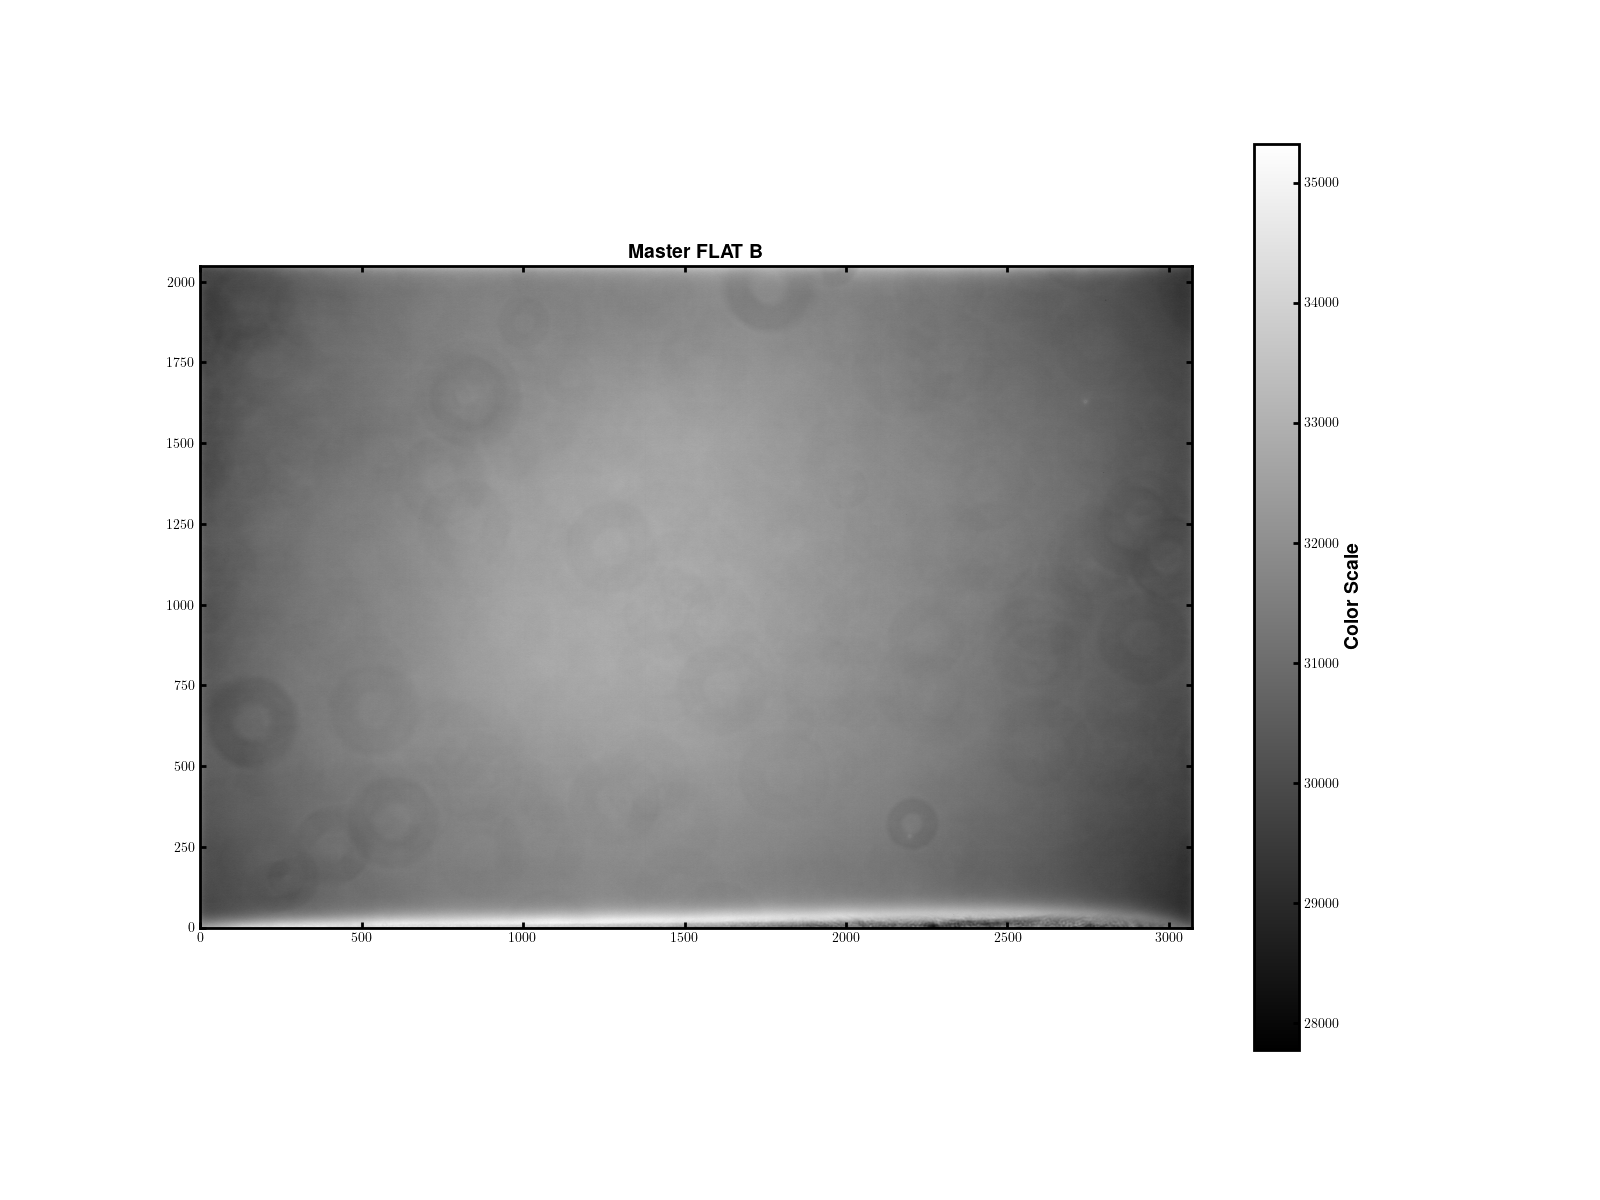
\includegraphics[width=\textwidth]{fig/Master_FLAT_B.png}
    \caption{MASTER FLAT frame in the B band}
    \label{master_flat}
\end{figure}


\begin{figure}[H]
    \centering
    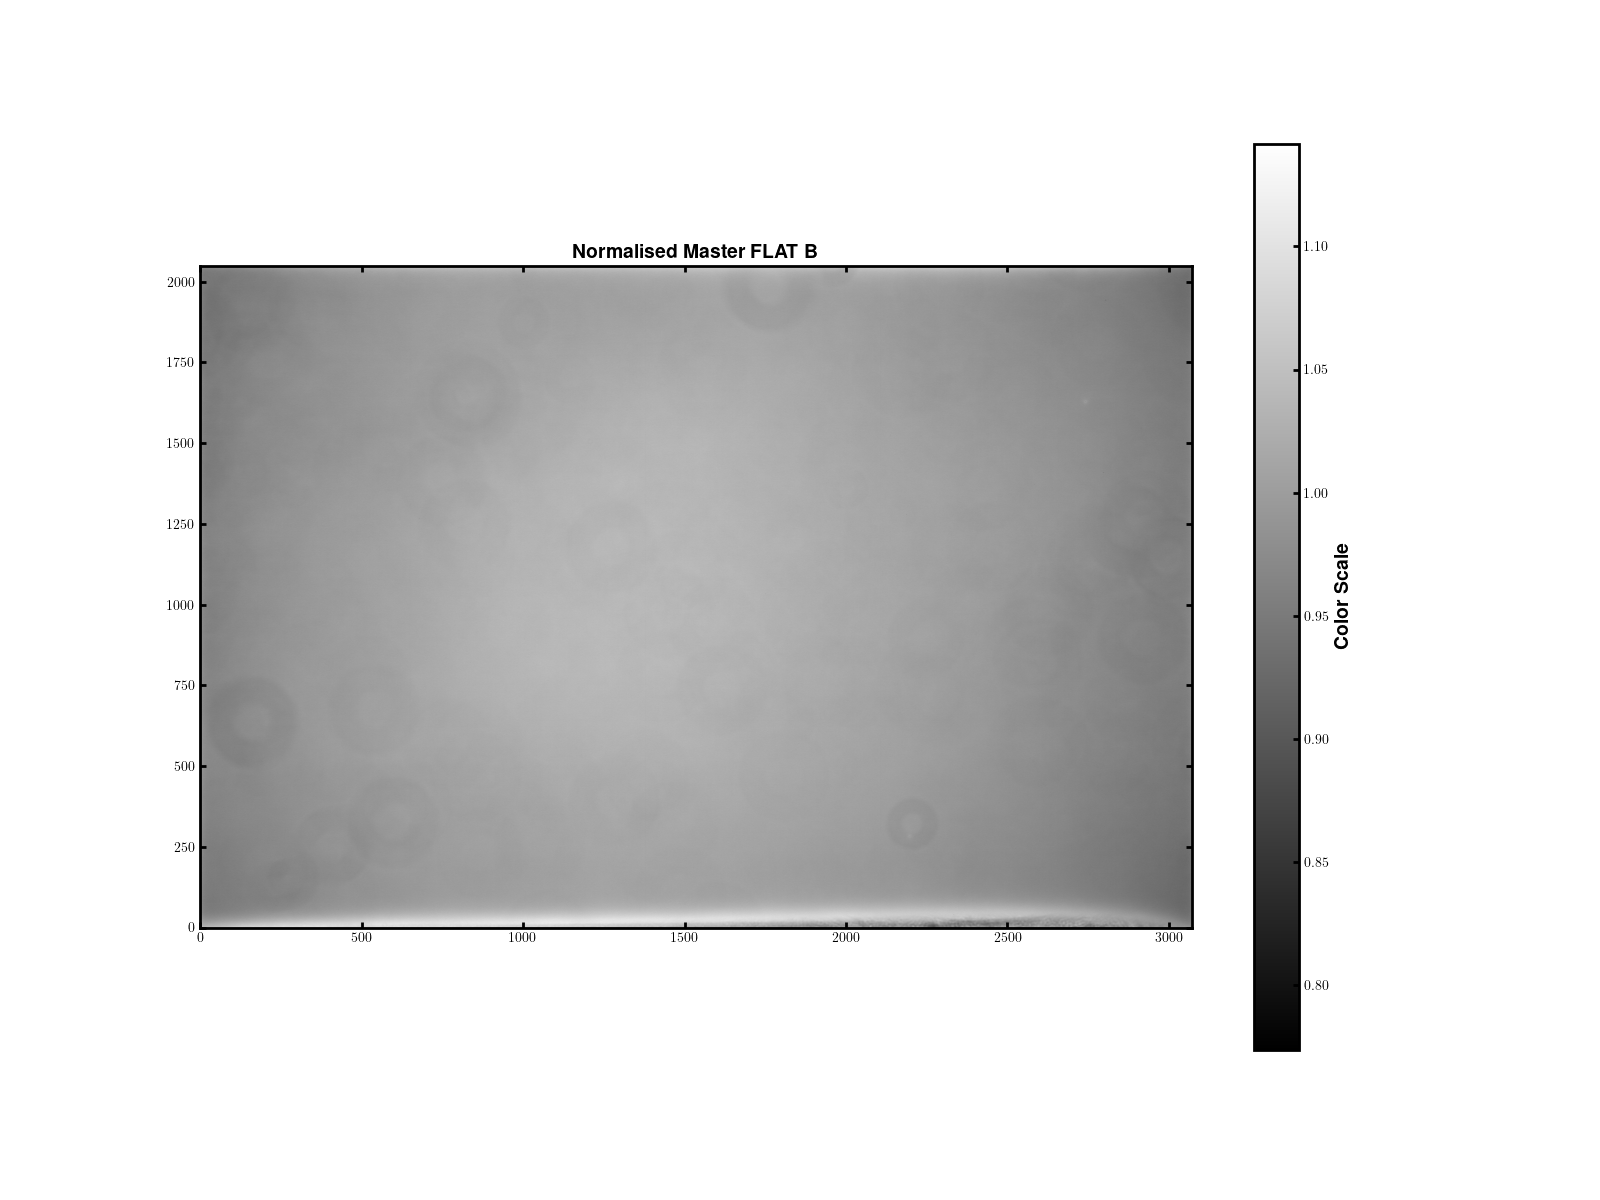
\includegraphics[width=\textwidth]{fig/Normal_Master_FLAT_B.png}
    \caption{Normalized MASTER FLAT frame in the B band}
    \label{normal_master_flat}
\end{figure}

\subsection{Image Registration}
In a further step, we co-add the science frames, but for each band. This is done due to dithering or bad tracking of the telescope since the image might not be perfectly aligned making it complicated to just simply add the data arrays. We use the Python code included in the manual to generate the co-added master reduced science frames for every band by taking the median for every pixel. We set one individual frame from the B-band to be a reference for all other images. An example of a coded reduced master science frame is shown in Figure \ref{co-added}.

\begin{figure}[H]
    \centering
    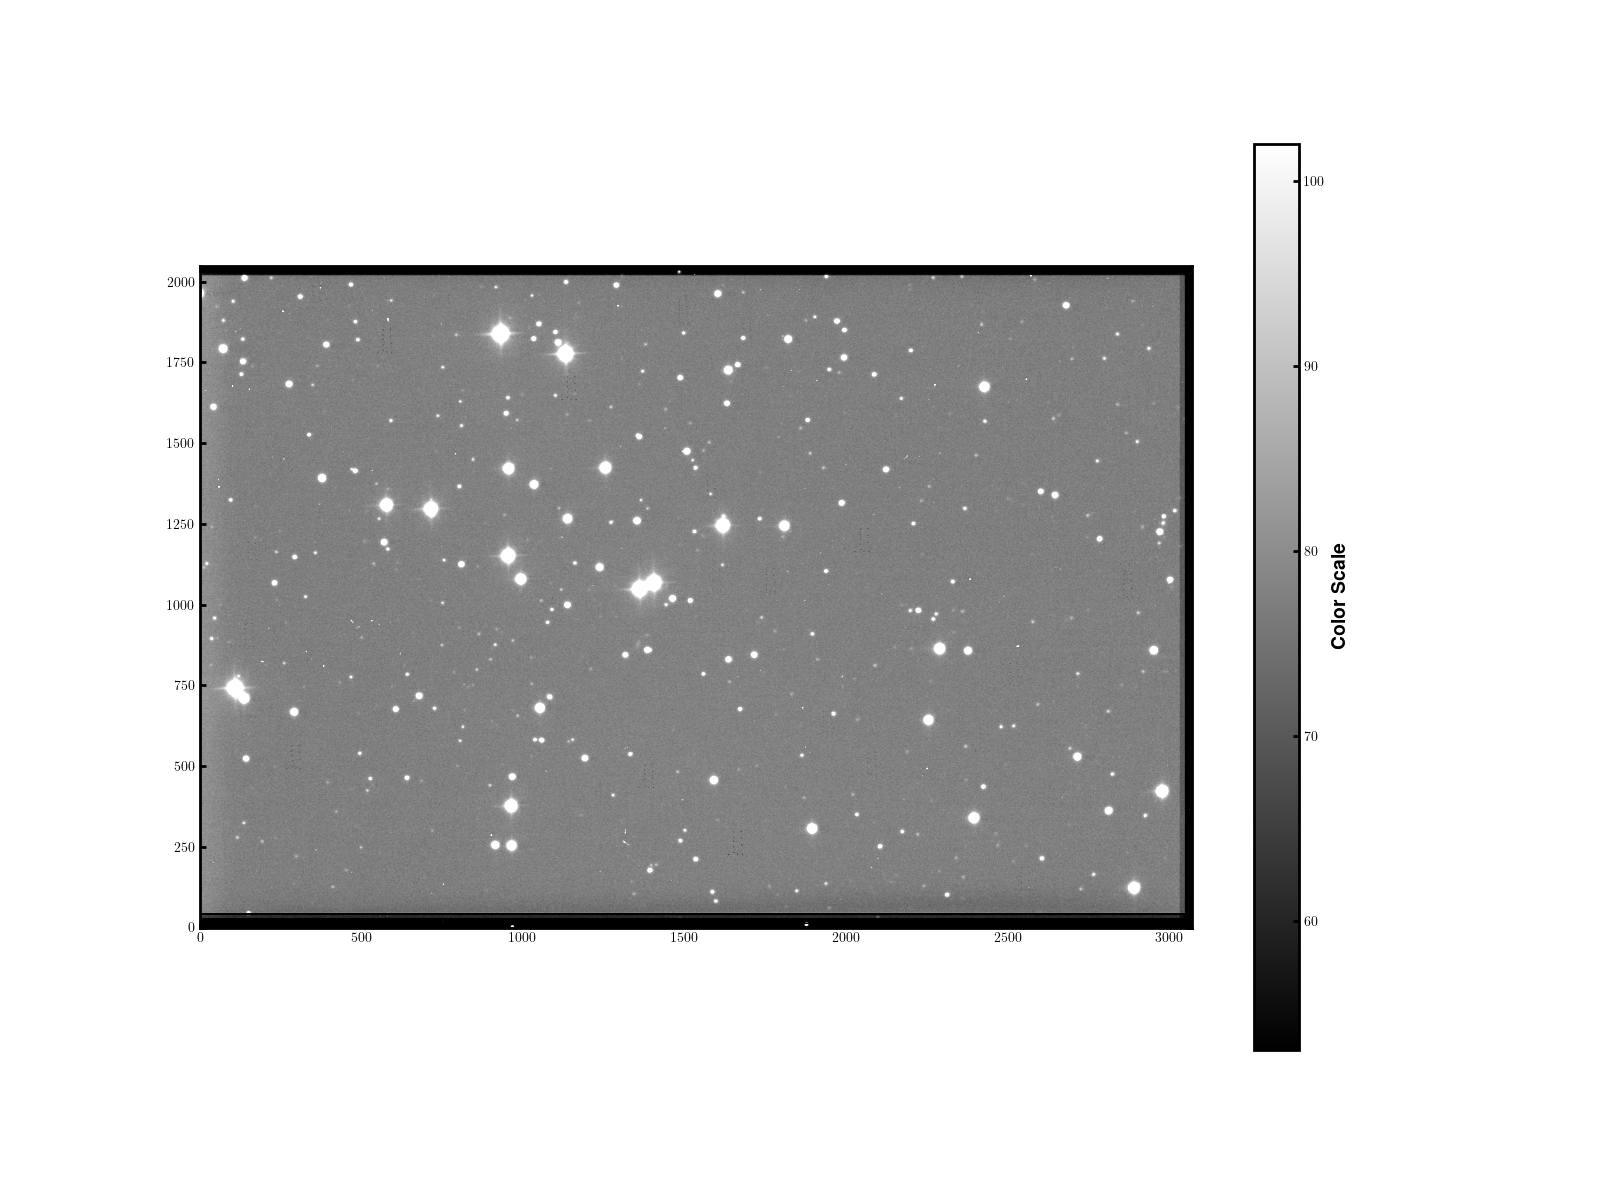
\includegraphics[width=\textwidth]{fig/Co-added_reduced_master_B.png}
    \caption{ Co-added reduced master science frame in the B-band}
    \label{co-added}
\end{figure}

\subsection{Weight Maps}
Each pixel is assigned an individual weight to account for the fact that each pixel has a different sensitivity or signal-to-noise ratio than others. We get a weight map by simply dividing the master flat frame by the maximum value of its flat frame. The resulting weight map, shown in Figure \ref{weighted}, will be later used during the extracting surces from the co-added figurs with source extractor. 
\begin{figure}[H]
    \centering
    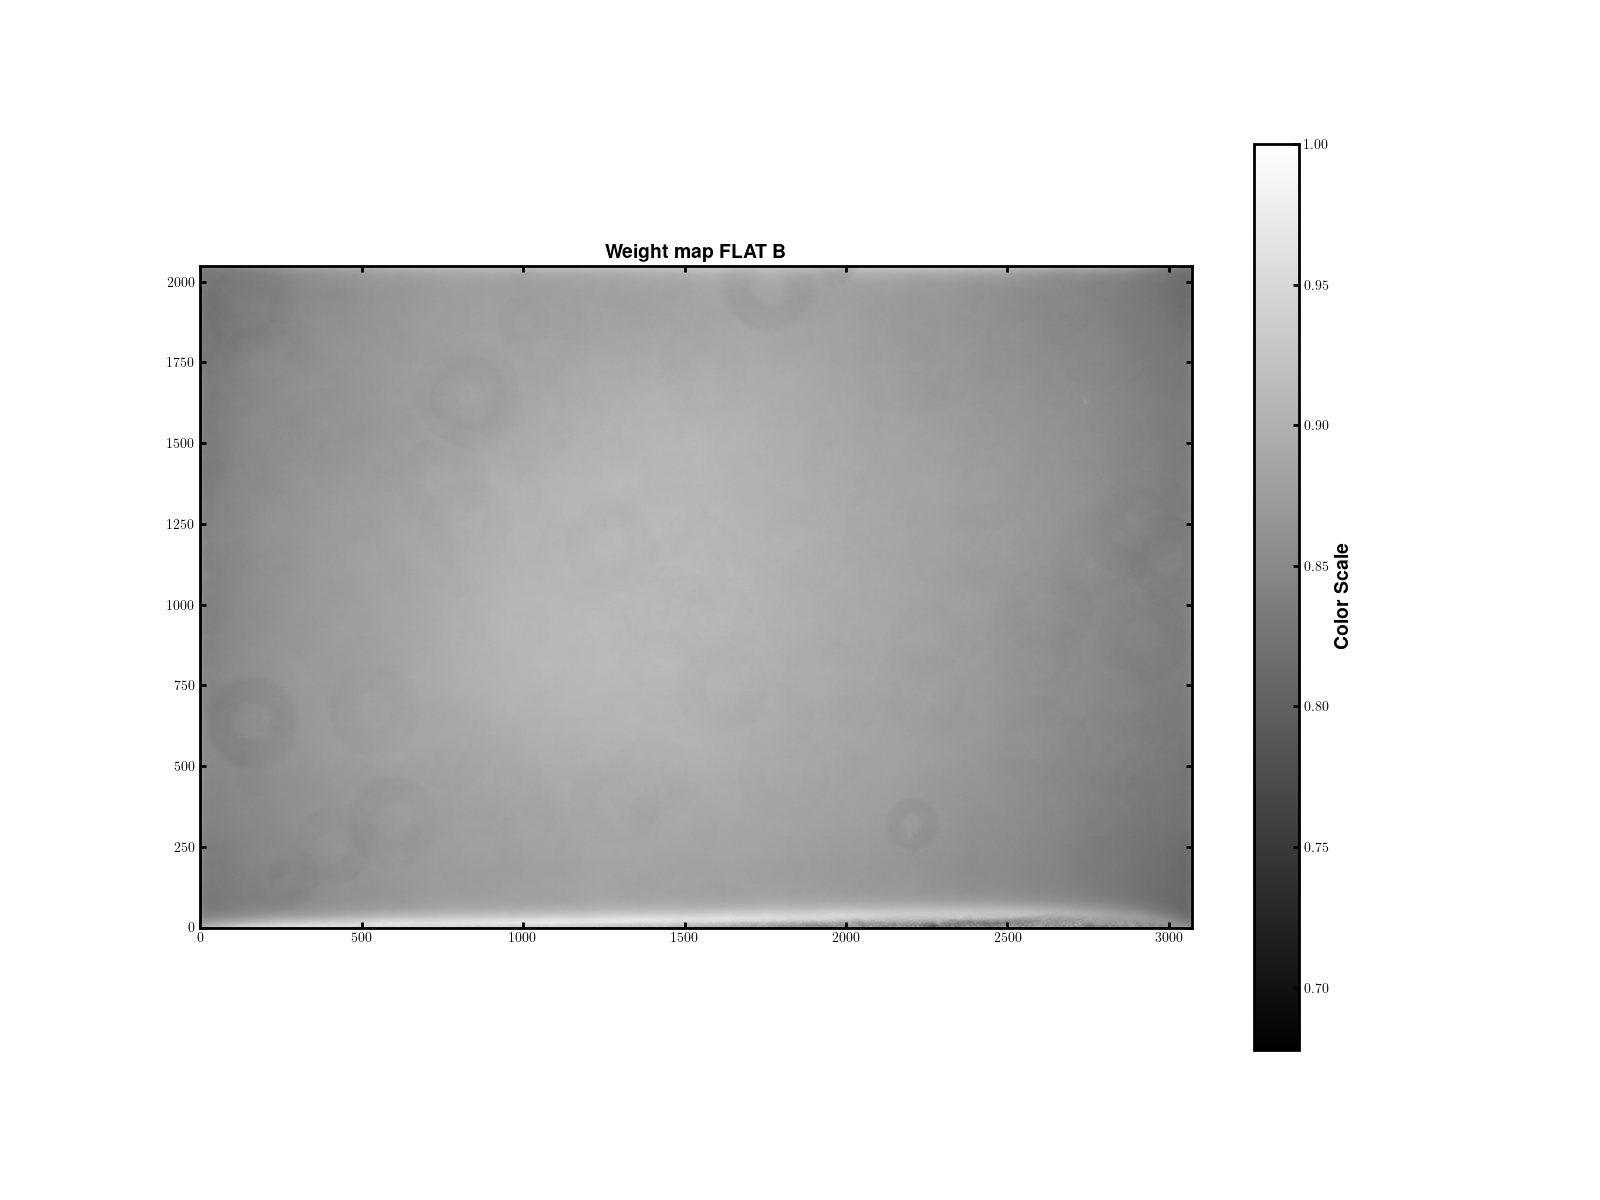
\includegraphics[width=\textwidth]{fig/weightmap_FLAT_B.png}
    \caption{ Weighted master flat frame in the B-band}
    \label{weighted}
\end{figure}

\subsection{Cosmic Ray Subtraction}
Cosmic rays, relativistic charged particles, penetrate the atmosphere and get into the telescope detector. With their high energy, they can saturate pixels and make them dead pixels \cite{lecturenote}. However, we do not need to account for any subtraction for this observation since more than one science frame is present and the master reduced science frame is created. 
\subsection{Background Subtraction}
We subtract the background using photutils library in the following order of steps: We estimate the background, subtract it from the science frame and checking the resulting image using DS9 software. the code provided in the manual is used with the following parameters: nsigma =2, npixels = 5, dilate size = 11, and sigma = 4. We check the subtraction of the background by plotting the histogram of the background region, shown in Figure \ref{background}, as seen, the histograms are centered at zero meaning that the background is successfully subtracted. 

\begin{figure}[H]
    \centering
    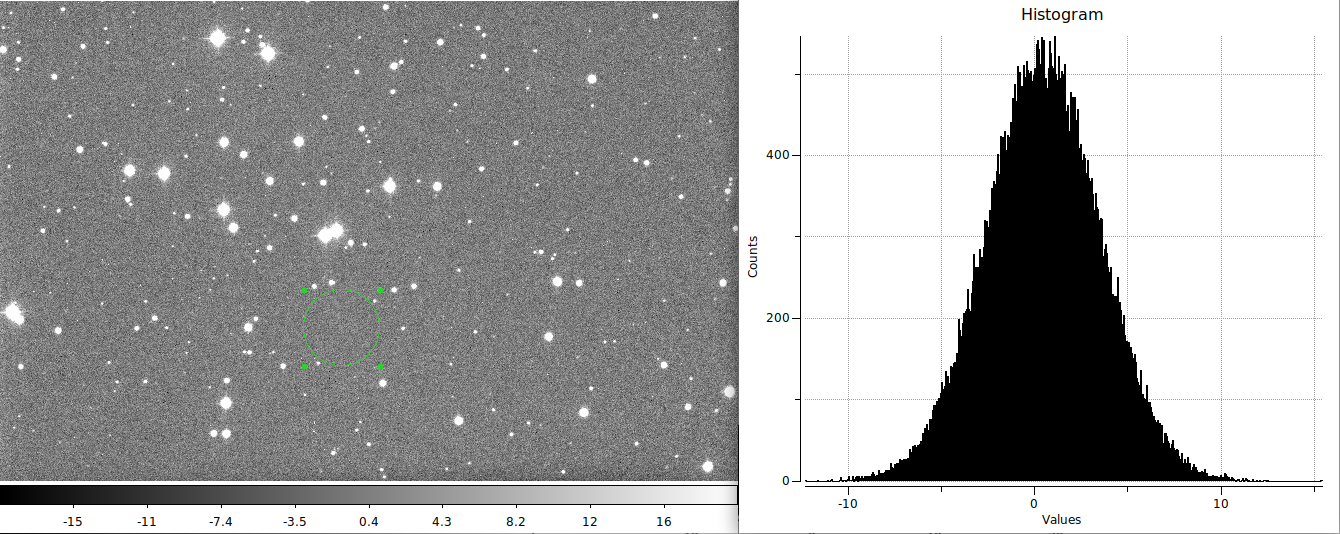
\includegraphics[width=\textwidth]{fig/backsub_B.png}
    \caption{Left: Background subtracted reduced master science frame in the B band. Right: Histogram of background region}
    \label{background}
\end{figure}


\section{Calibration}
\subsection{Astrometric Calibration}
The obtained image is a projection of a curved sky. Therefore, to project it onto the sky coordinates we use an online tool \url{http://nova.astrometry.net/upload} to perform astrometric calibration. This website uses a known catalog of coordinates of stars, so it searches for the objects in the image and gives the coordinates as a result. An astrometric Background-Subtracted Image in the B band is shown in Figure \ref{astrometry}. 

\begin{figure}[H]
    \centering
    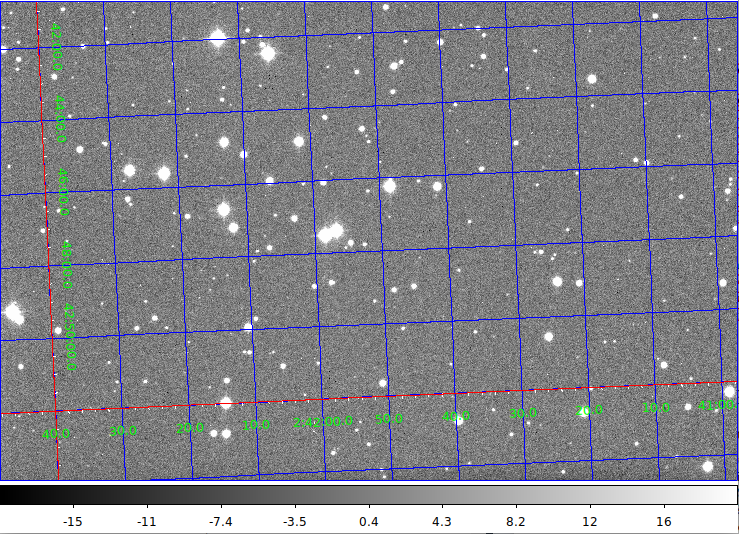
\includegraphics[width=\textwidth]{fig/Astrometric_Calibration_B.png}
    \caption{An astrometric Background-Subtracted Image in the B band}
    \label{astrometry}
\end{figure}

\subsection{Photometric Calibration}
Since no standard star was observed, we select a number of 25 stars in our image and take the mean of magnitudes in each filter. a source extractor is run for all bands separately. We use the commands mentioned in the lab manual and set the parameter MAG\textunderscore ZEROPOINT to zero. Two other parameters were used, DETECT\textunderscore MINAREA, used to set the minimum number of pixels needed to recognize an area, and DETECT\textunderscore THRESH, used to set the sigma threshold of counts for a pixel to be considered a source pixel. Furthermore, we use four combinations of the latter two parameters :  (10,2.5) (5,5), (10,10), (15,40) and (20,100). Finally, a python script was written to combine and detect all stars in three different bands. Figure \ref{parameters} shows three of the CMD plots.

\begin{figure}[H]
    \centering
    \begin{subfigure}{.48\textwidth}
        \centering
        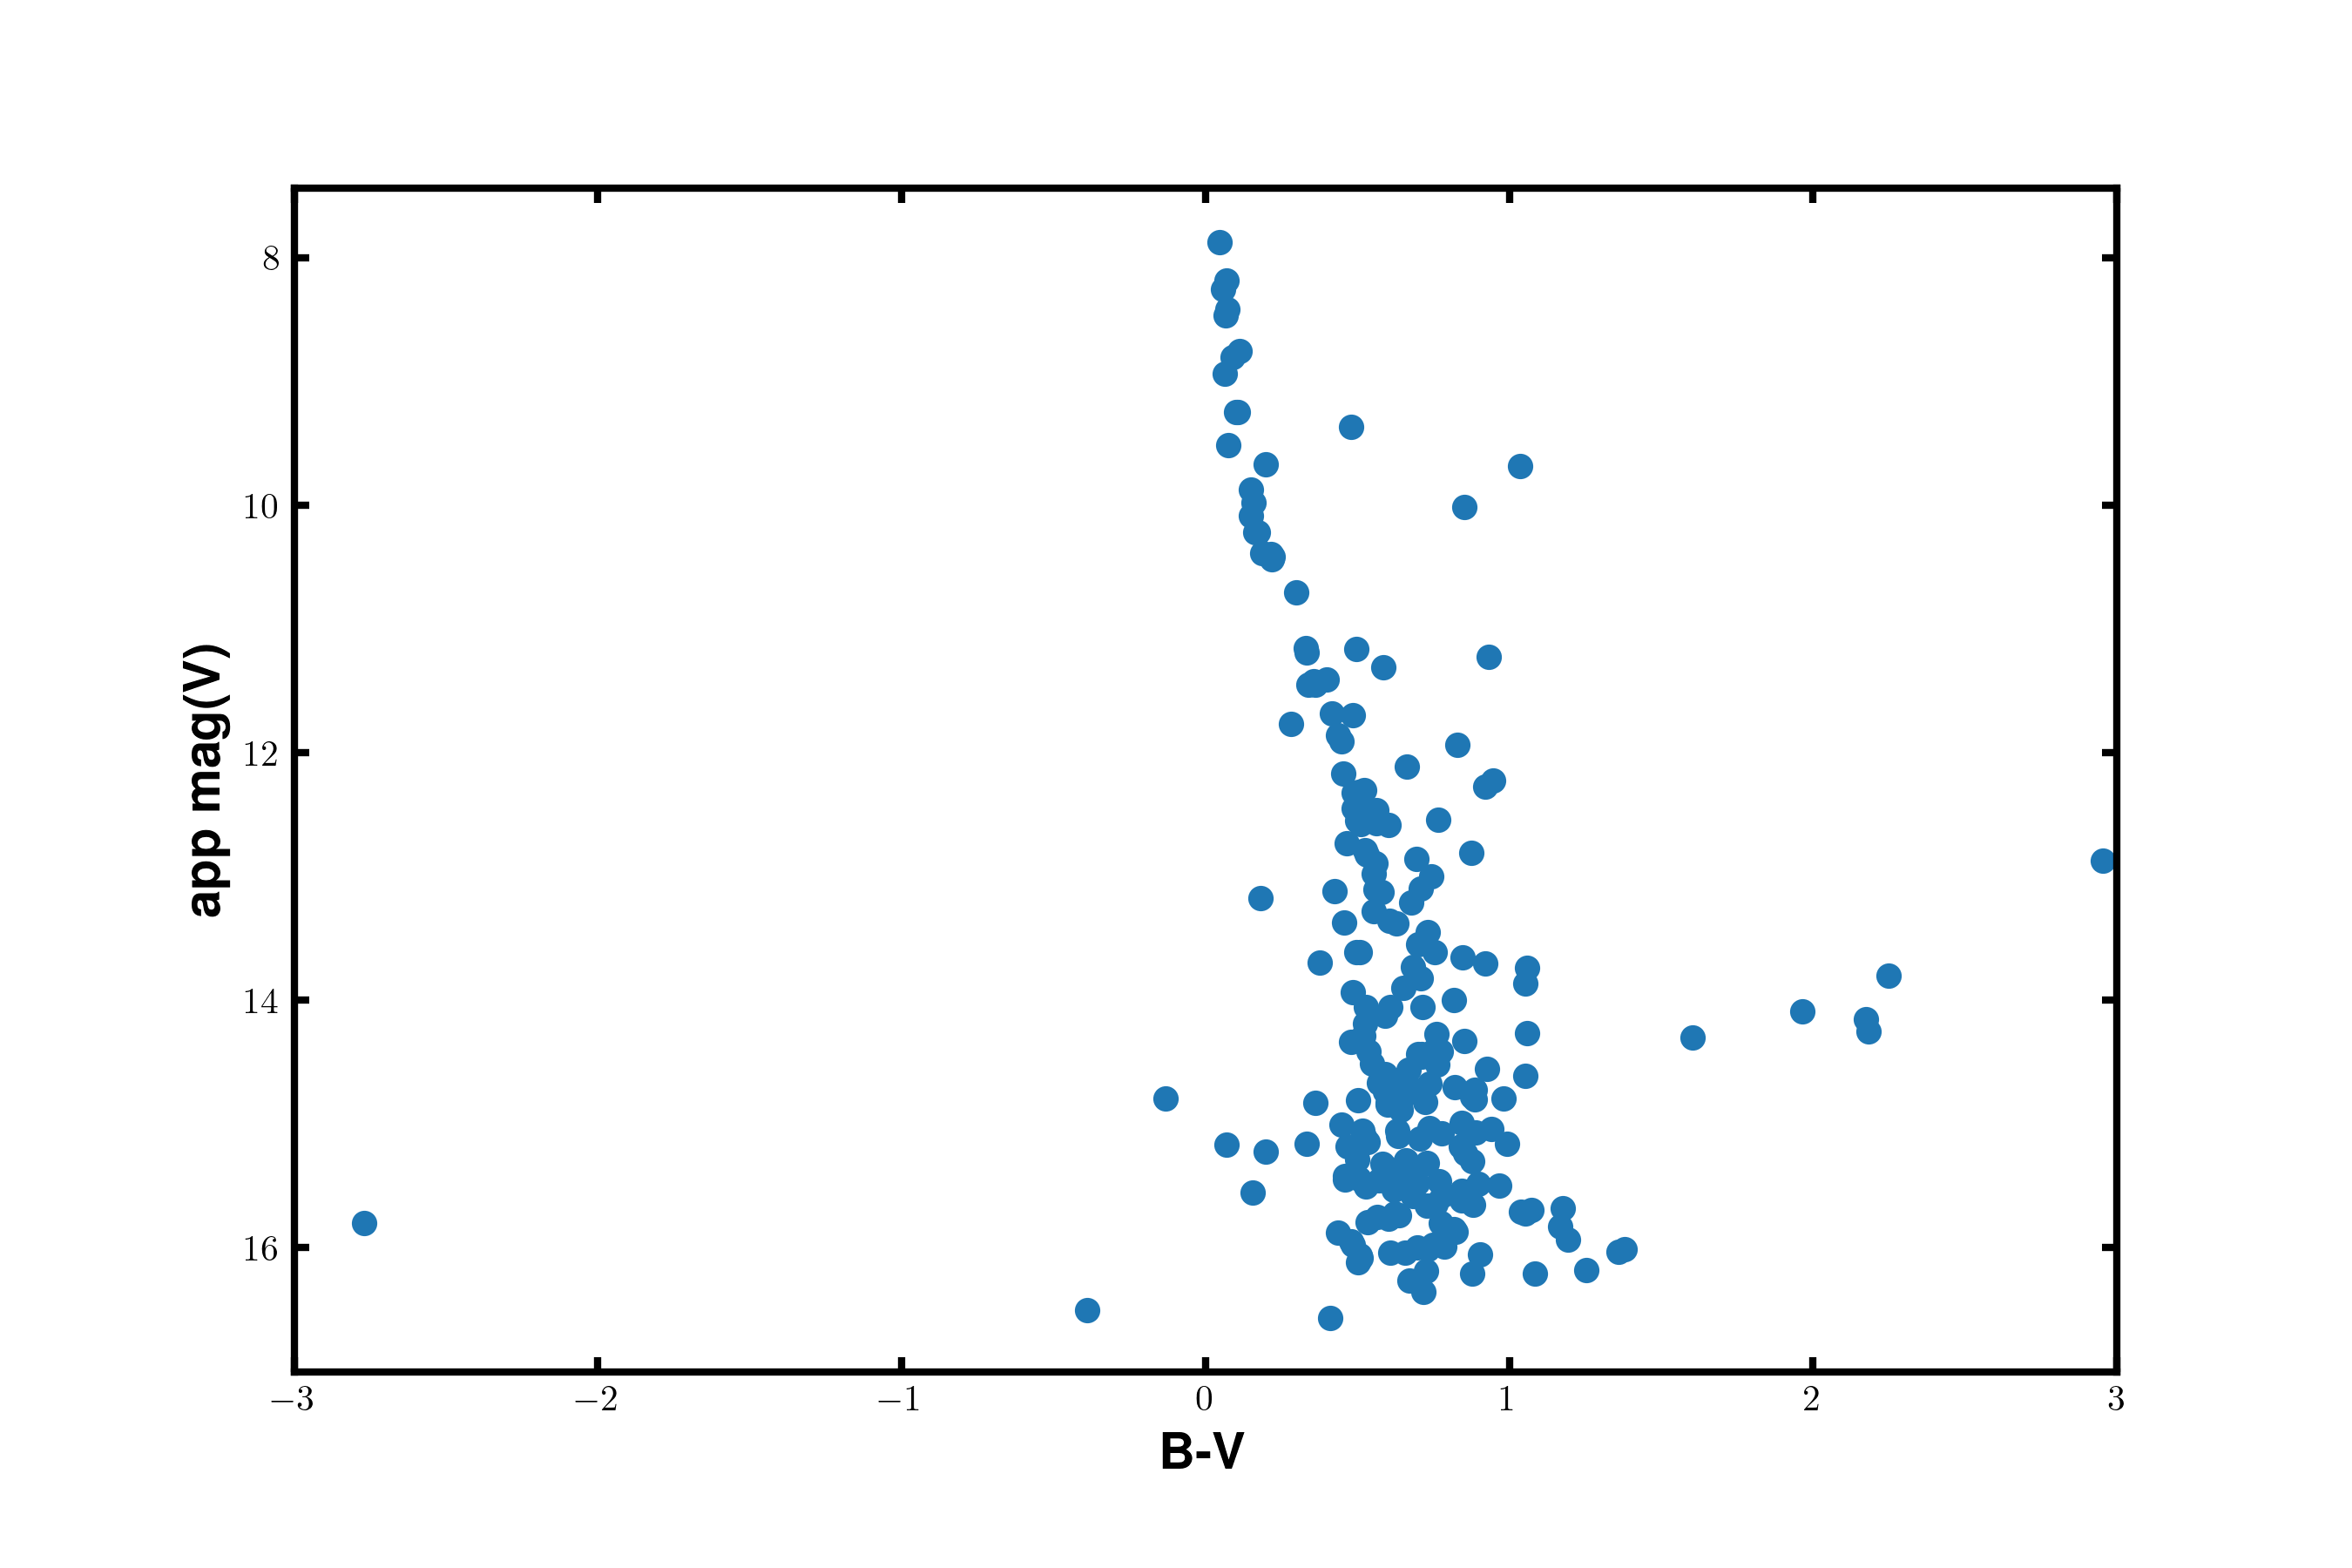
\includegraphics[width=\linewidth]{fig/(5,5)CMD.png}
        \caption{(5,5)}
    \end{subfigure}
    \hfill
    \begin{subfigure}{.48\textwidth}
        \centering
        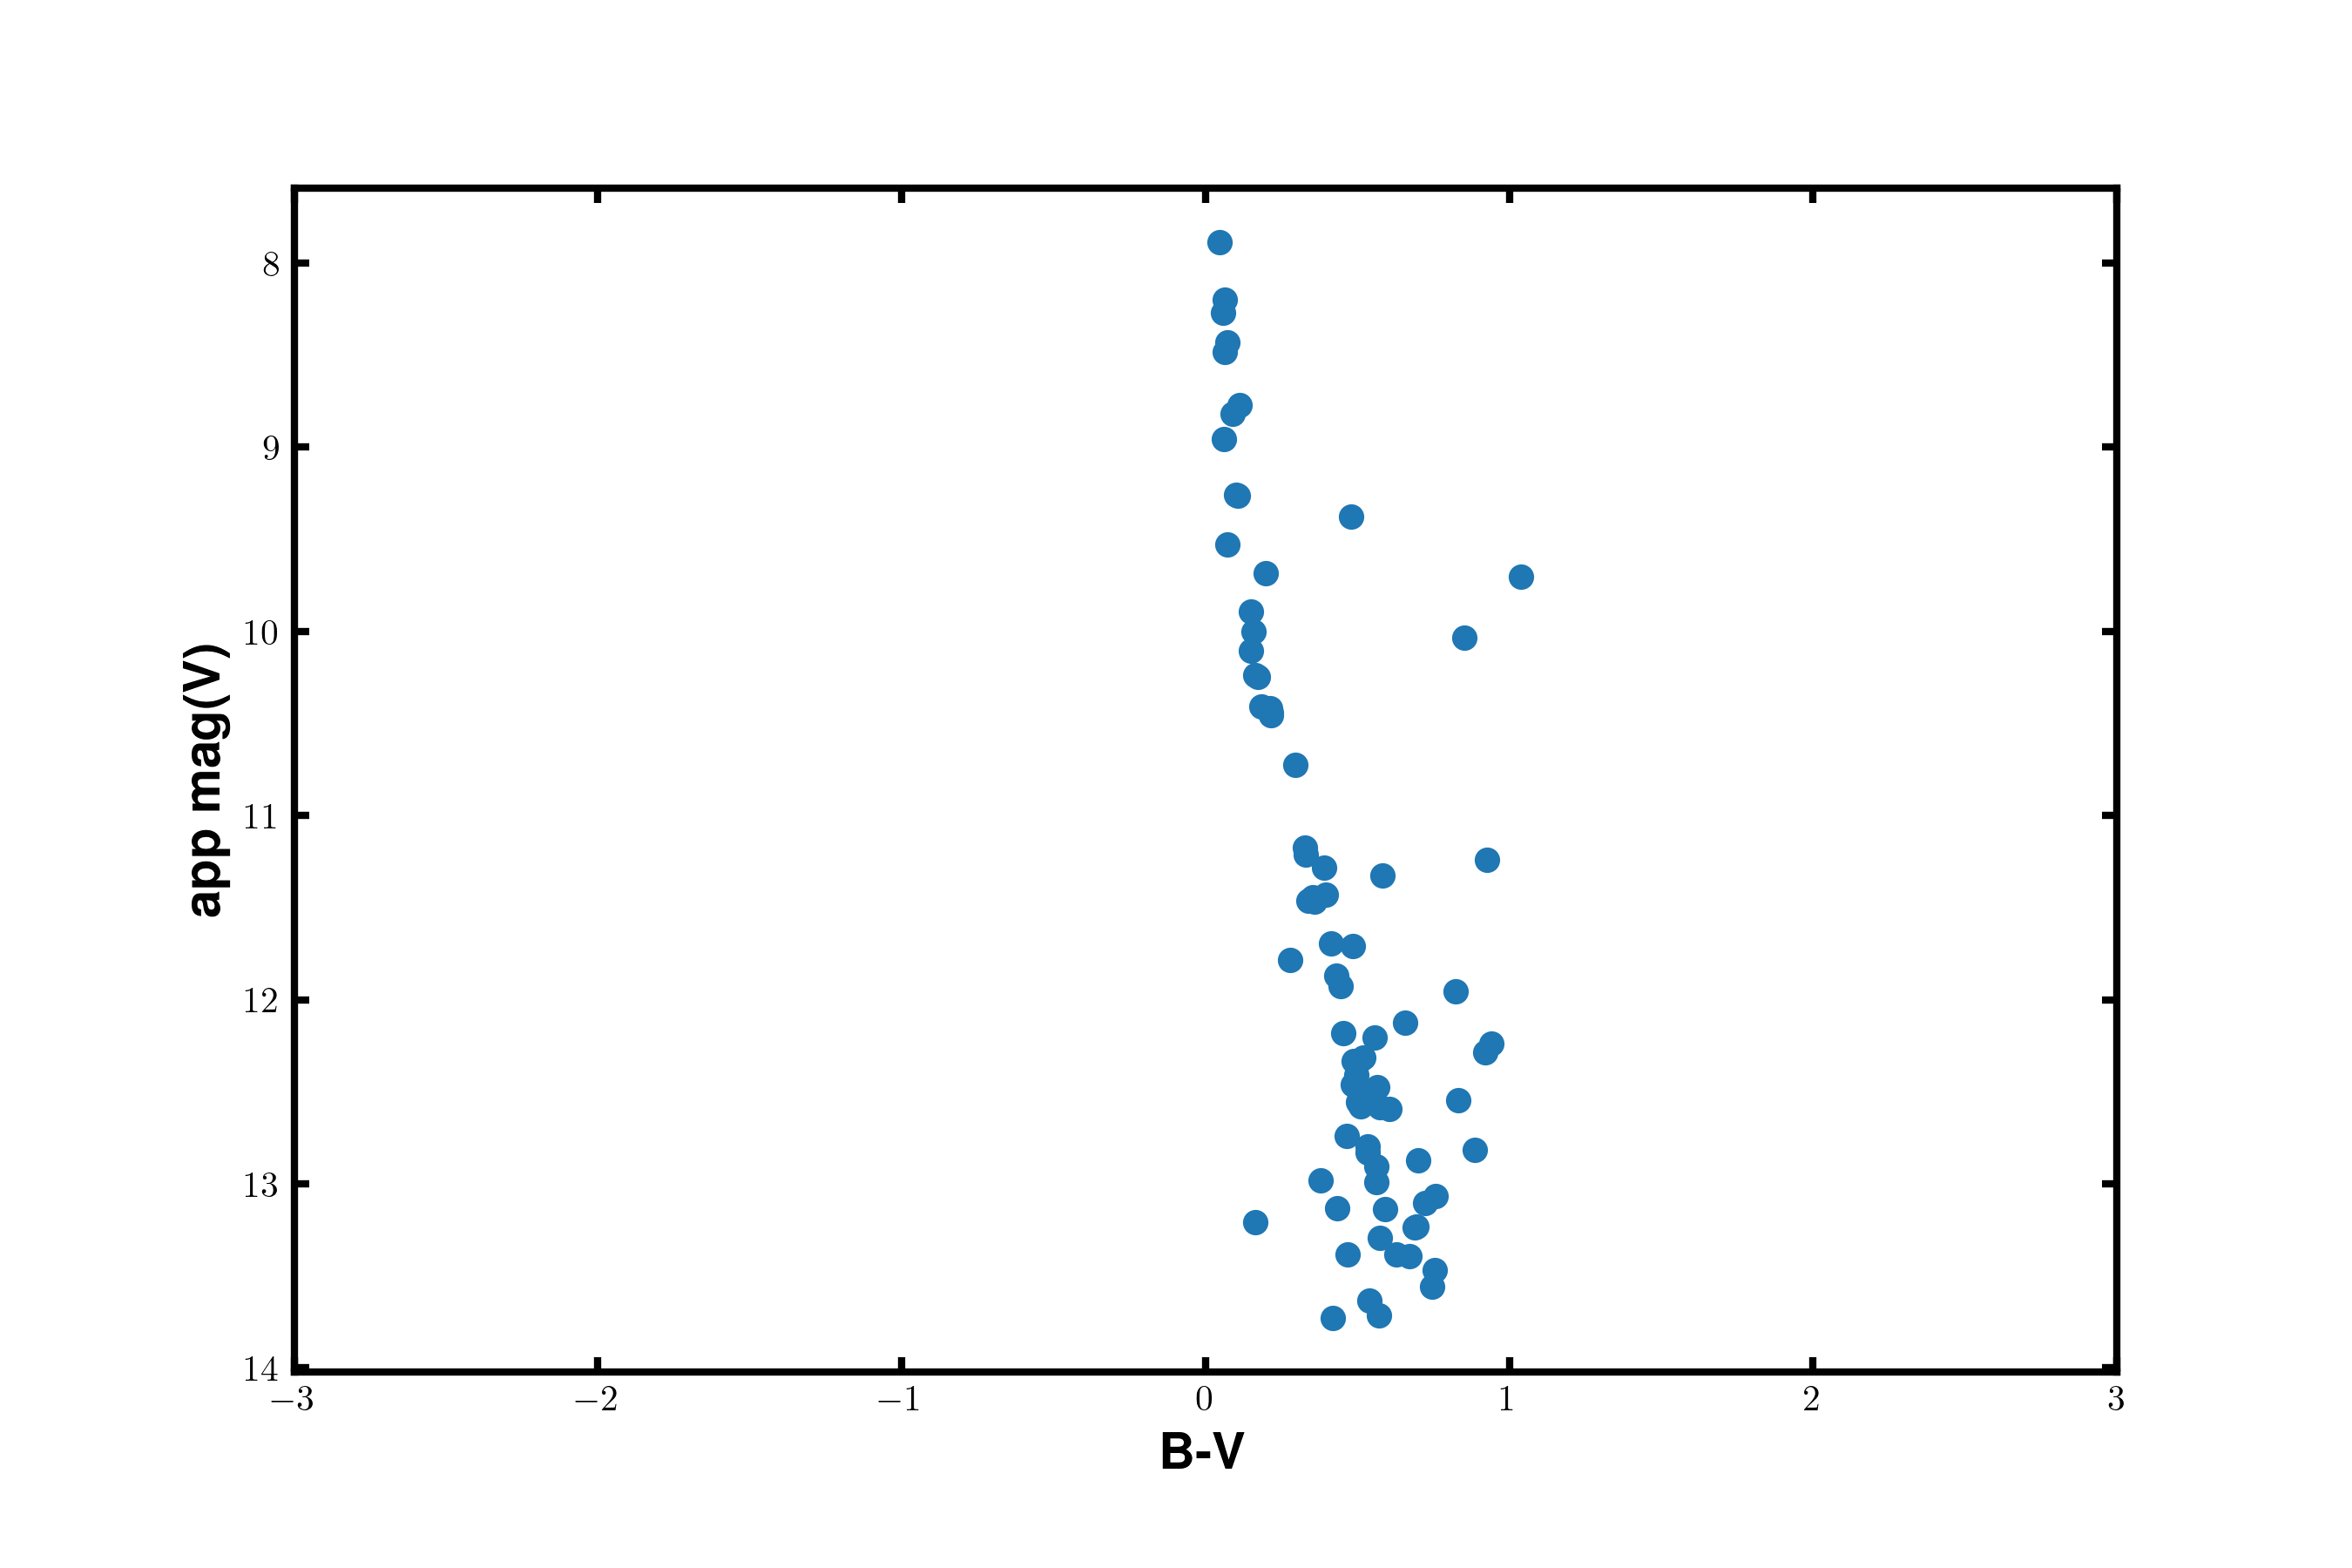
\includegraphics[width=\linewidth]{fig/(15,40)CMD.png}
        \caption{(15,40)}
    \end{subfigure}
    \vspace{0.5cm} % Adjust vertical spacing between rows
    \begin{subfigure}{.8\textwidth}
        \centering
        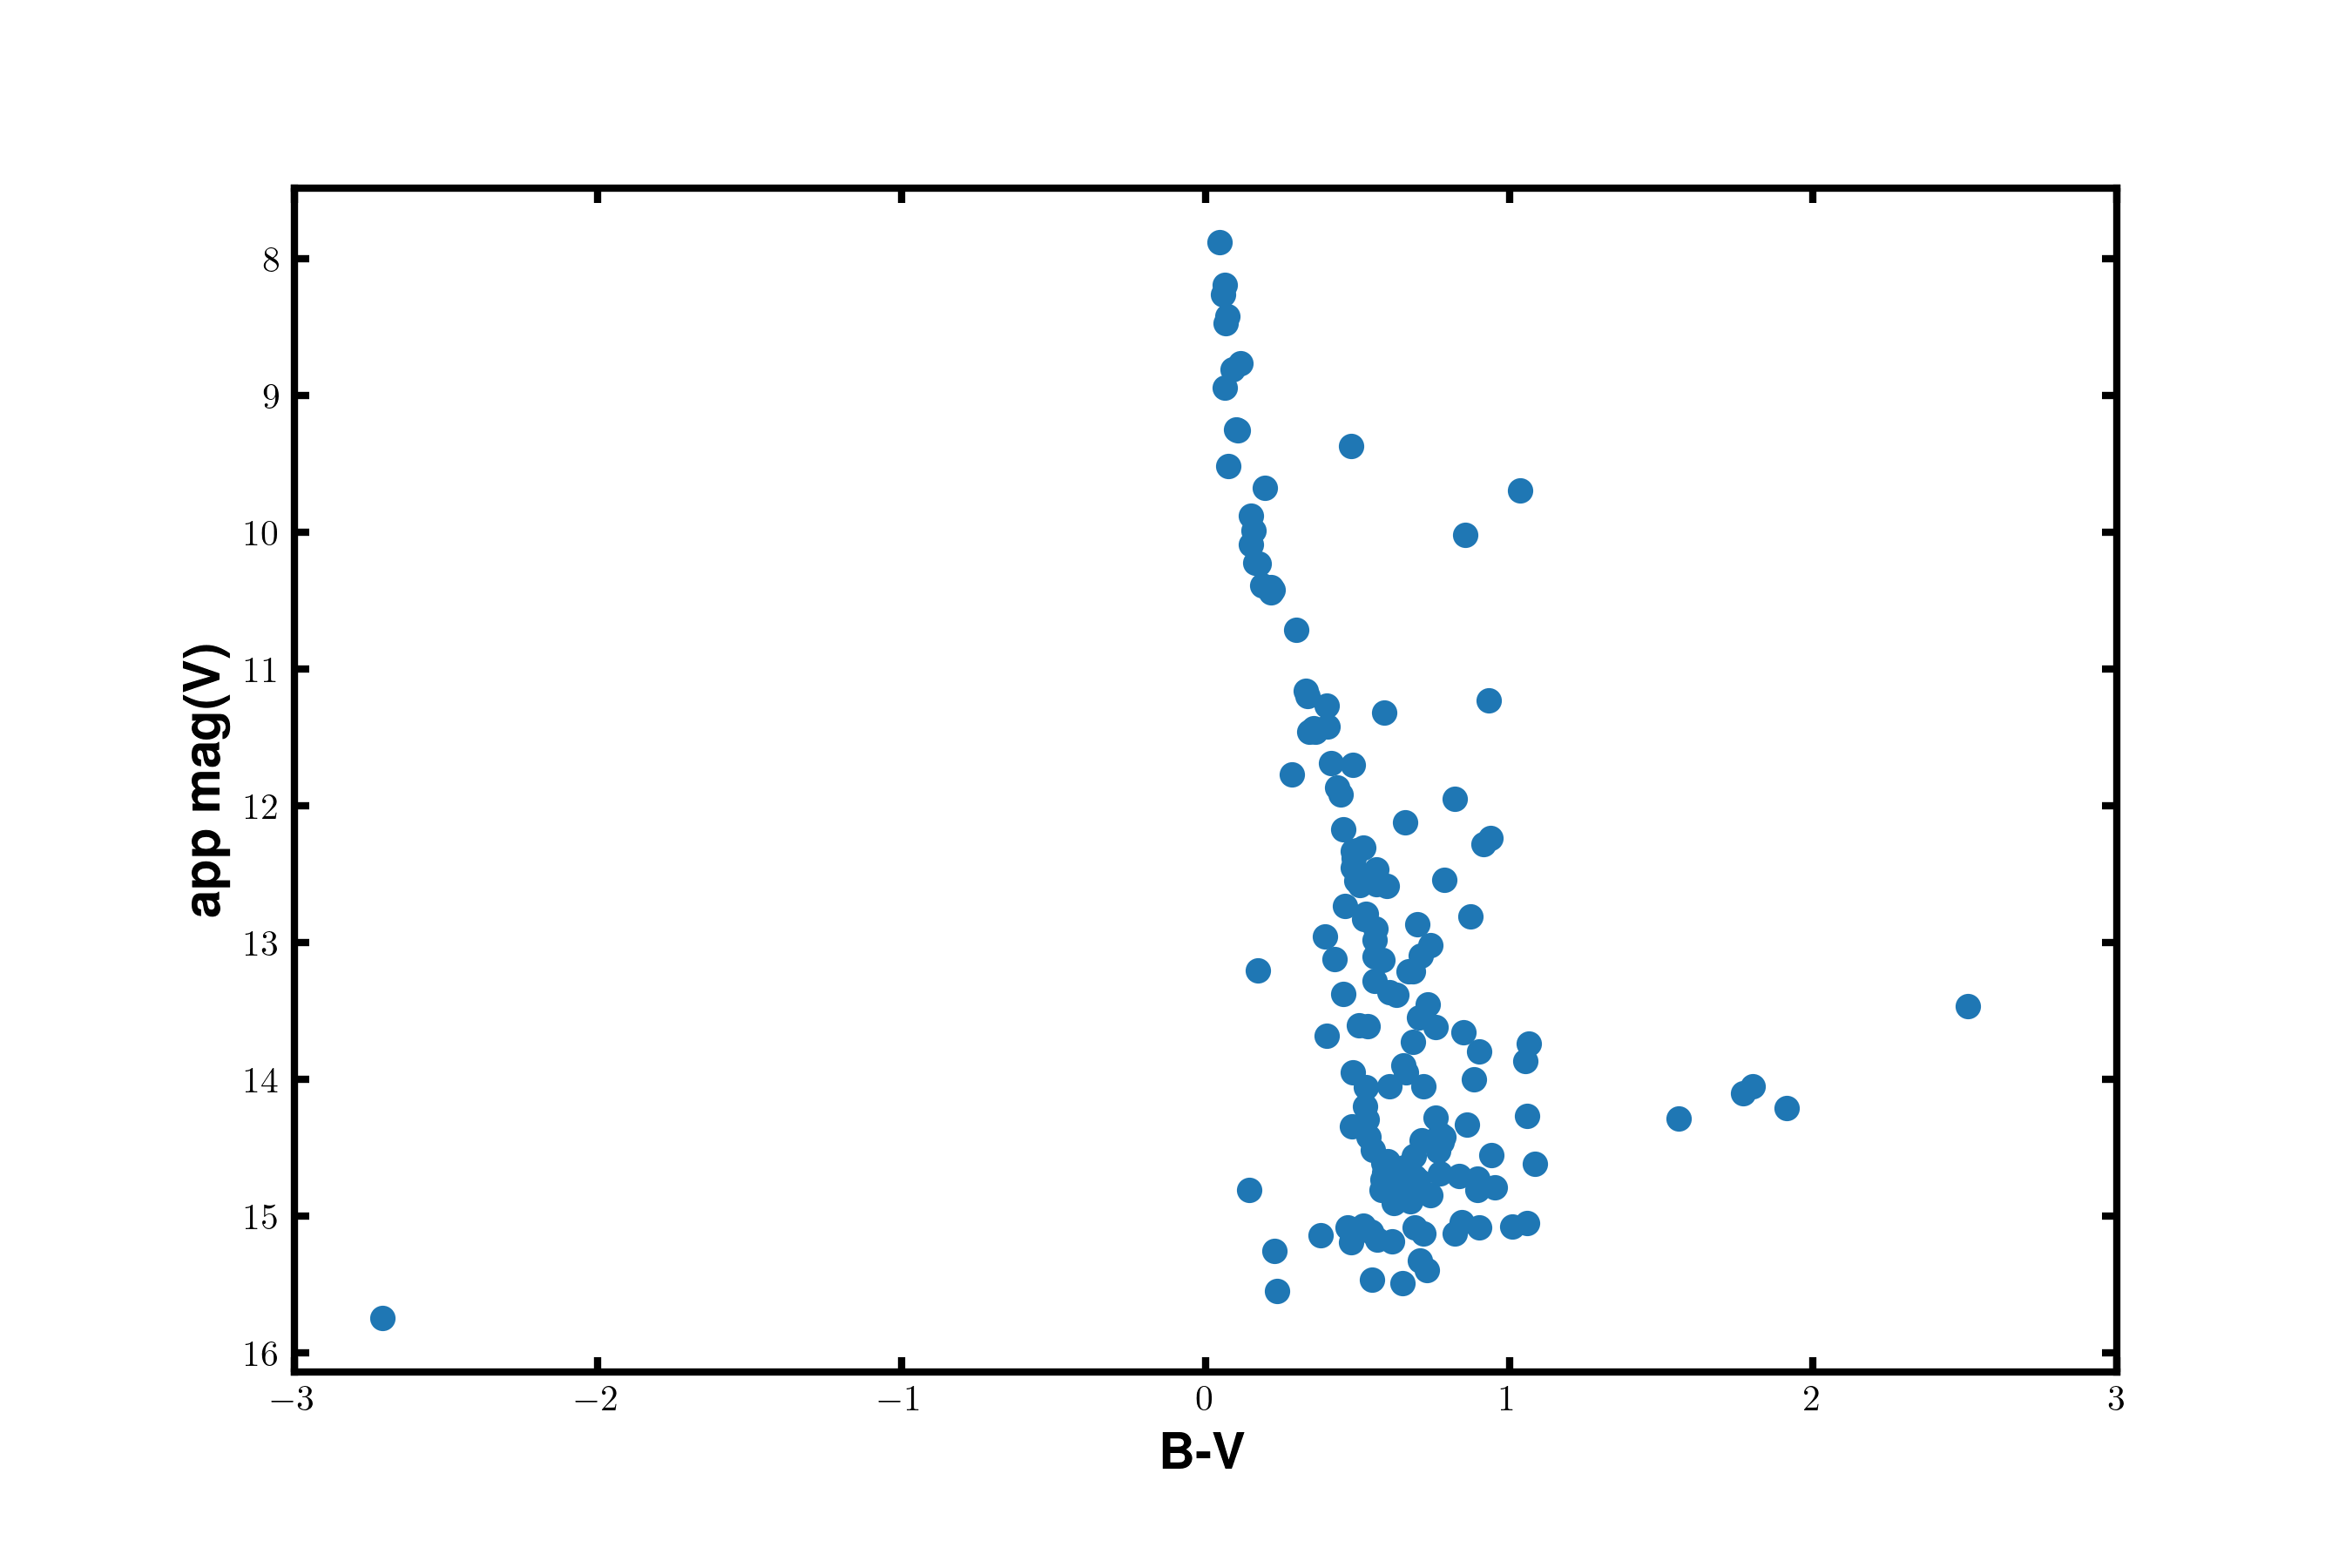
\includegraphics[width=\linewidth]{fig/(10,10)CMD.png}
        \caption{(10,10)}
    \end{subfigure}
    \caption{CMD plots for different used parameters}
    \label{parameters}
\end{figure}

These parameters are based on the number of stars cataloged which is estimated based on the ratio of the solid angle of the star cluster to the one of our telescope. The telescope used has a field of view FOW = 21' $\cdot$ 14' \cite{telescope}, a solid angle of $\Omega_{telescope} = 1.92 \times 10^{-5}$ sr while the solid angle of the cluster is $\Omega_{cluster} = 8.14 \times 10^{-5}$ sr. Meaning that roughly only one quarter of the number of stars is detected. Jones et al \cite{jones}. found 630 stars to be members of the observed cluster, thus, the combination (10,10) is used resulting in 160 detections. 

To get the calibrated CMD, we use the astronomical database SIMBAD \cite{simbad} and correct the apparent magnitudes of the chosen 25 stars in the B and V bands. This is done by adding the difference between the mean value of the magnitude provided by the database and the mean value found by the program for MAG\textunderscore AUTO to the B and V band values of the set of stars chosen. As a result, we get the following correction values: +24.4999 for the B band and +24.6943 for the V band. No errors for these values were given by SIMBAD. The resulting two values are approximate values since only 25 stars were chosen. Therefore, a potential error of the determination of the age and distance of the cluster may arise. 

\subsection{Cropping the Image}
Cropping of a FITS file for the source extractor to choose stars from the clusters and have a proper CMD diagram. However, since the field of view of the used telescope is smaller than the angular extent of the cluster (35' \cite{m34}), there is no need for cropping the image. 

\section{Data Analysis}

\subsection{Extinction}
One has to account for the effect of extinction, star appearing dimmer due to the presence of dust in the interstellar medium \cite{lecturenote}, by correcting it by adding a constant factor to each magnitude. In this analysis, we set the extinction factor E(B-V) to zero as it is smaller than the accuracy achieved in Bonn. 

\subsection{Isochrone Fitting}
In this part of the analysis, isochrones from the Geneva database for different values of metallicities are used: Z = 0.001, 0.004, 0.008, 0.020, 0.040, and 0.1. The ages of these isochrones range from $10^{3}$ to $10^{9}$ years \cite{isochrones}. Furthermore, the best-fitted isochrone will be used to determine the age, metallicity, and distance of the cluster. 

Before fitting, we exclude the isochrones that for low V have shapes that are not compatible with the cluster. A higher metallicity makes stars with masses below 4$M_\odot$ cooler and dimmer resulting in having too many unexplained stars with V mangnitudes less than the end of the isochrone. On the other hand, a too high value of the metallicity makes the isochrone have a tail reaching below the stars with the lowest V magnitudes. An example of unfulfilling the selection criteria is shown in Figure \ref{exclusion}. 


\begin{figure}[H]
    \centering
    \begin{subfigure}{.8\textwidth}
        \centering
        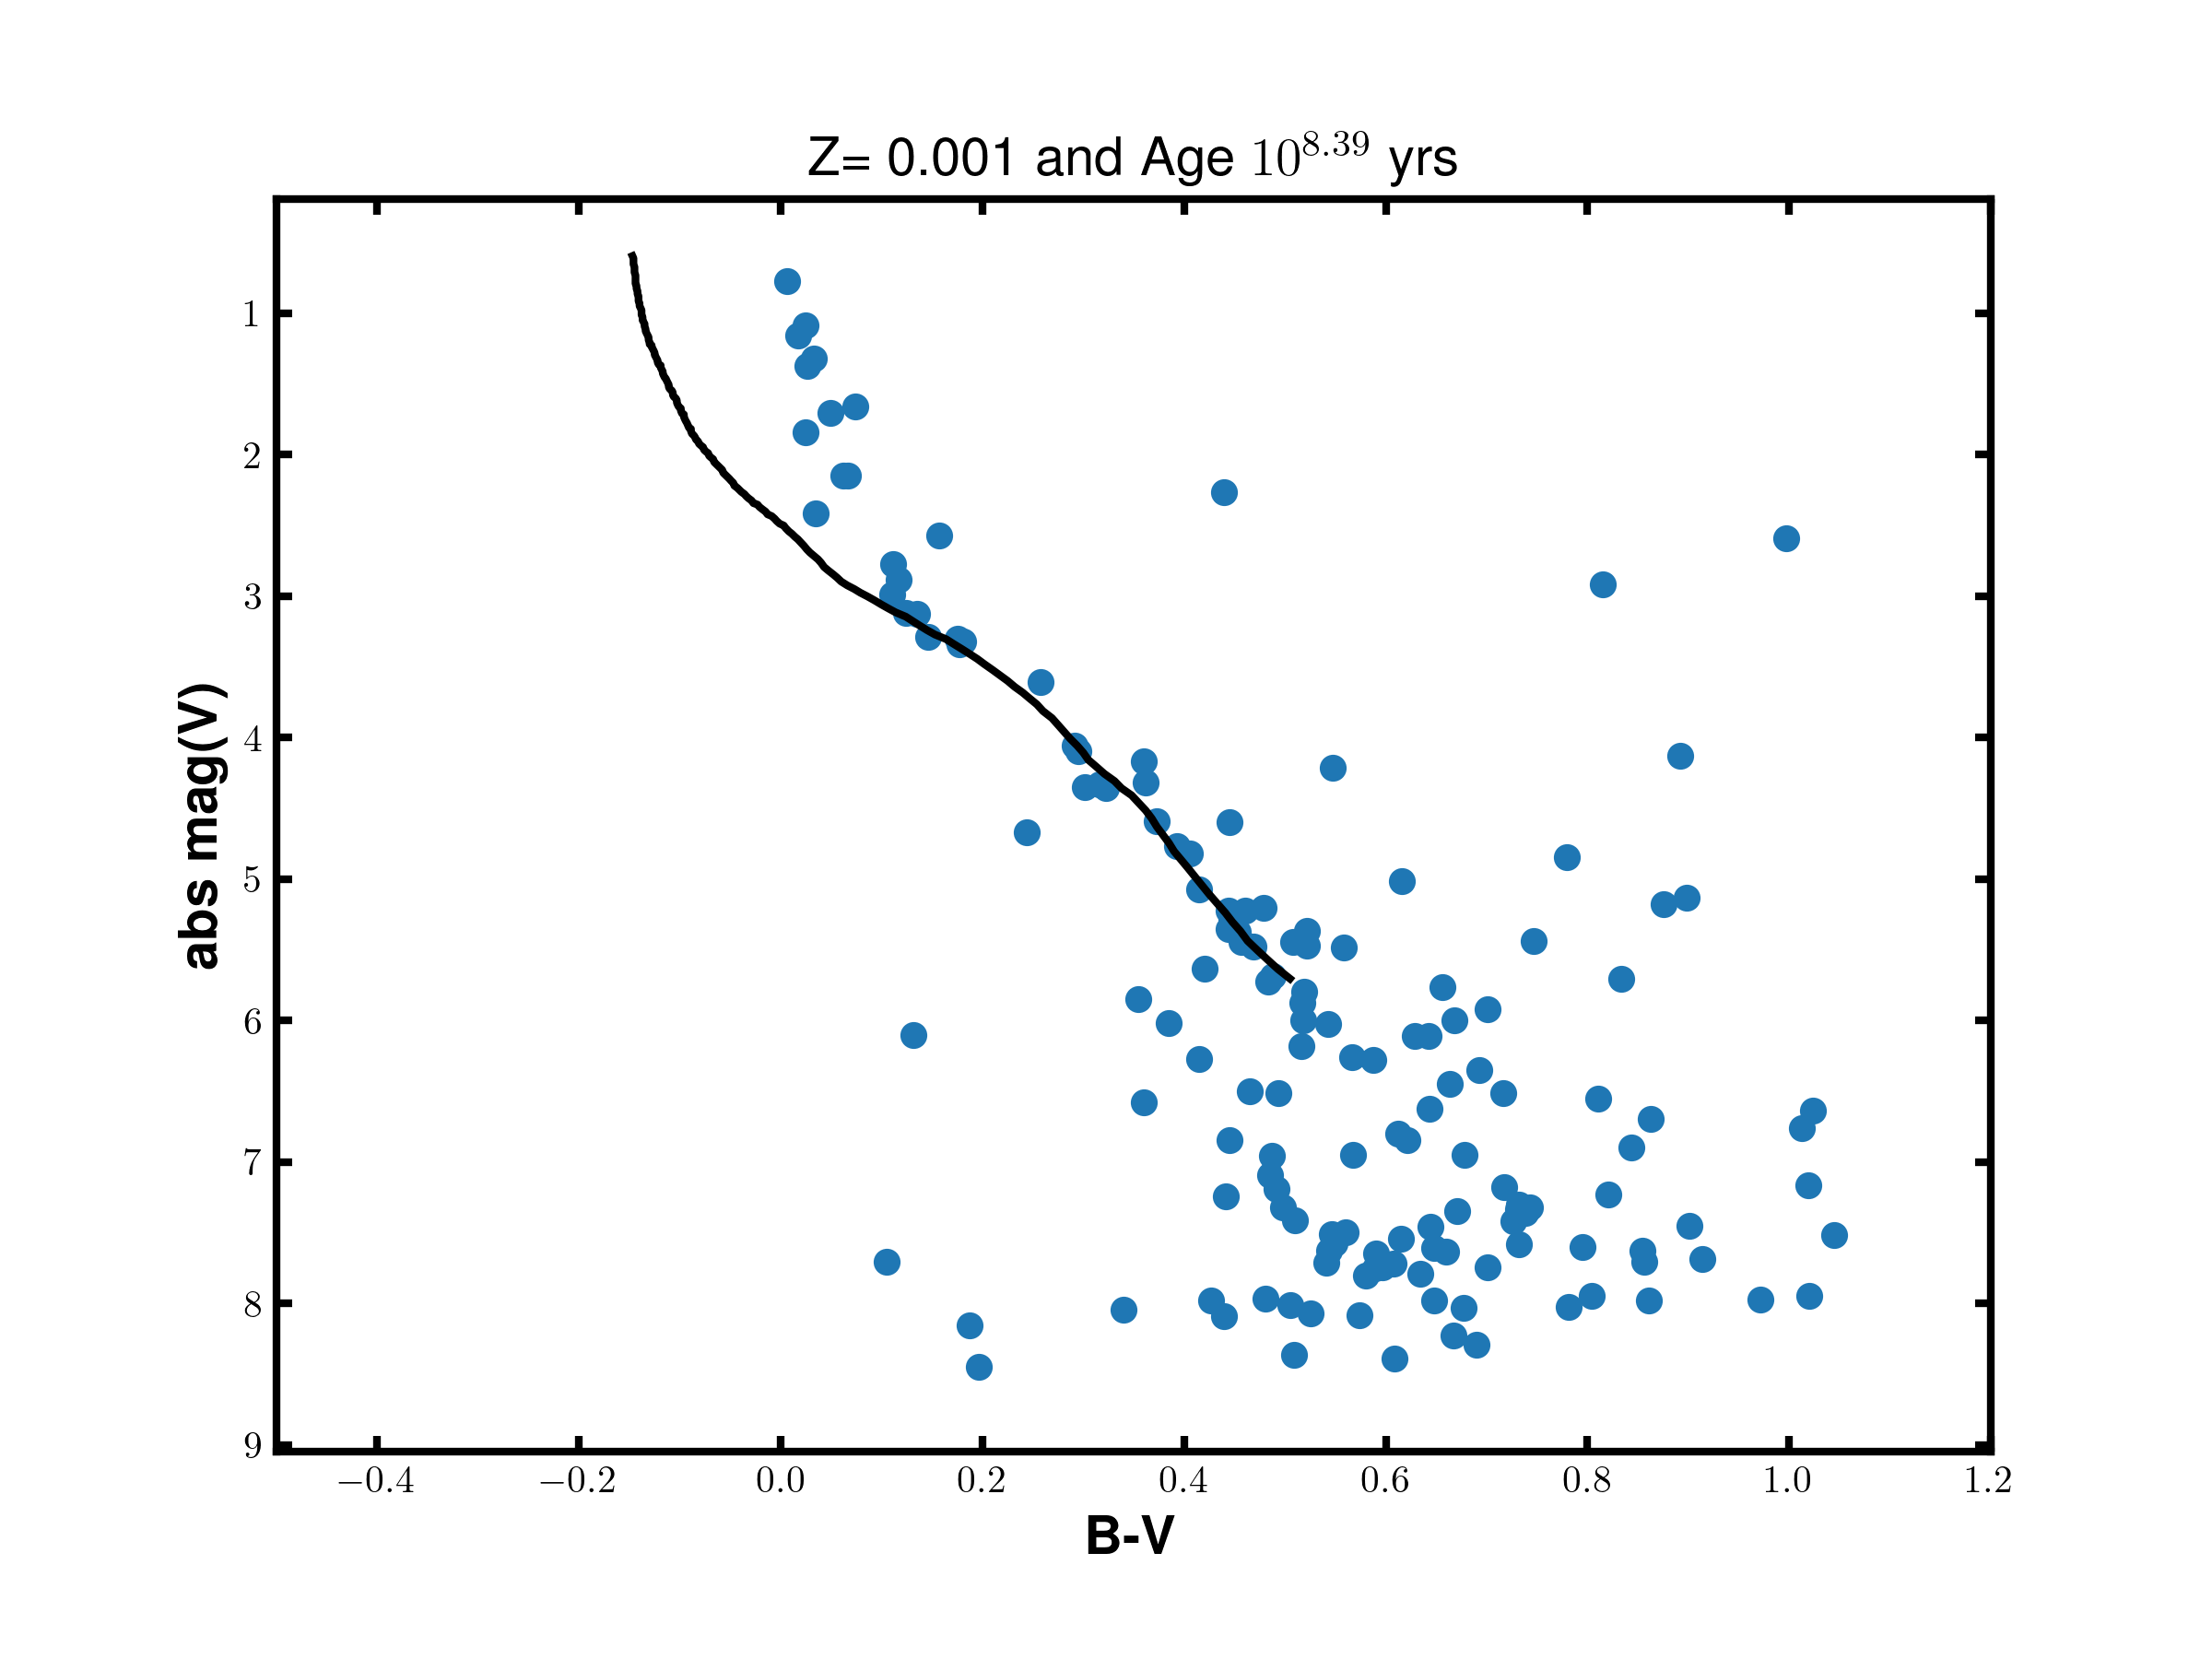
\includegraphics[width=\linewidth]{fig/iso_z001_839.png}
        \caption{}
    \end{subfigure}

    \begin{subfigure}{.8\textwidth}
        \centering
        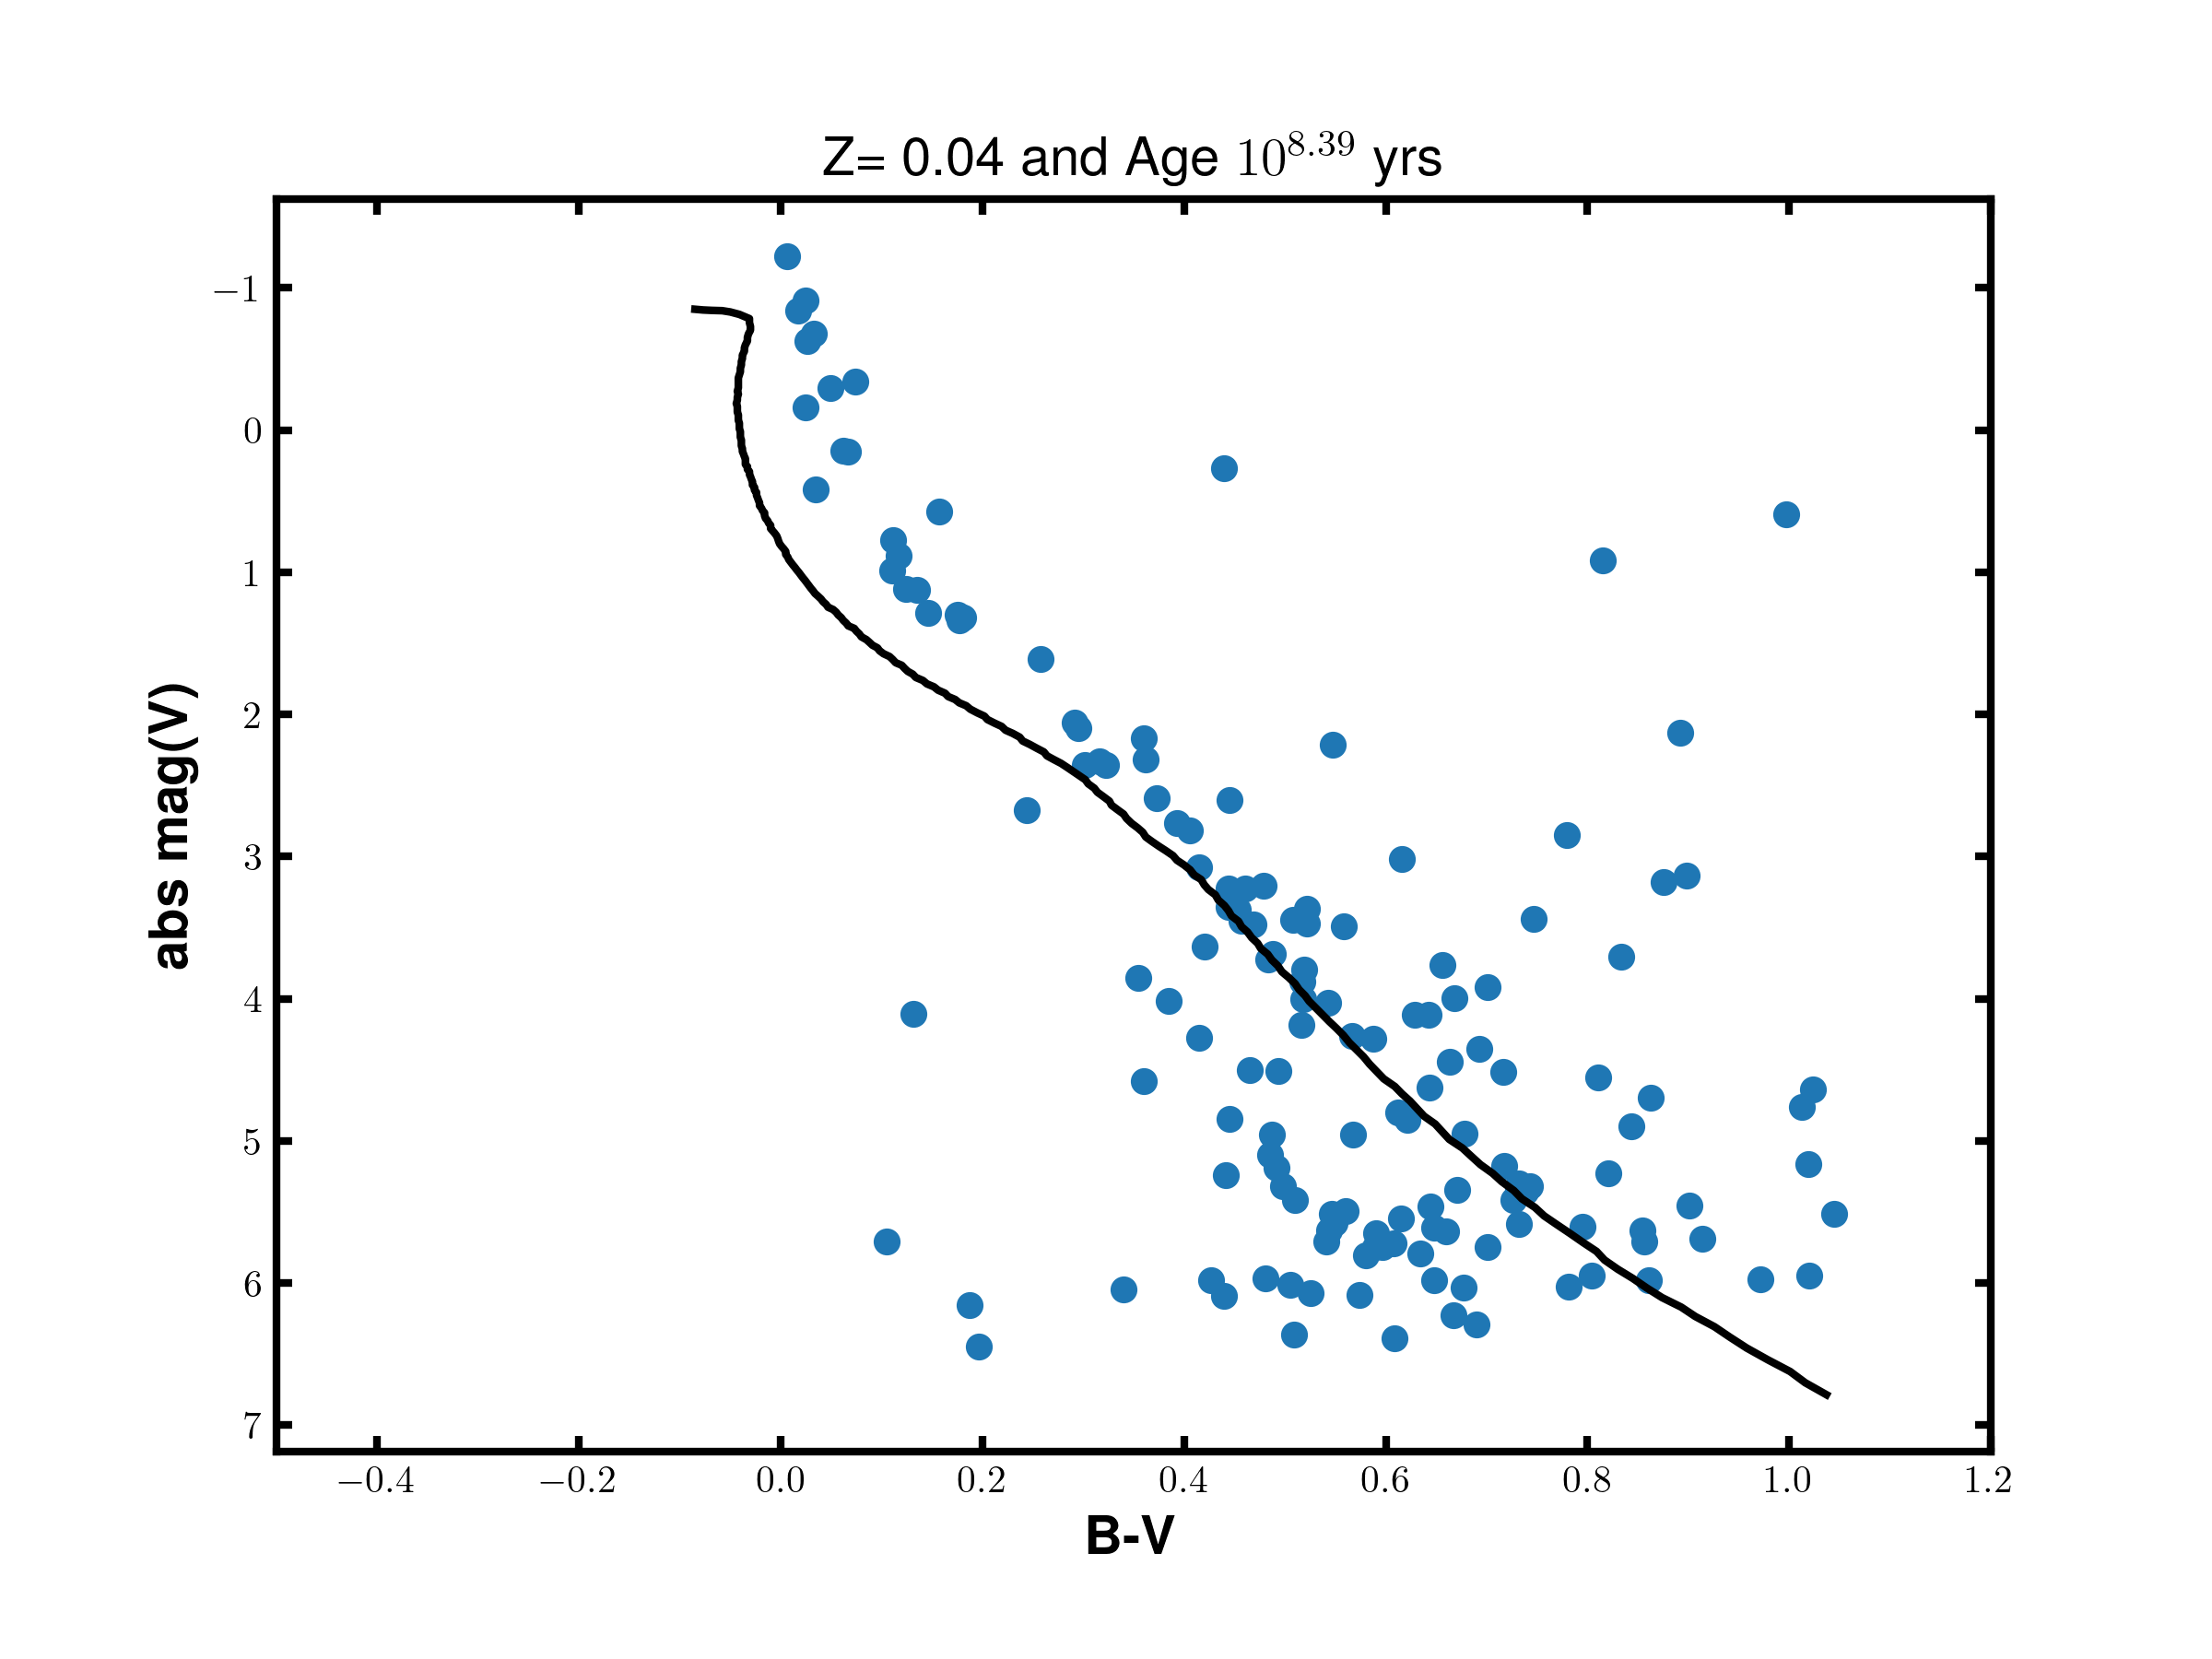
\includegraphics[width=\linewidth]{fig/iso_z040_839.png}
        \caption{}
    \end{subfigure}
    \caption{Top: B-V plot for a too low metallicity. A lot of unexplained stars below the isochrone are present. Bottom: B-V plot for the case of too high metallicity, the isochrone has a tail below the data points}
    \label{exclusion}
\end{figure}

The two methods provided in the manual are not used since the globular cluster is open and there are no stars in the cluster with $B-V < 0$. Instead, we wrote a Python routine \ref{python} to calculate the root mean squared residuals between the data of stars in the CMD and the isochrones. This routine, for all applicable isochrones, goes over different V-shifts and calculates the residuals of the isochrone for every different shift. Following this analysis, the best fit obtained with the lowest residuals corresponds to the isochrone with Z = 0.02 and an age t = $10^{8.5}$. We present the values of the rms residuals and V magnitudes in Table \ref{tab1} and we show the B-V plot with the best fitted isochrone in Figure \ref{isochrone}. 

\begin{figure}
\begin{python}
def residual():
    res = [] #list for storing residual values
    shift= [] #list for storing shift values
    #loop over different shift a in lenghts of 0.01
    for a in np.arange(7.5,9.5,0.01):
        r = 0
        #loop over iso data  
        for i in range(len(data1[8][:253])): 
            VV = V - a
            #loop over data point and finding the right interval for calculating
            #the residual
            for j in range(len(B_V)):
                if data1[8][i]>B_V[j] and data1[8][i+1]<B_V[j]:
                    r += np.abs(VV[j]-.5*(data1[6][i]+data1[6][i+1]))
                else:
                    continue
        res.append(r)
        shift.append(a)
        print(r,a)
    print(shift[res.index(min(res))])#print the shift regarding the minimum residual 
    print(min(res)) #printing the residual
\end{python}
\caption{Script for fitting and finding the shift}
\label{python}
\end{figure}

\begin{figure}[H]
    \centering
    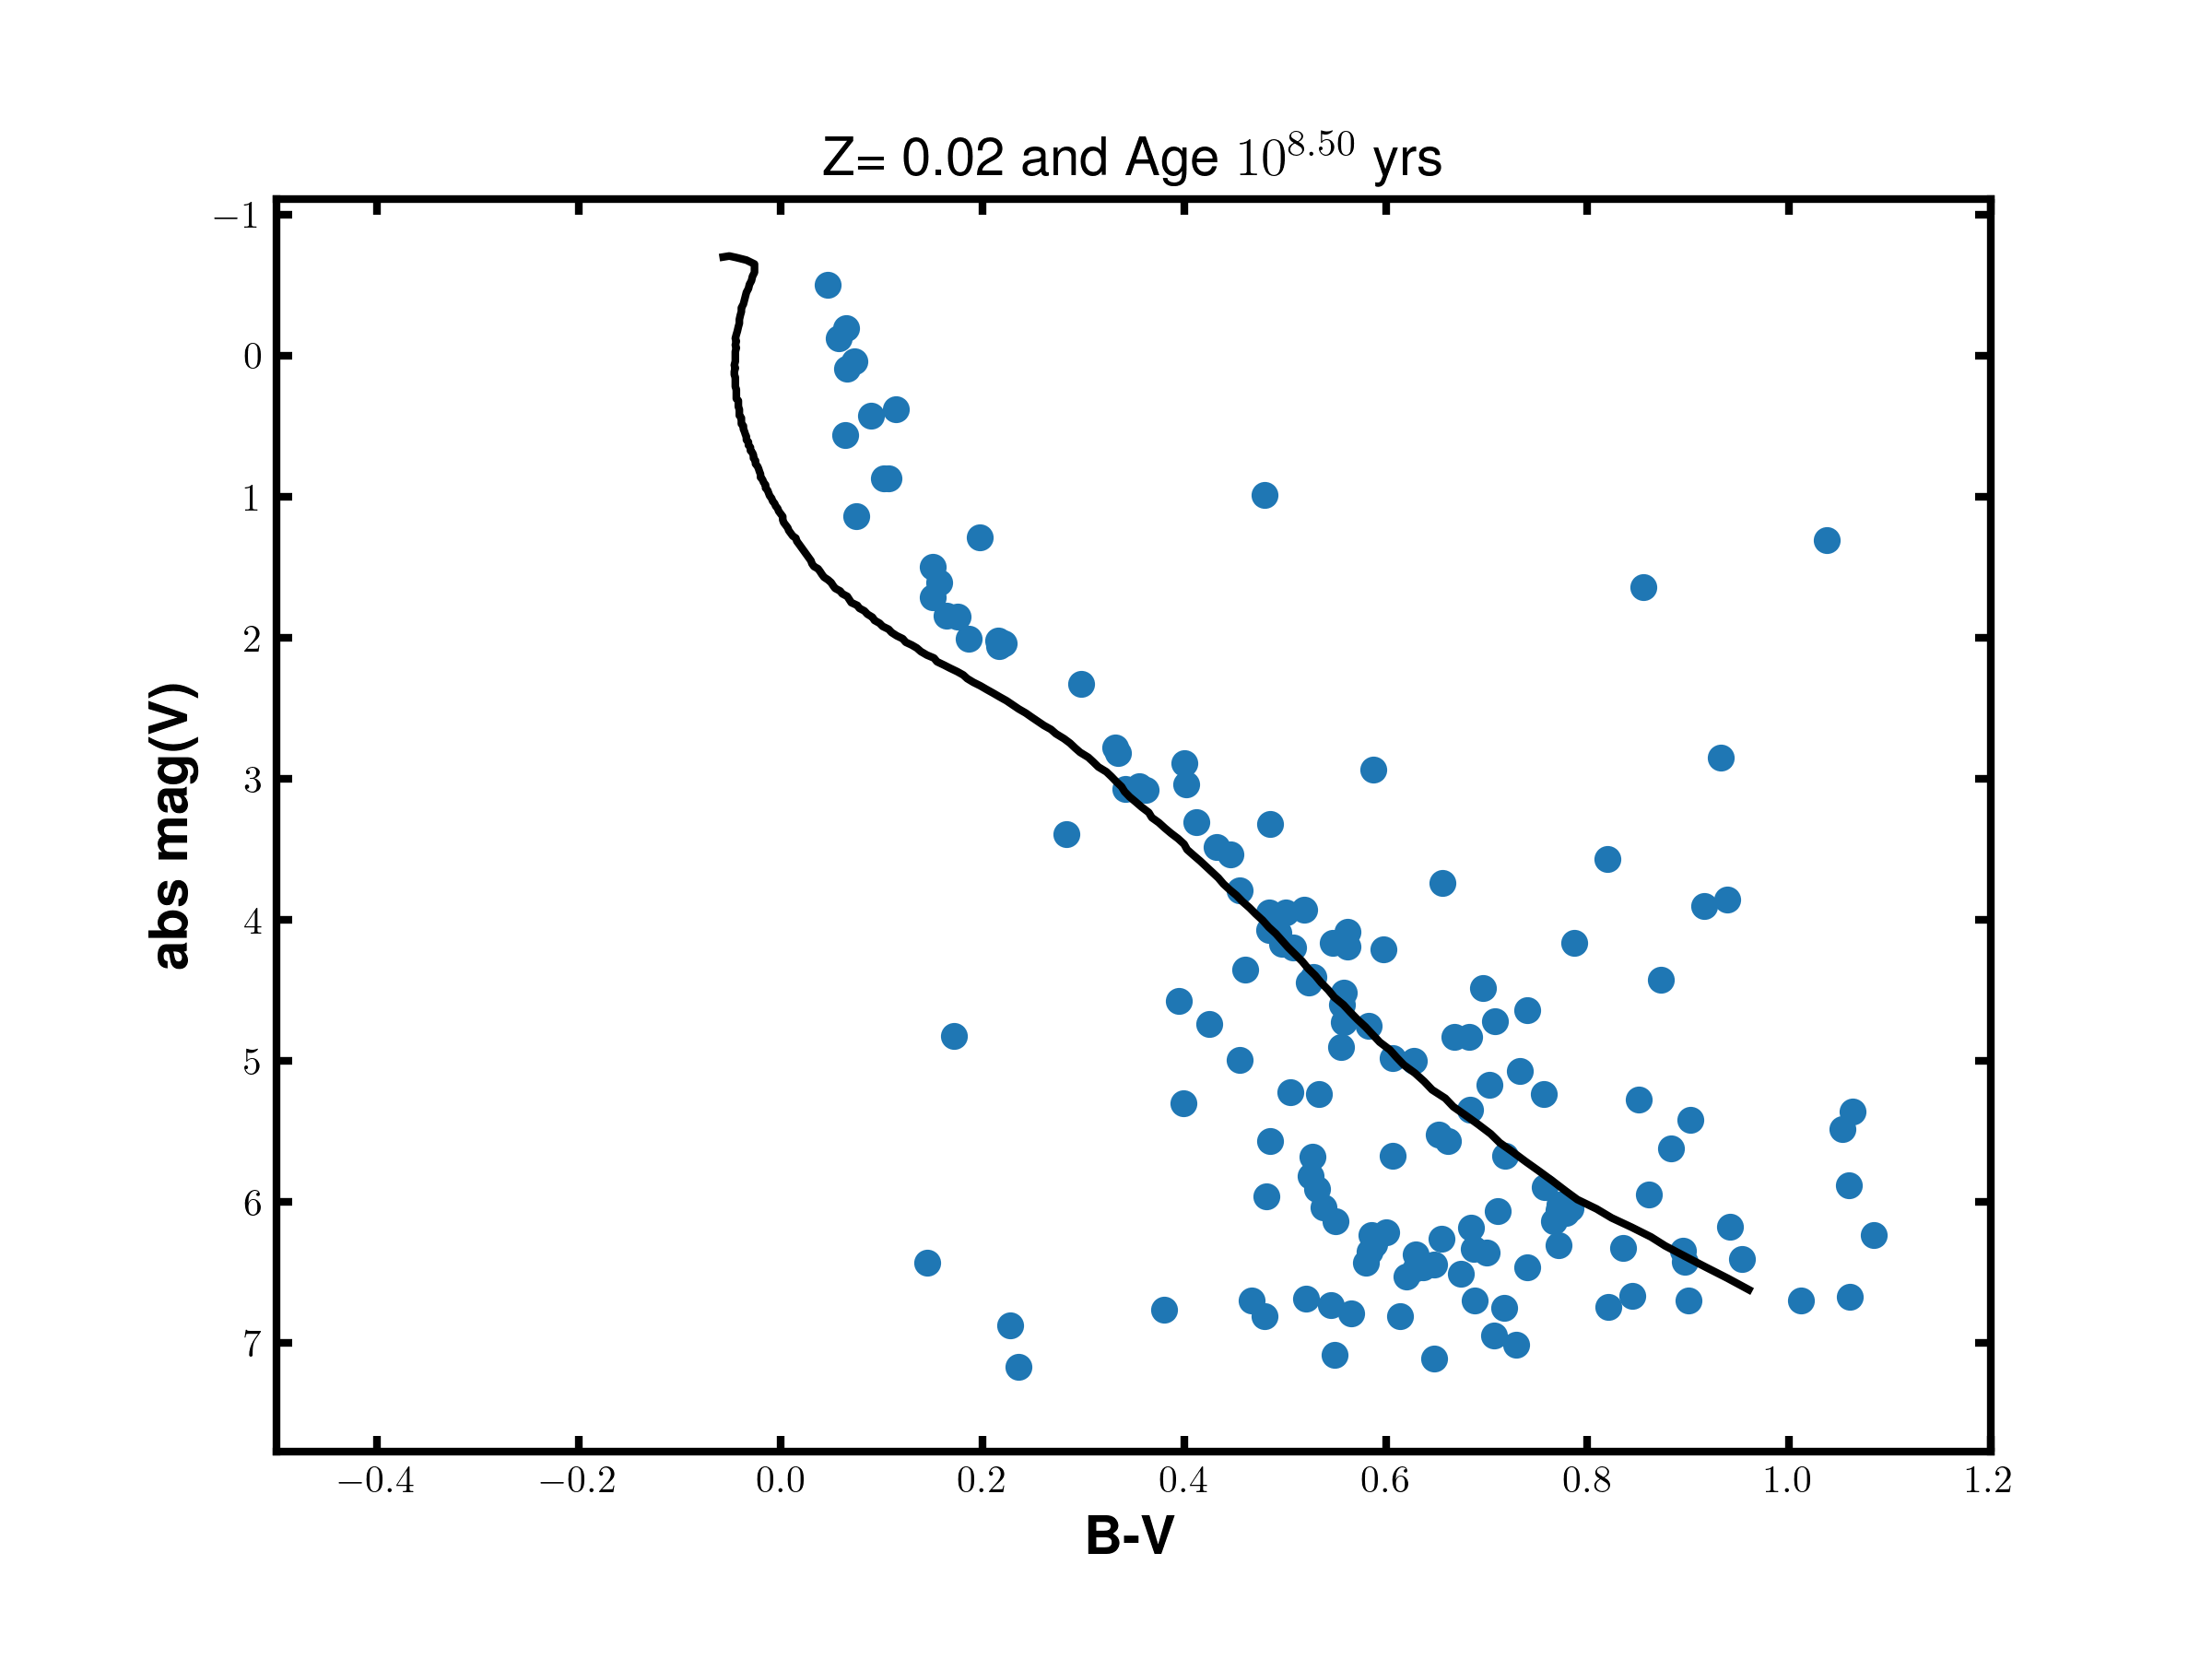
\includegraphics[width=\textwidth]{fig/iso_z020_850.png}
    \caption{CMD with the best isochrone fitted to the data}
    \label{isochrone}
\end{figure}

\begin{table}[H]
    \centering
    \begin{tabular}{c|c|c}
          \hline
          \hline
         Age [yr] & shift [mag] & Residuals [mag]  \\
         \hline
         $10^{8.55}$&8.38 &156.2649 \\
         $10^{8.35}$&8.37 &151.4967 \\
         $10^{8.39}$&8.37 &151.1395 \\
         $10^{8.44}$&8.38 &150.5916 \\
         $10^{8.50}$&8.38 &149.9542 \\
         \hline
    \end{tabular}
    \caption{Isochrones with the lowest residuals and Z=0.02}
    \label{tab1}
\end{table}

\subsection{Distance to the Cluster}
A distance to the cluster is calculated from a known distance modulus according to the following expression \cite{lecturenote}:

\begin{equation}
d \hspace{0.1cm} [\mathrm{pc}]=10^{0.2 \hspace{0.1cm} (m-M+5)} =10^{0.2 \hspace{0.1cm} (a+5)} 
\end{equation}
Where m is the apparent magnitude and M is the absolute magnitude. 
For a = $8.38 \pm 0.01$, we get a distance of d = $474 \pm 2 $ pc. This value is compatible with the literature value in Jones et al. \cite{jones} which gives d = 475 pc (no error given). 
\subsection{Age of the Cluster}
Following the analysis done, we obtain an age t = $10^{8.50} \simeq 316$ Myr. To approximate the error, we use the ages of the two closest isochrones since the ages of isochrones were more continuously distributed compared to the metallicities. This gives  t = $316^{+38}_{-41}$ Myr. This has a discrepancy of $0.4\%$ when compared to the value of t = $225 \pm 25$ Myr given in Jones et al. \cite{jones} and a discrepancy of $0.56\%$ compared to the value of t = $190 \pm 120$ Myr given in Netopil et al. \cite{netopil}. 

\subsection{Cluster Metallicity}
With the fitting done, we get a metallicity Z = $0.02 \pm 0.01$. The error added is due to our inability to narrow it down to metallicities. 

\section{Discussion}
A large scatter of data points around the isochrone is realized in Figure \ref{isochrone}. This wide spread of points could be due to multiple factors. First, the creation of isochrones could be done under very simplified assumptions. For example, the assumption of the formation of a cluster from a homogenous cloud. As a result, any non-considered inhomogeneity leads to a change of positions of data points in the CMD as metalicity and temperature change (e.g. having binary systems or peculiar stars). Second, what can change the positions of stars in the CMD is the time of their formation. For instance, if stars form at different stages of evolution instead of being created at the same time, a wider variance of positions on the CMD can be realized. 
We get an age that deviates from literature values. This is because the determination of the age is highly dependent on the precise calibration of B and V measurements. Given that we did not have the benefit of observing a reference star and relied on data from only 25 stars, it is reasonable to expect a relatively large margin of error in our estimate of the cluster's age.
Finally, the discrepancy in the obtained value of metallicity can be reduced with a larger number of SCIENCE frames taken. 

\section{Conclusion}
In this laboratory, we observe an open cluster M34 and determine its age, distance and metallicity by constructing a color magnitude diagram. We process raw images taken from a 50 cm Cassegrain telescope on the rooftop at the Argelander-Institut
für Astronomie at the University of Bonn. Multiple image processing steps are taken to produce reduced science frames. Then, calibration is done construct a CMD diagram. Furthermore, we fit isochrones from a data set to the CMD and determine the age to be t = $316^{+38}_{-41}$ Myr, metallicity to be Z = 0.02. and the distance to be $d = 474 \pm 2 \mathrm{pc}$ .  We describe potential error in the data in the discussion section. Multiple steps can be taken to improve the data: Reducing the number of false detections, applying more sophisticated fitting models to the isochrones and also reducing the number of assumptions used in the manual to conduct the analysis. 

\printbibliography

\appendix
\section*{Appendix}
\section{Figures}\label{append}

    \begin{figure}[H]
    \centering
    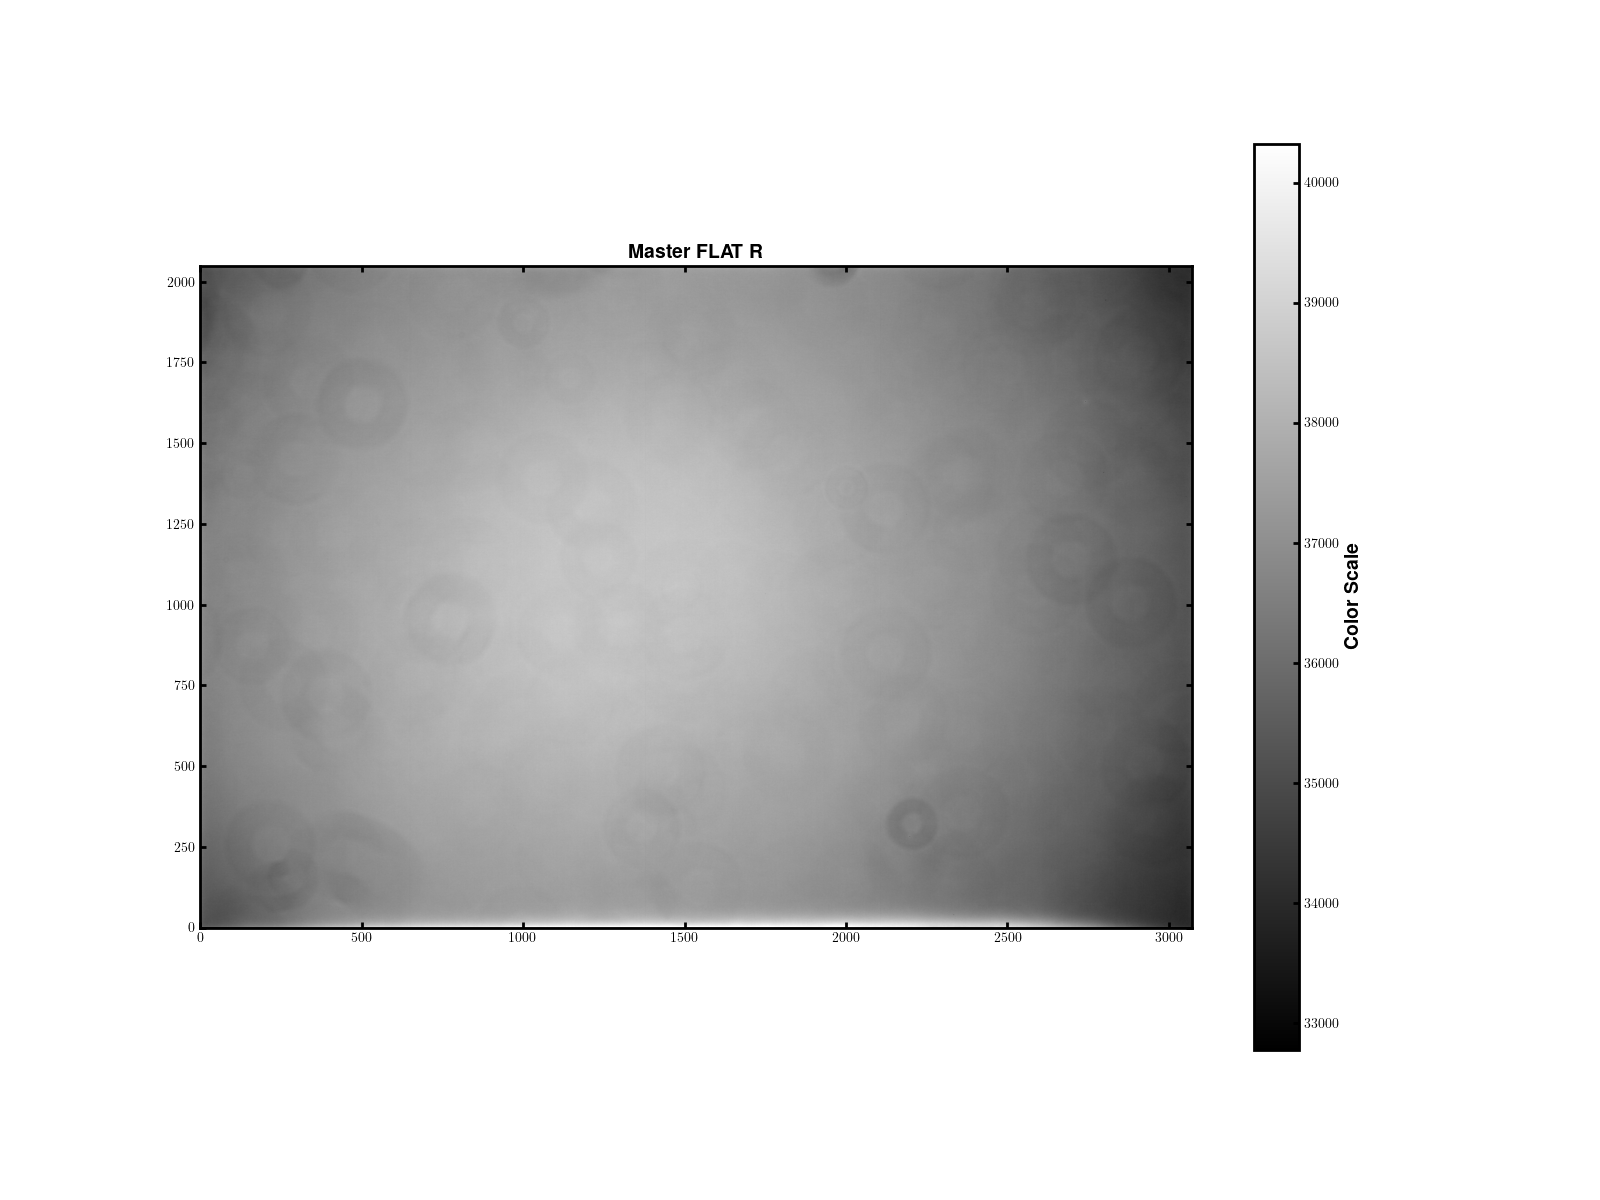
\includegraphics[width=\textwidth]{fig/Master_FLAT_R.png}
    
    \caption{MASTER FLAT Frame in R band}
    \end{figure}

    \begin{figure}[H]
    \centering
    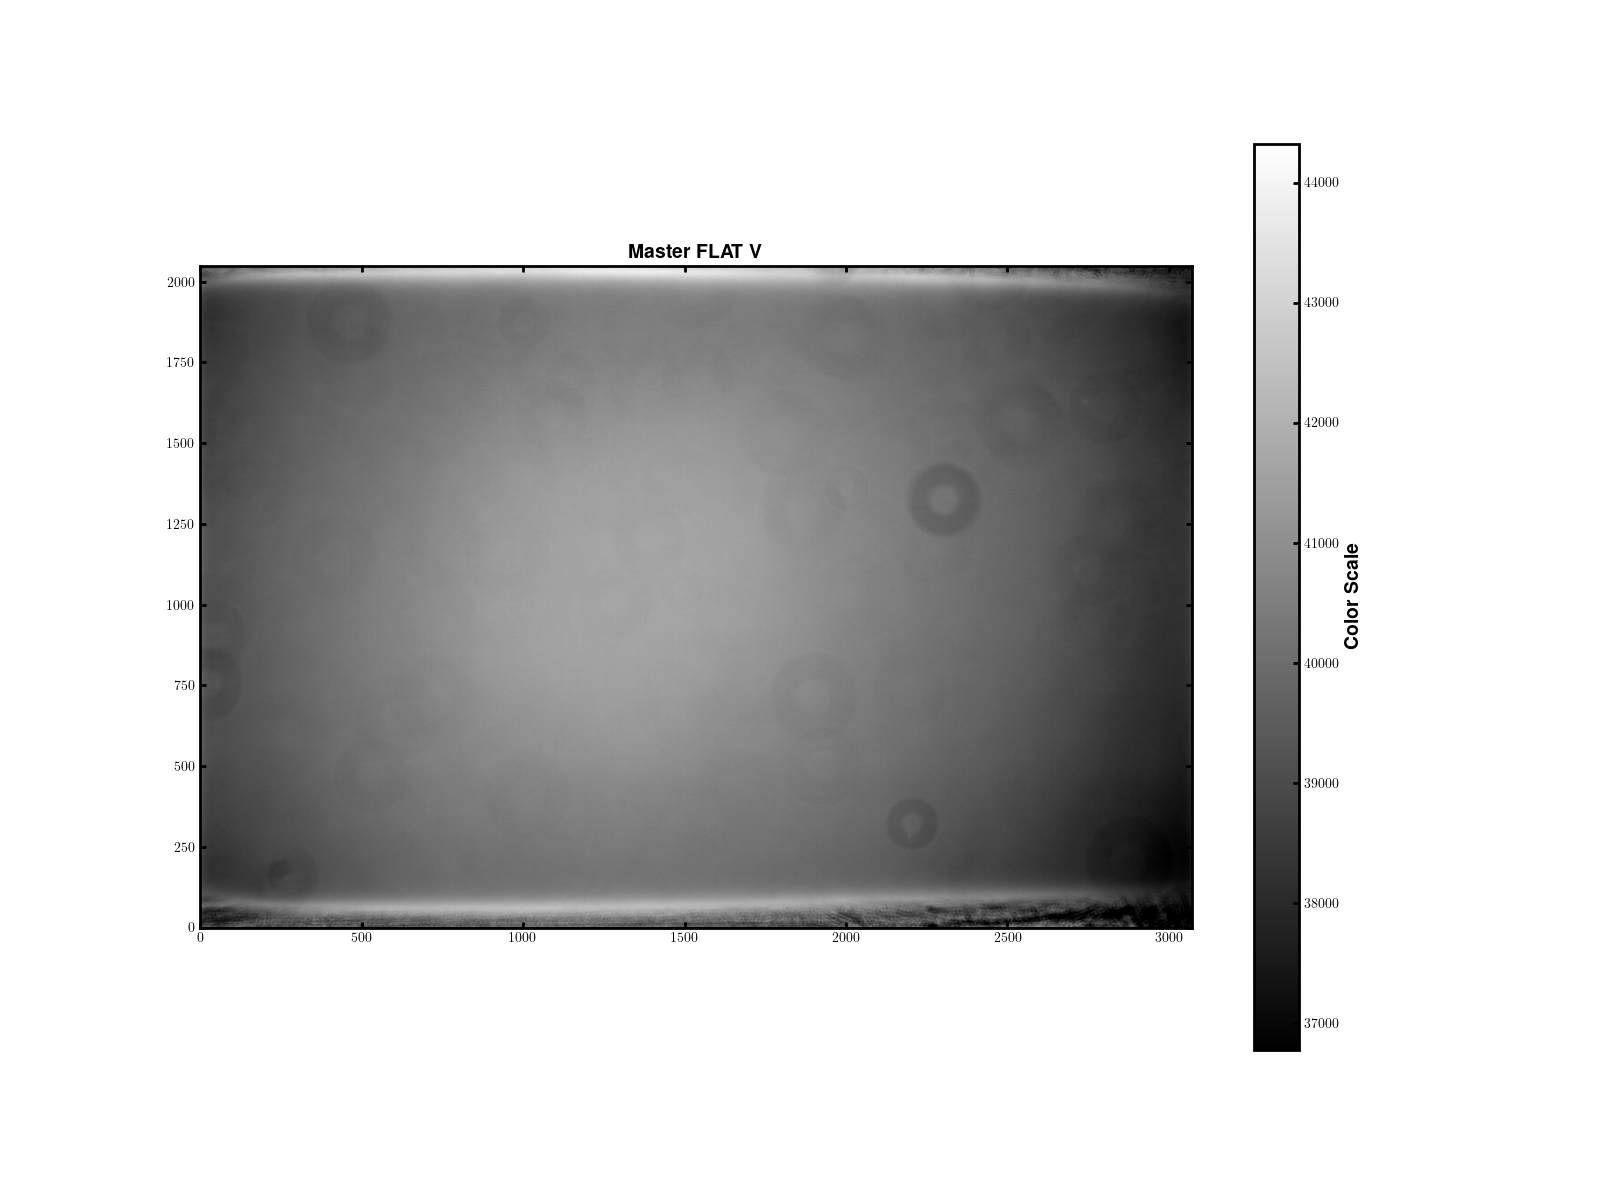
\includegraphics[width=\textwidth]{fig/Master_FLAT_V.png}
    
    \caption{MASTER FLAT Frame in V band}
    \end{figure}

    \begin{figure}[H]
    \centering
    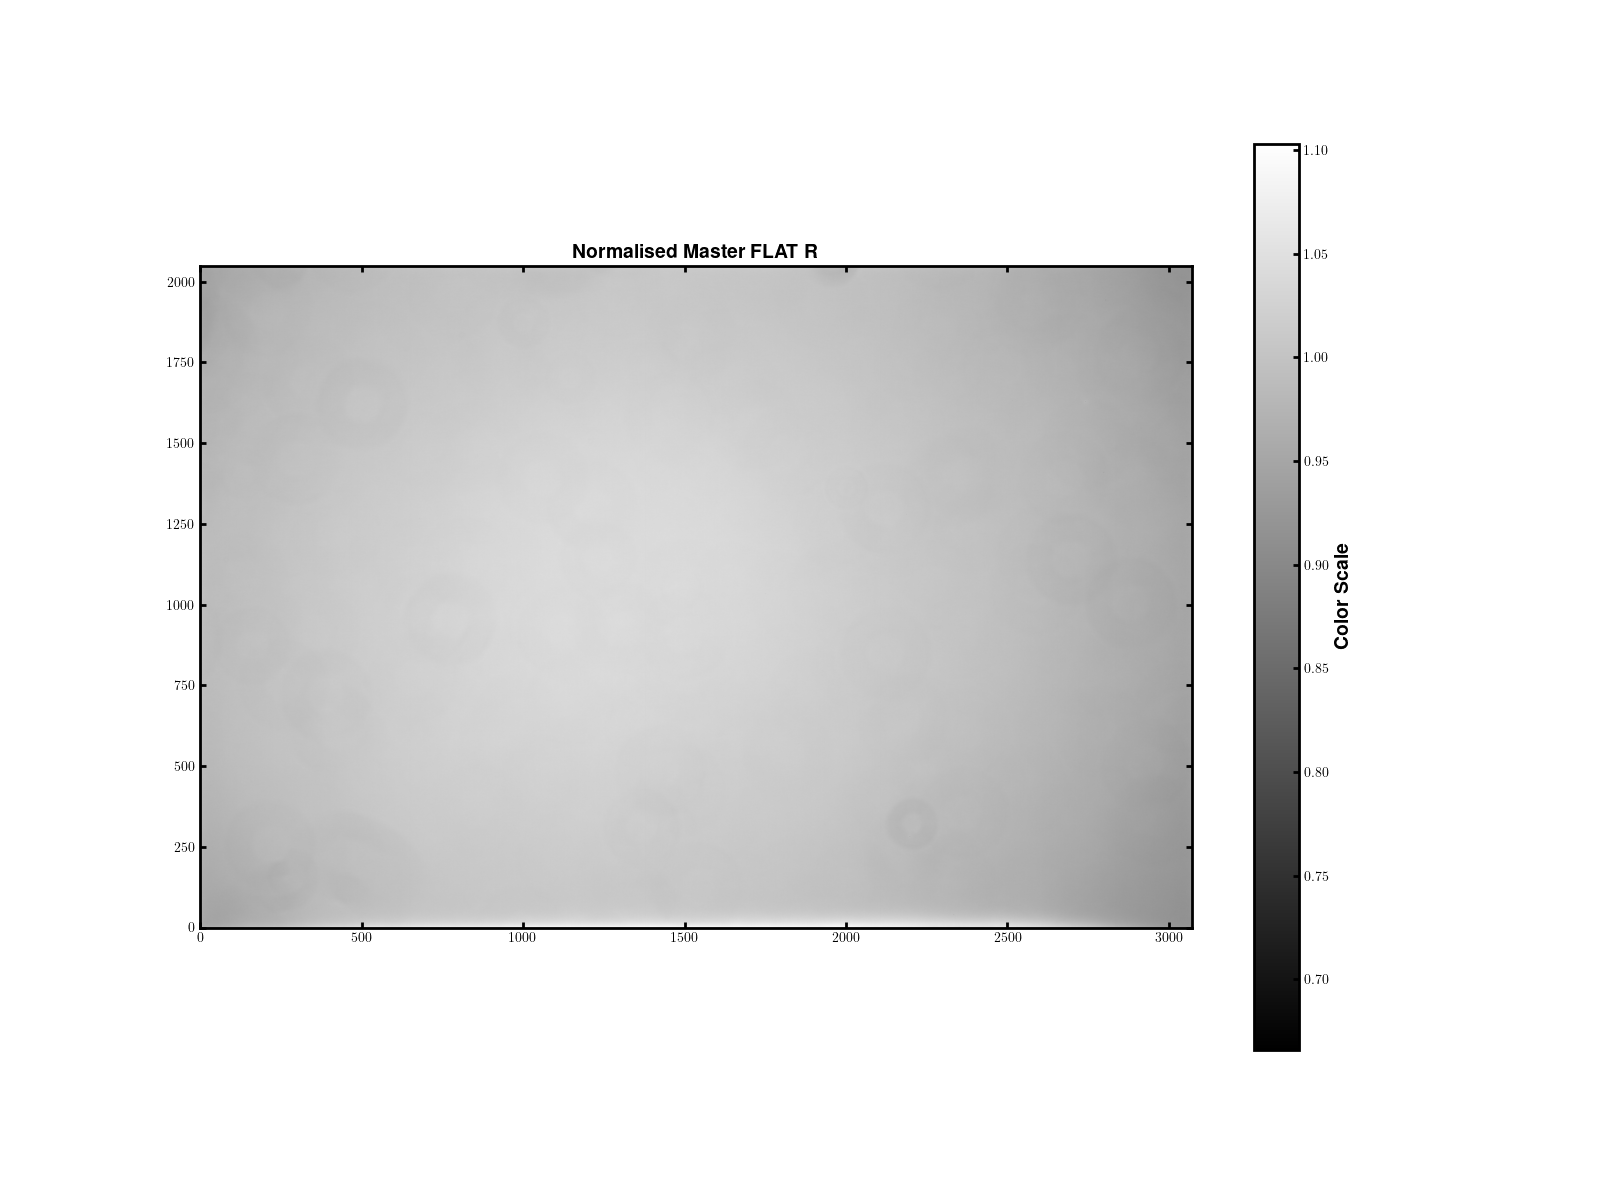
\includegraphics[width=\textwidth]{fig/Normal_Master_FLAT_R.png}
    \caption{Normalized MASTER FLAT frame in the R band}

    \end{figure}

    \begin{figure}[H]
    \centering
    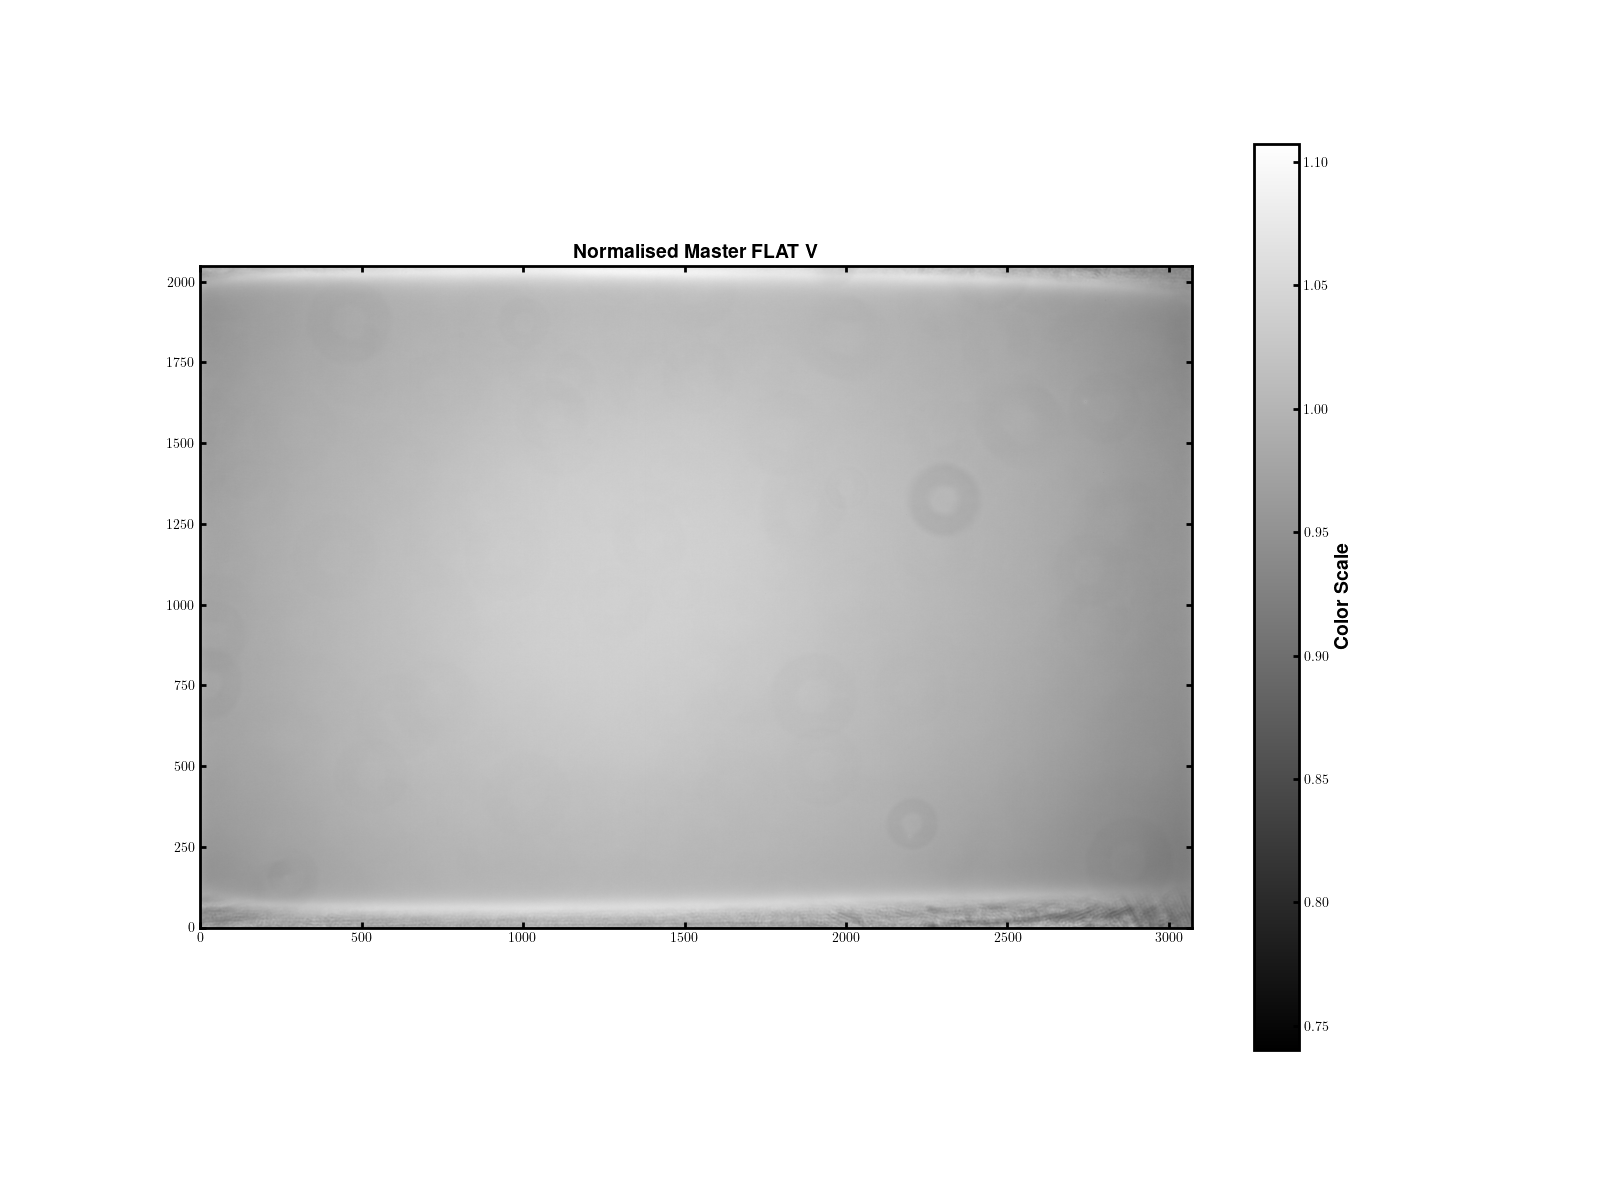
\includegraphics[width=\textwidth]{fig/Normal_Master_FLAT_V.png}
    \caption{Normalized MASTER FLAT frame in the v band}

    \end{figure}


    \begin{figure}[H]
    \centering
    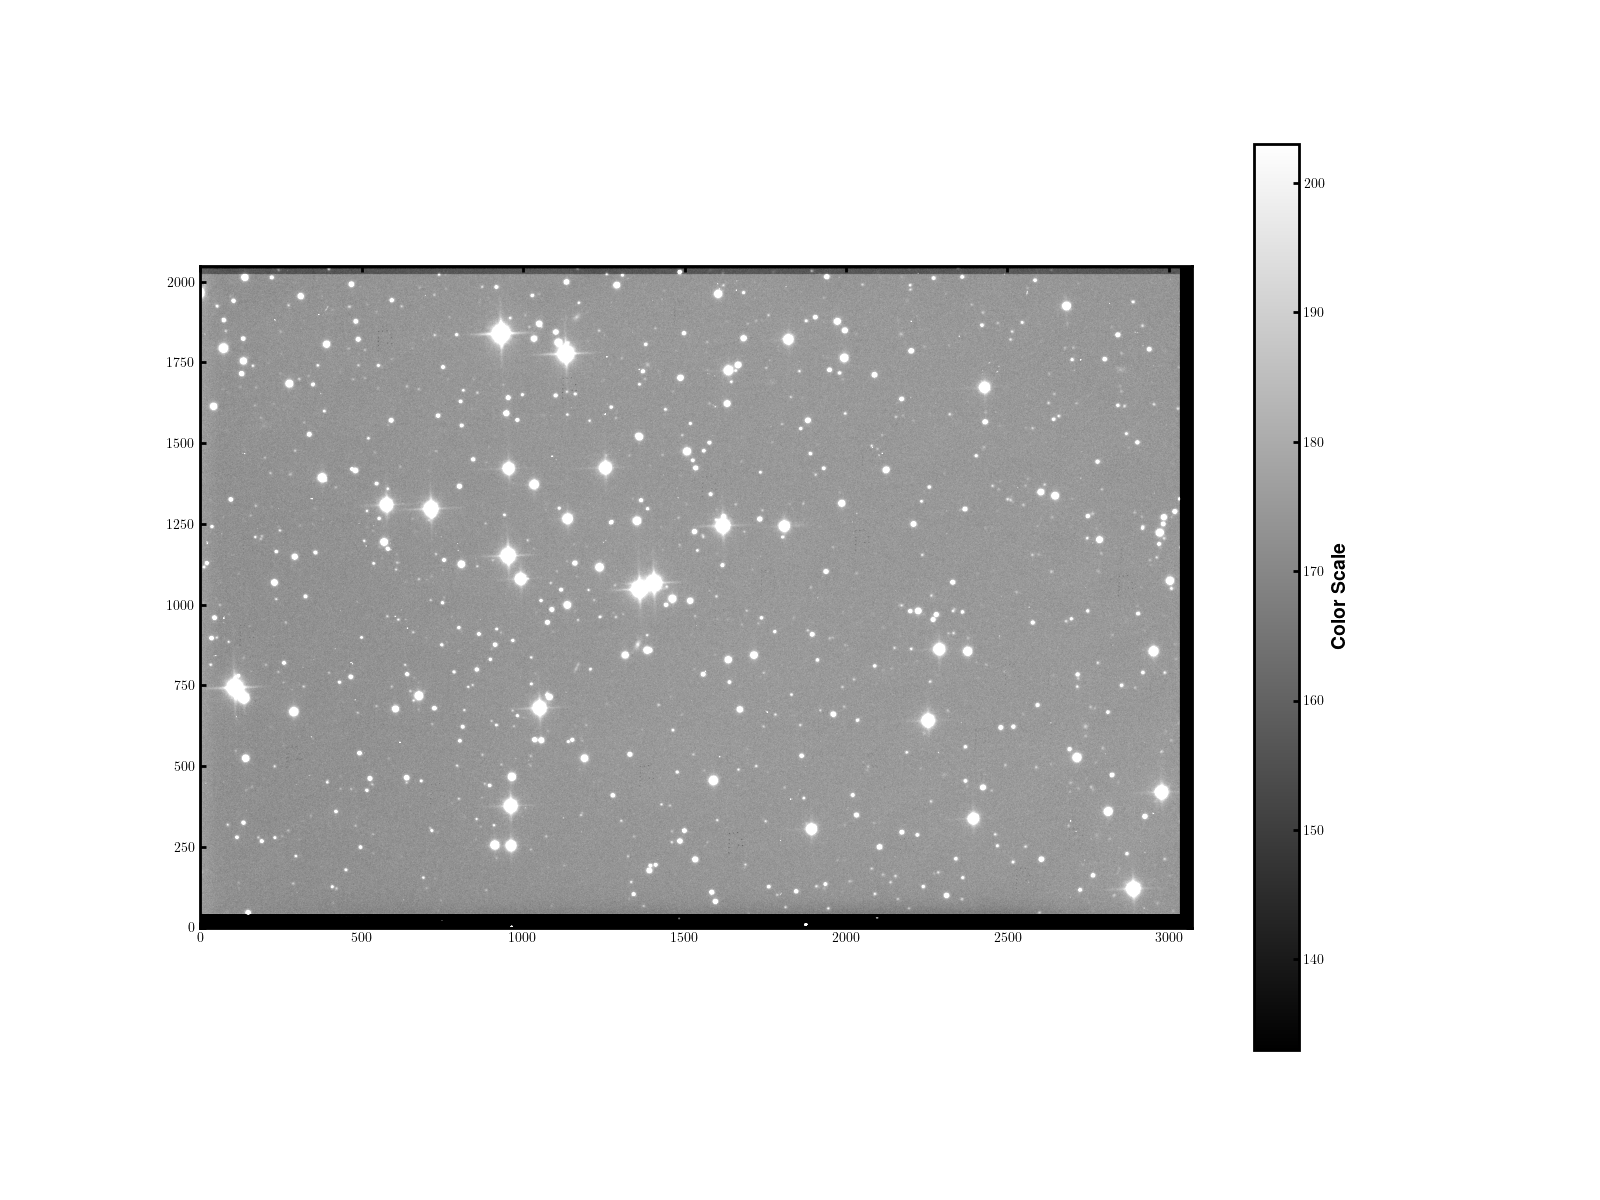
\includegraphics[width=\textwidth]{fig/Co-added_reduced_master_R.png}
    \caption{ Co-added reduced master science frame in the R-band}

    \end{figure}

    \begin{figure}[H]
    \centering
    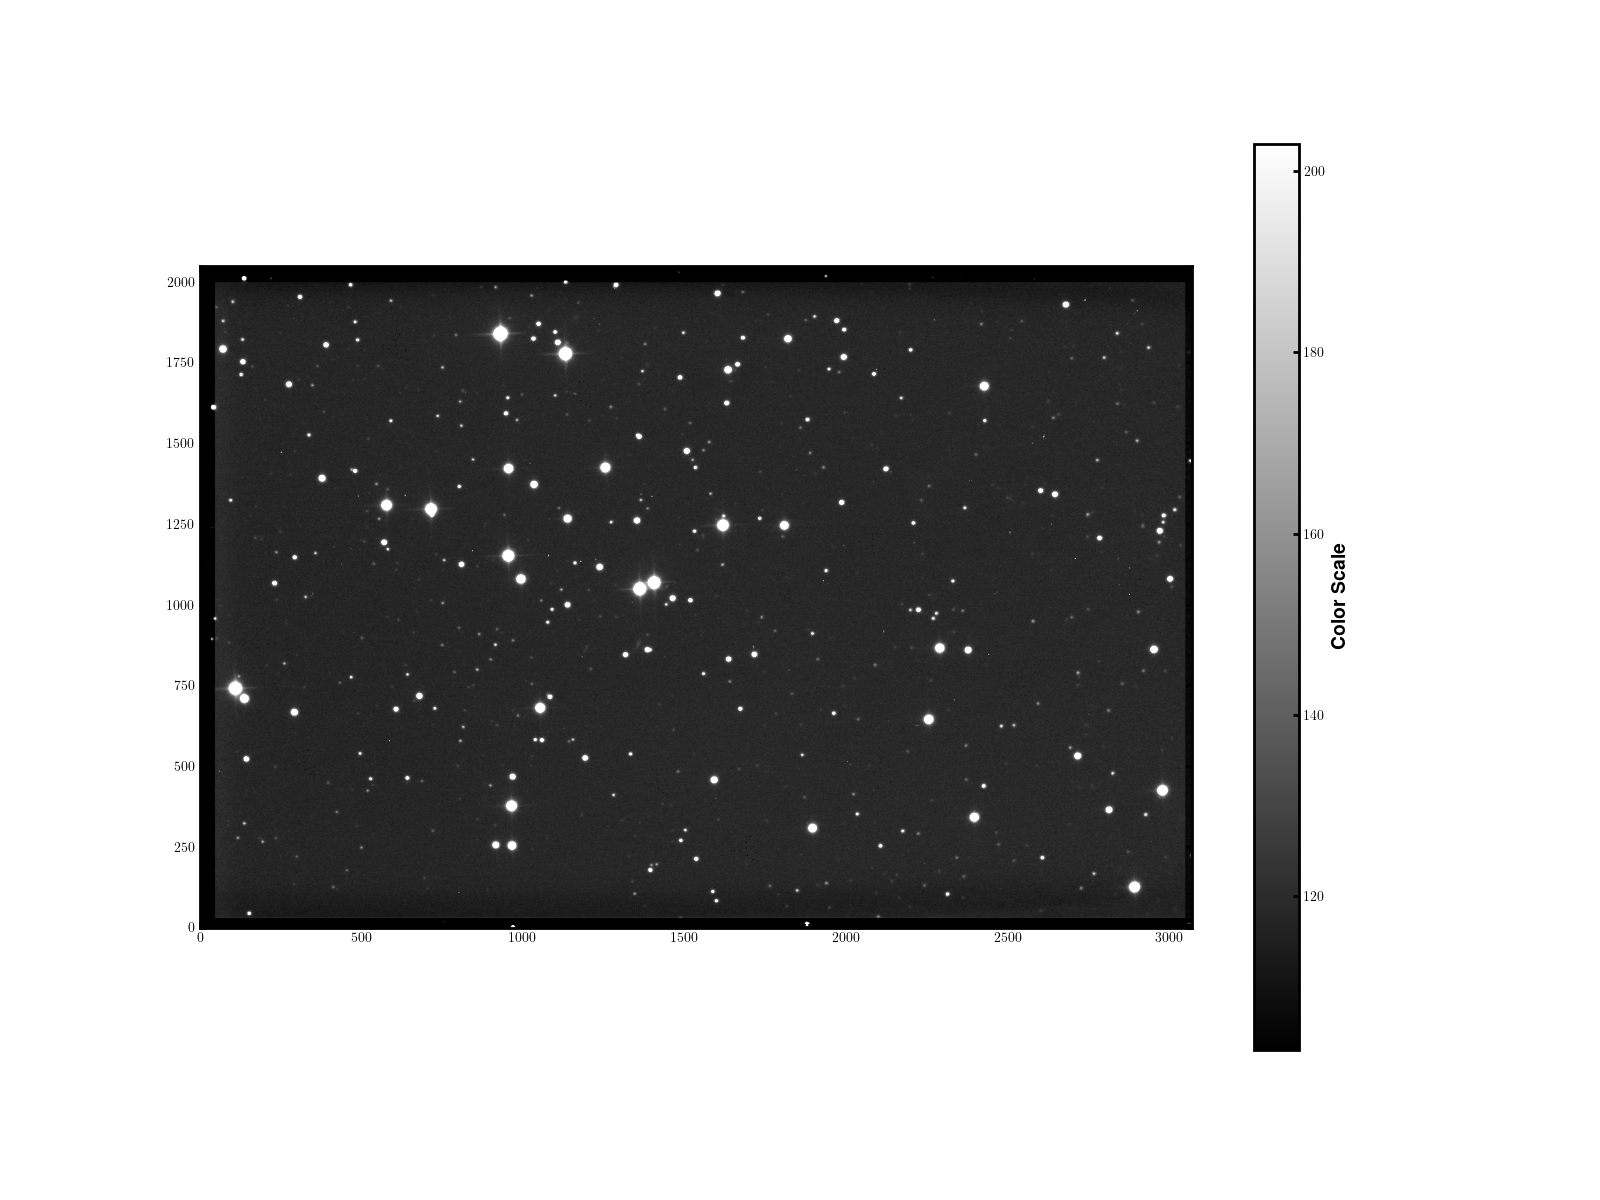
\includegraphics[width=\textwidth]{fig/Co-added_reduced_master_V.png}
    \caption{ Co-added reduced master science frame in the V-band}

    \end{figure}

    \begin{figure}[H]
    \centering
    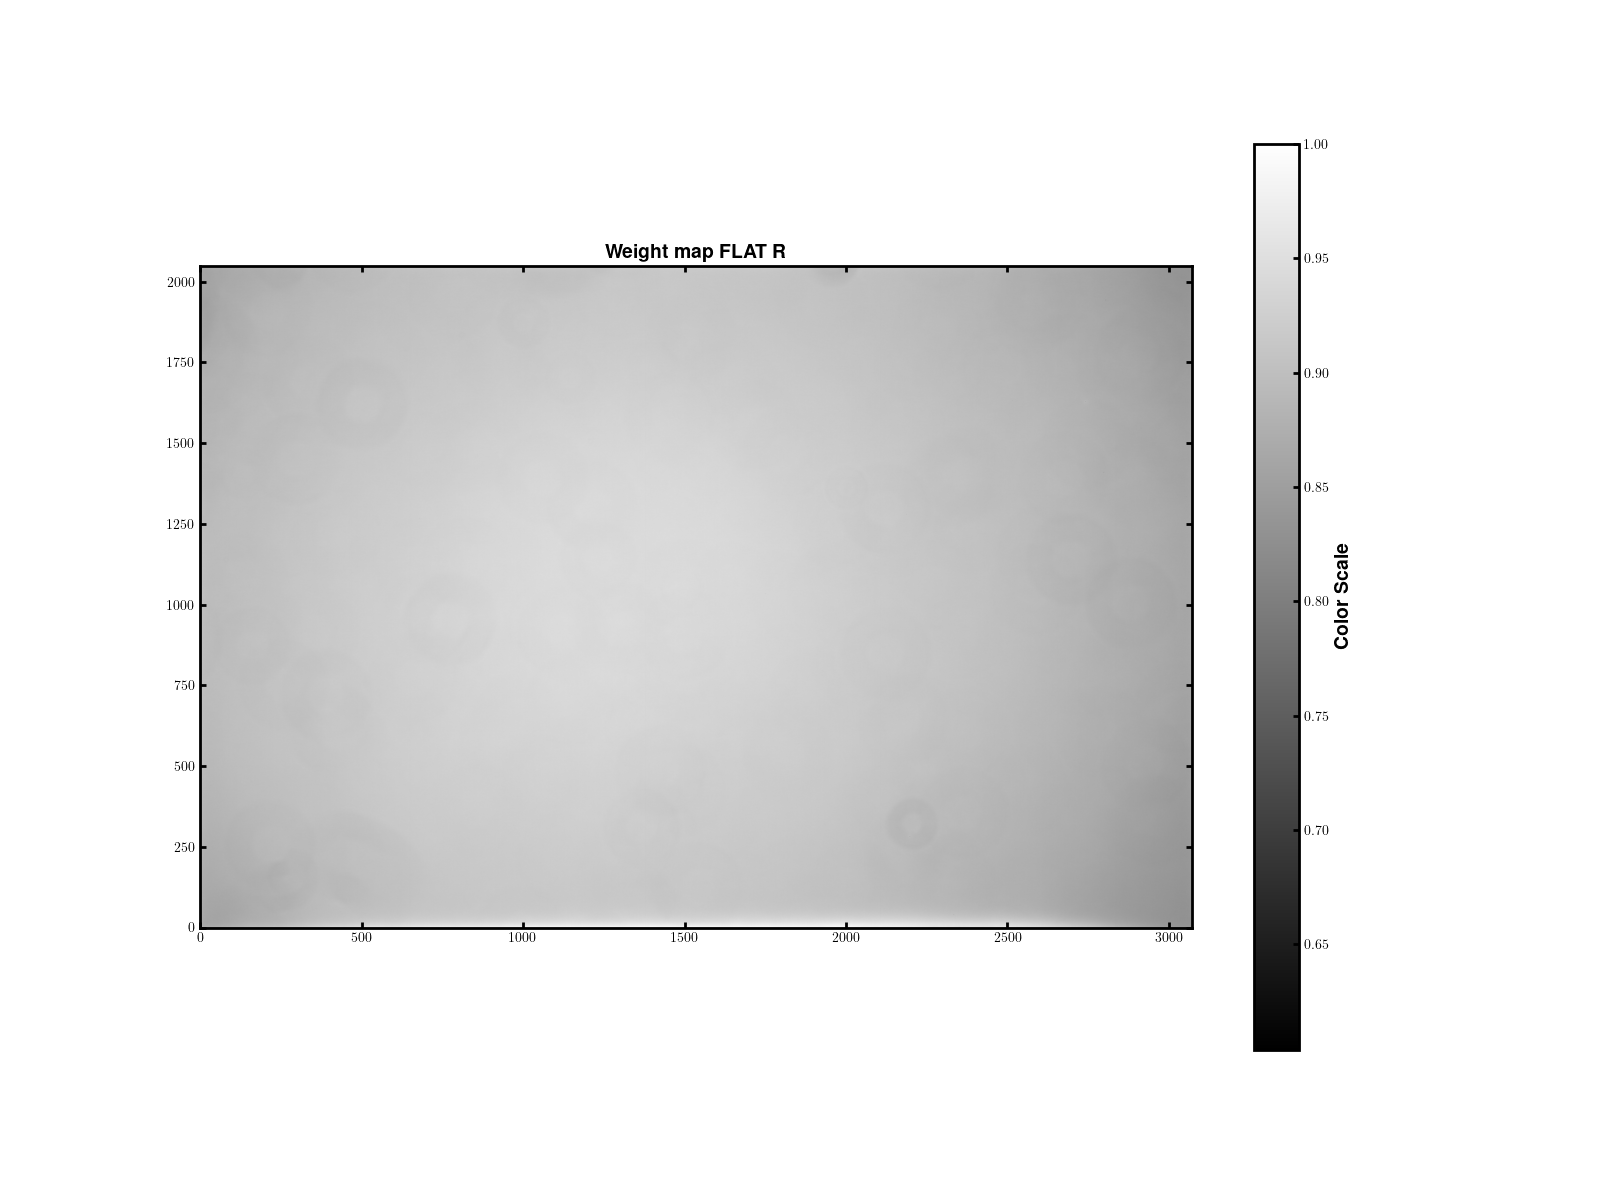
\includegraphics[width=\textwidth]{fig/weightmap_FLAT_R.png}
    \caption{ Weighted master flat frame in the R-band}

    \end{figure}

    \begin{figure}[H]
    \centering
    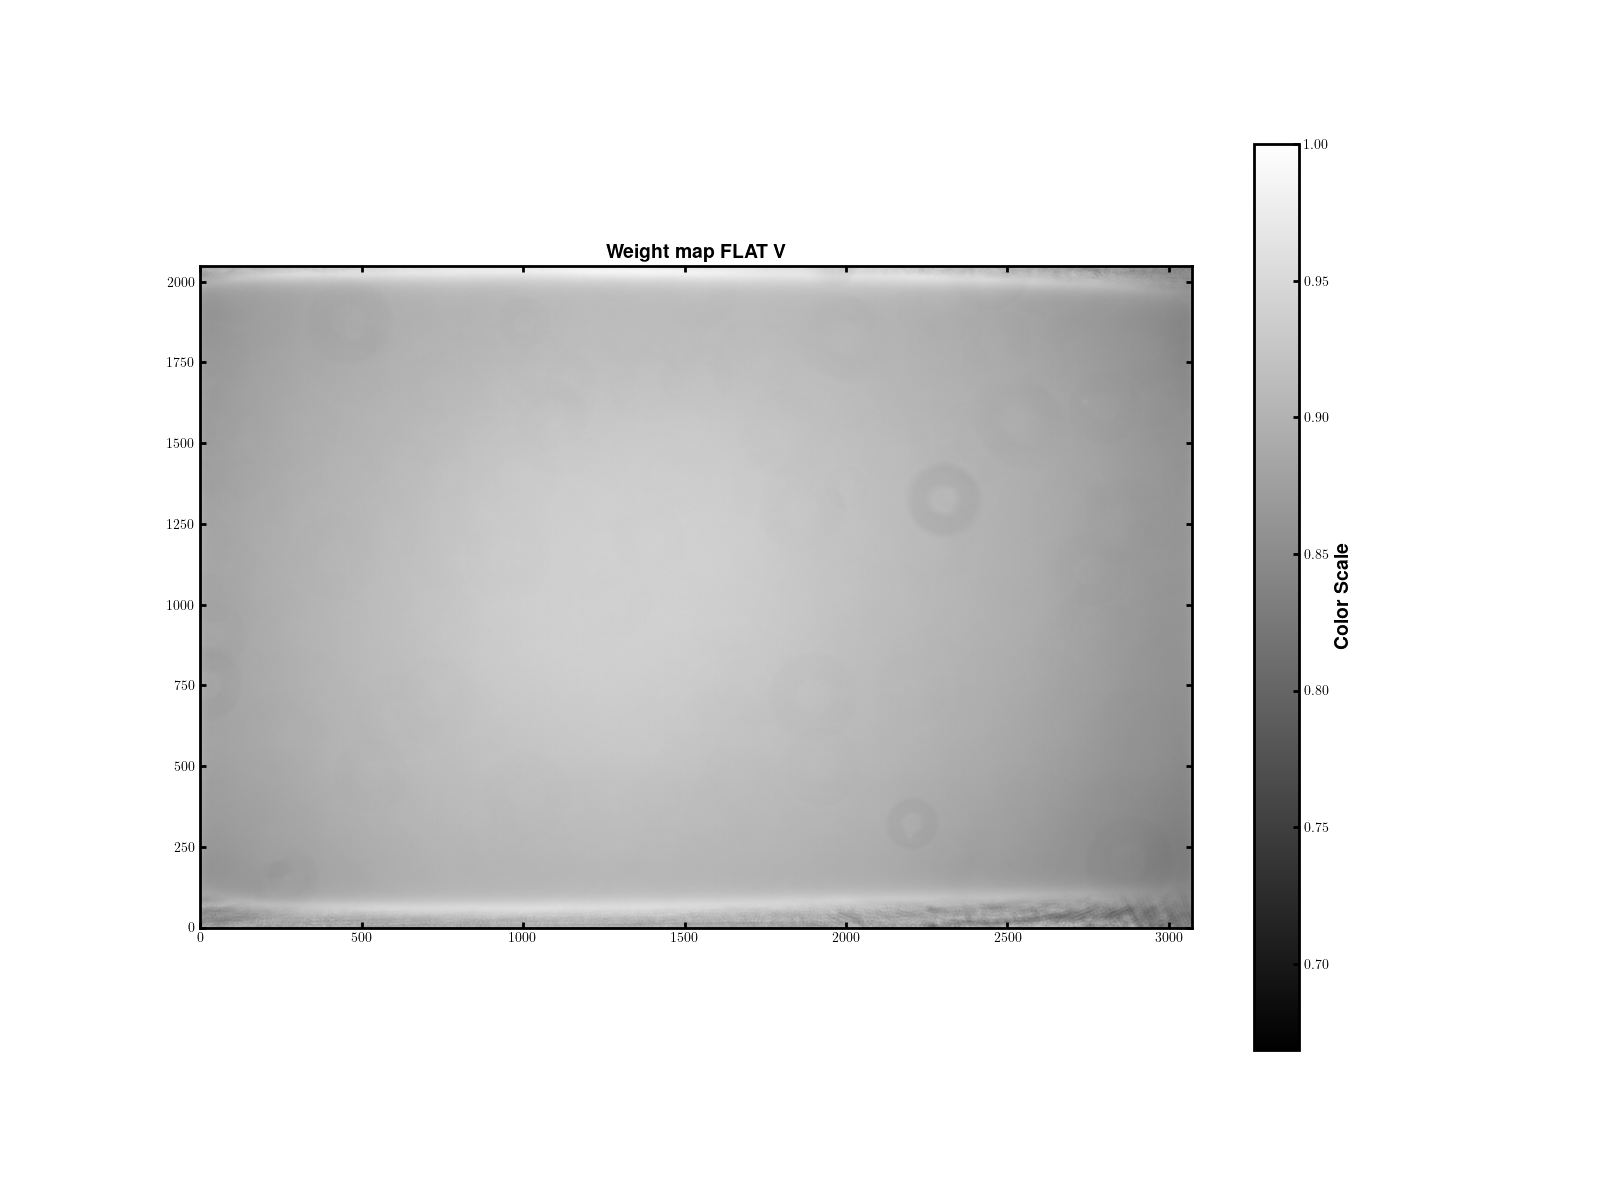
\includegraphics[width=\textwidth]{fig/weightmap_FLAT_V.png}
    \caption{ Weighted master flat frame in the V-band}

    \end{figure}

    \begin{figure}[H]
    \centering
    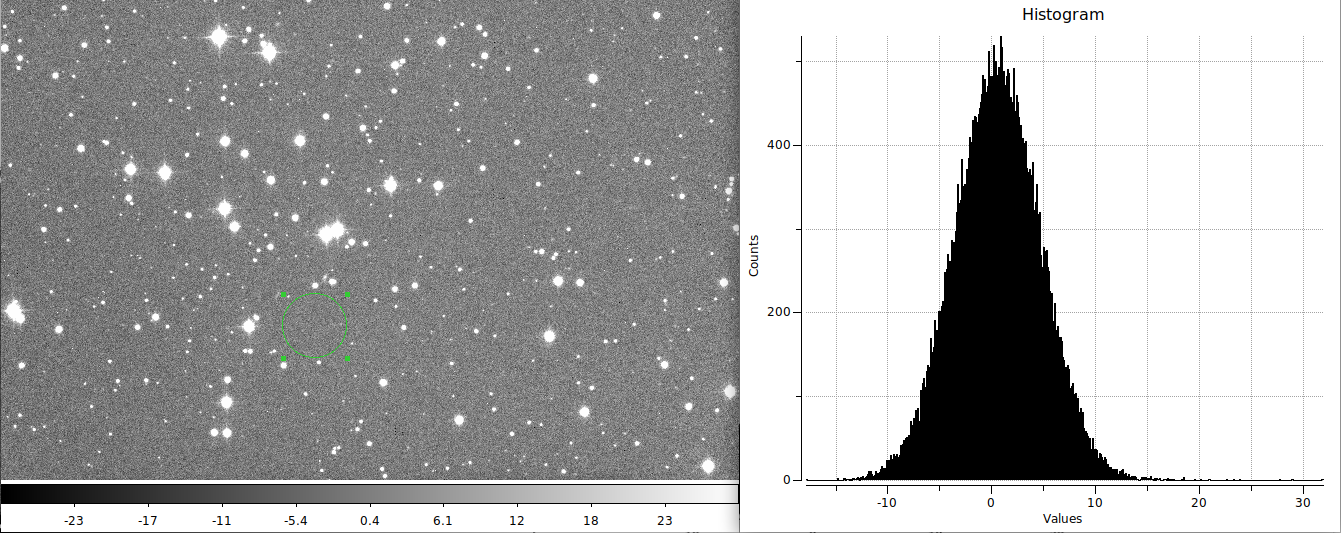
\includegraphics[width=\textwidth]{fig/backsub_R.png}
    \caption{Left: Background subtracted reduced master science frame in the R band. Right: Histogram of background region}

    \end{figure}

    \begin{figure}[H]
    \centering
    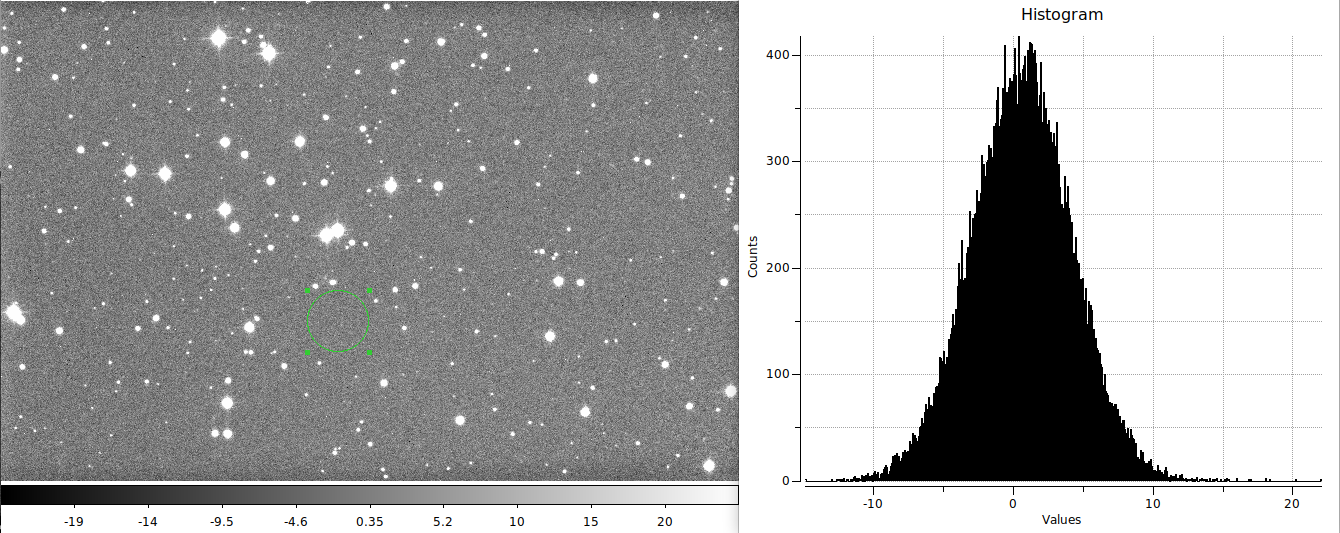
\includegraphics[width=\textwidth]{fig/backsub_V.png}
    \caption{Left: Background subtracted reduced master science frame in the v band. Right: Histogram of background region}

    \end{figure}

    \begin{figure}[H]
    \centering
    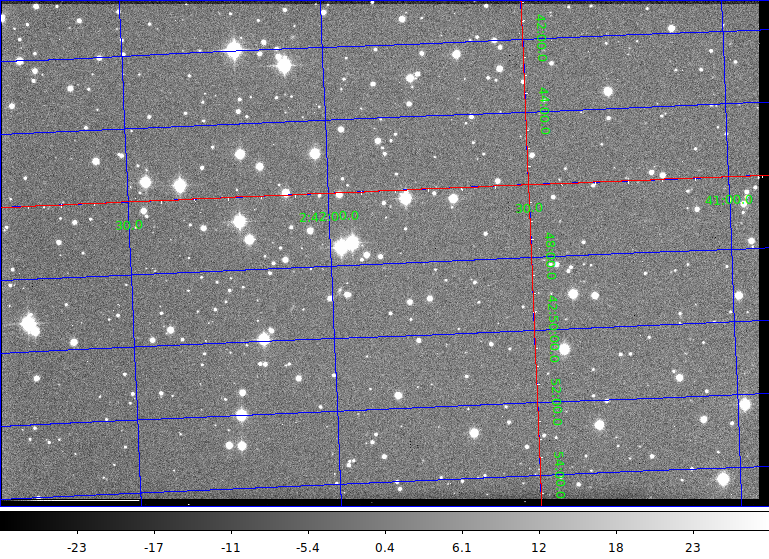
\includegraphics[width=\textwidth]{fig/Astrometric_Calibration_R.png}
    \caption{An astrometric Background-Subtracted Image in the R band}

    \end{figure}

    \begin{figure}[H]
    \centering
    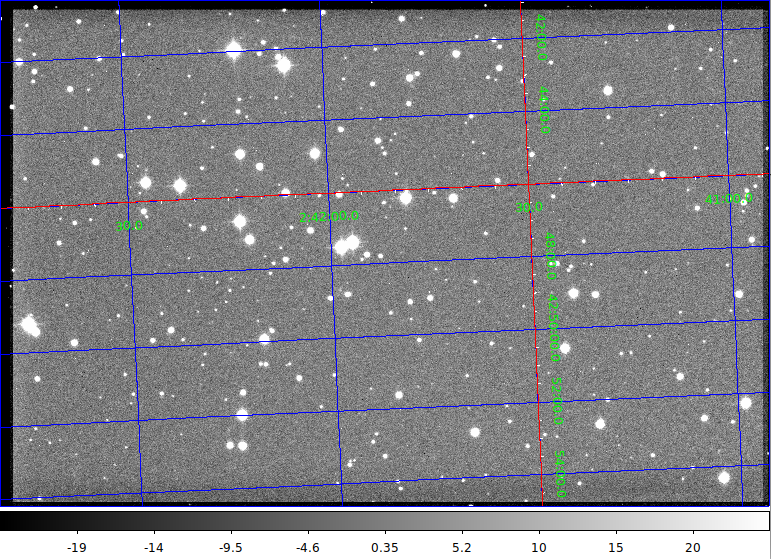
\includegraphics[width=\textwidth]{fig/Astrometric_Calibration_V.png}
    \caption{An astrometric Background-Subtracted Image in the V band}

    \end{figure}

    \begin{figure}[H]
    \centering
    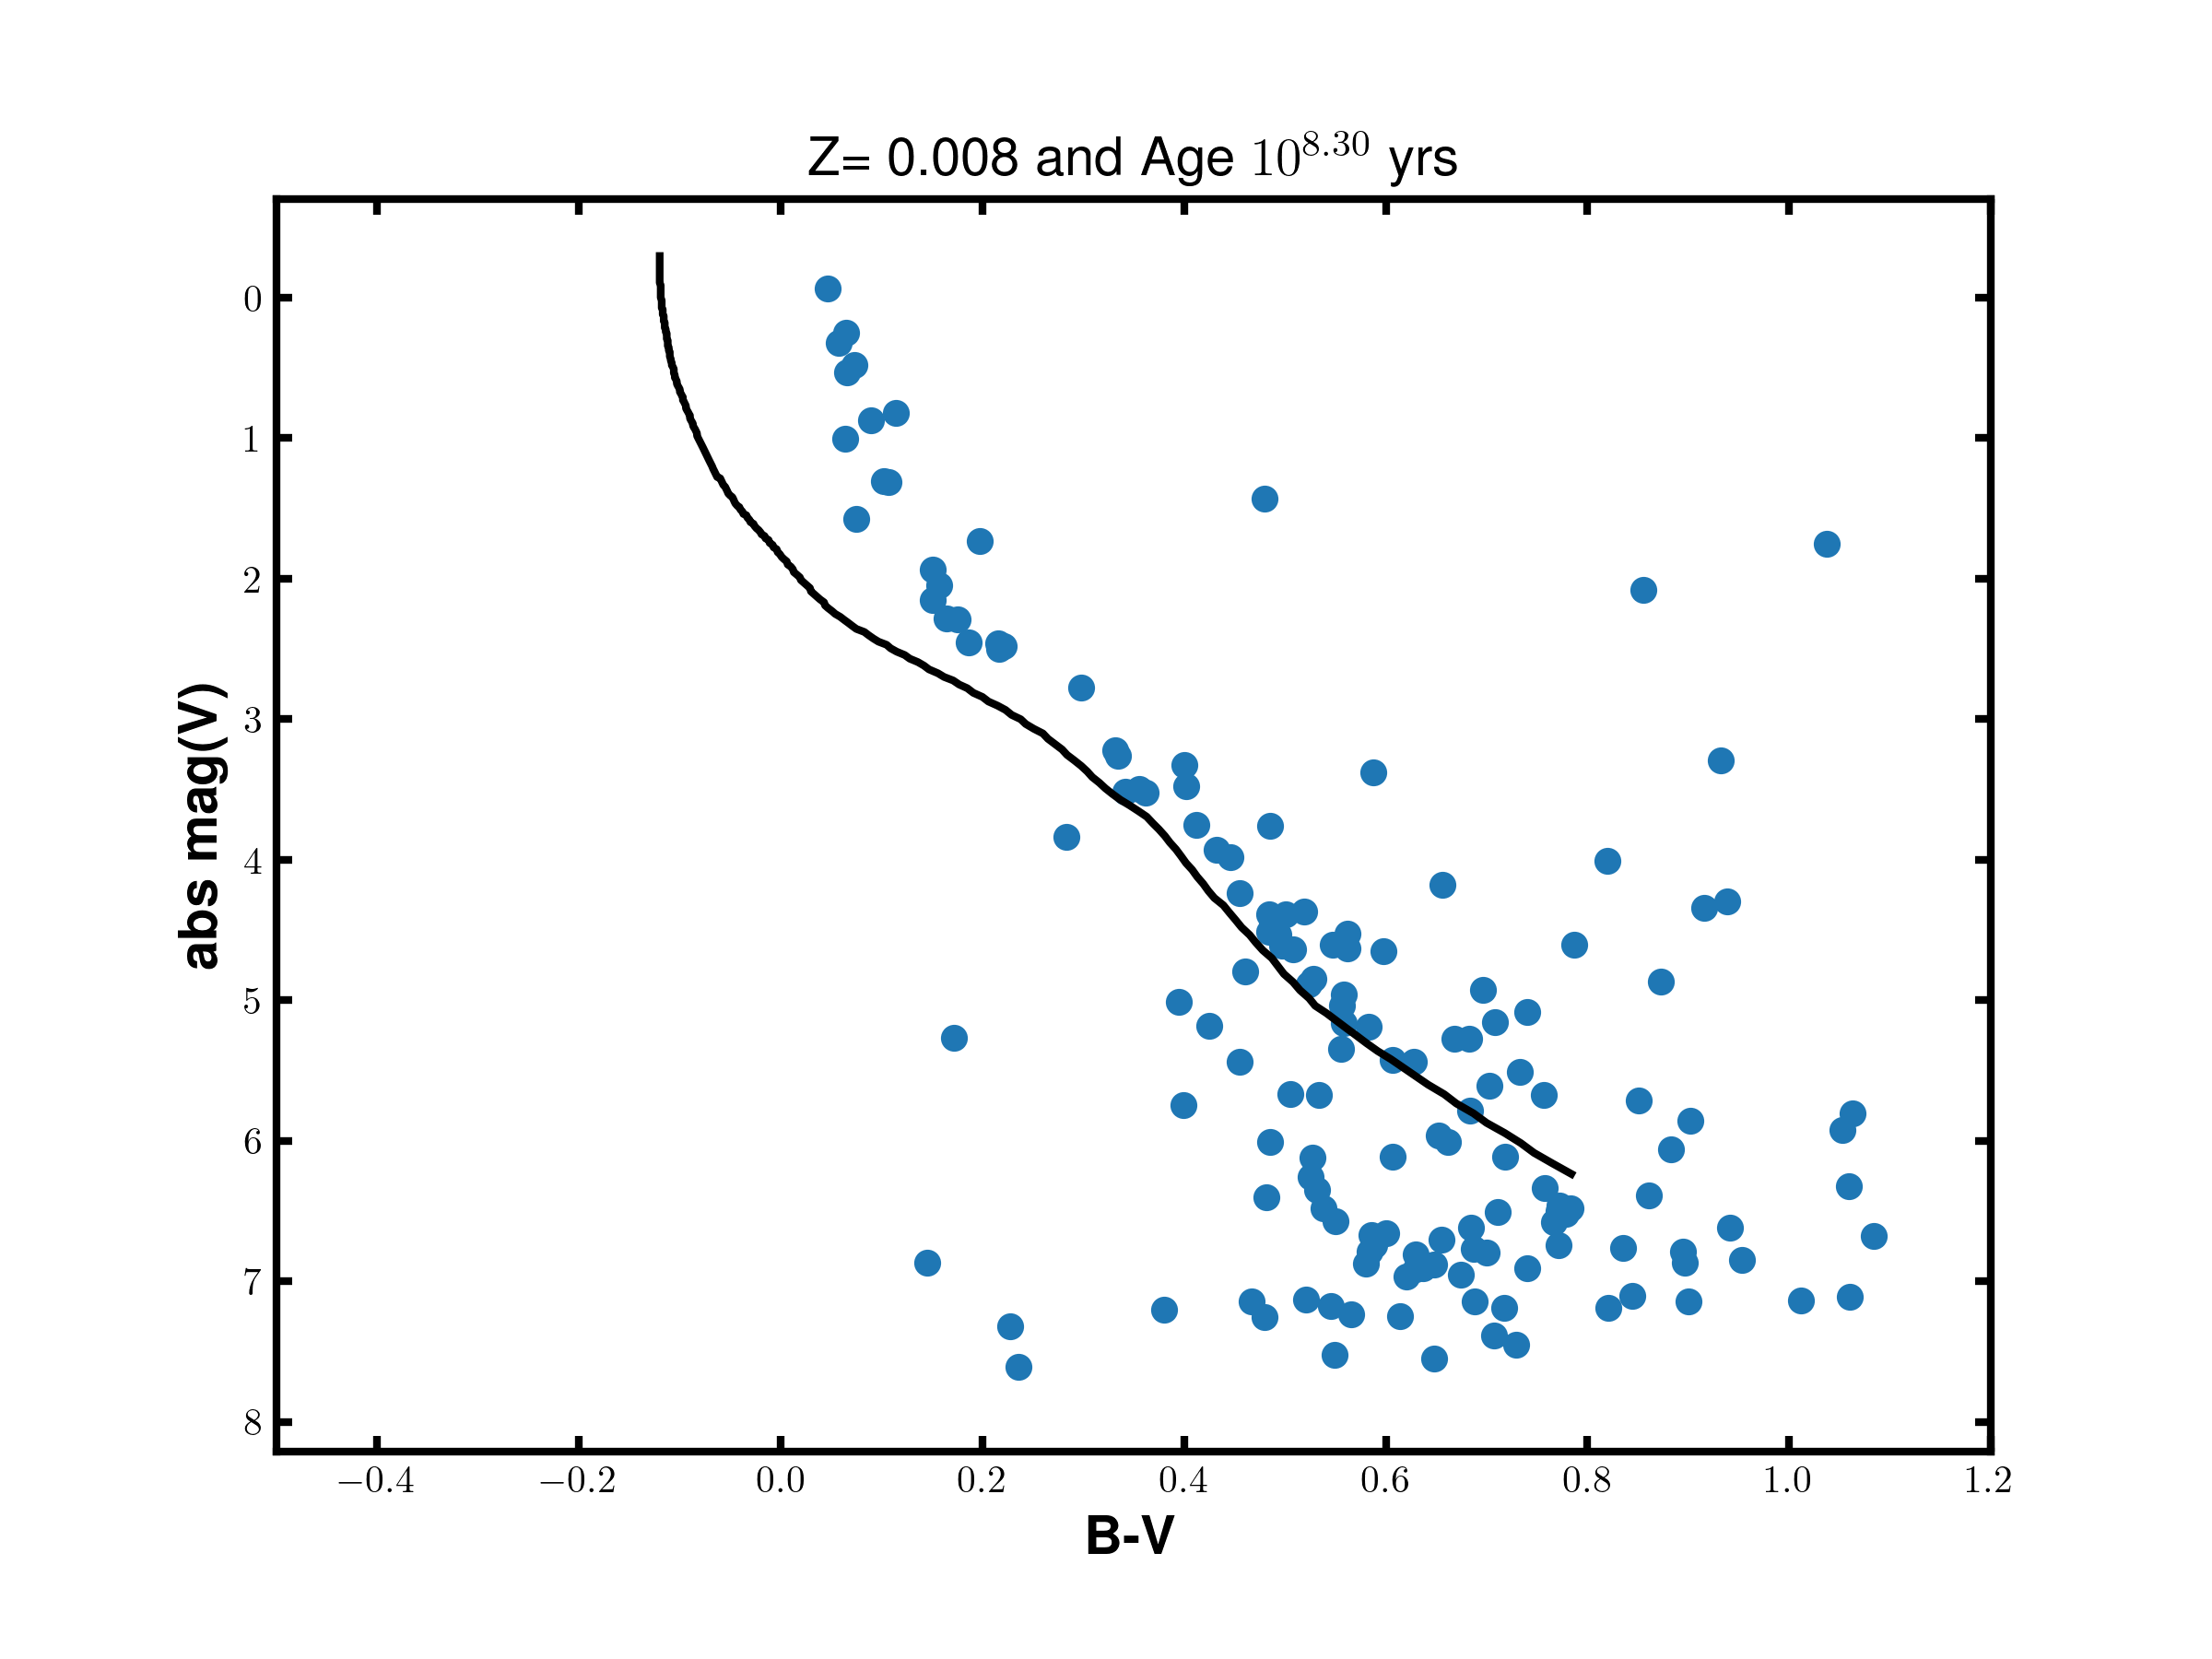
\includegraphics[width=\textwidth]{fig/iso_z008_830.png}
    \caption{CMD with an isochrone of z =0.008\& Age $10^{8.3}$}
    \end{figure}
    
    
    \begin{figure}[H]
    \centering
    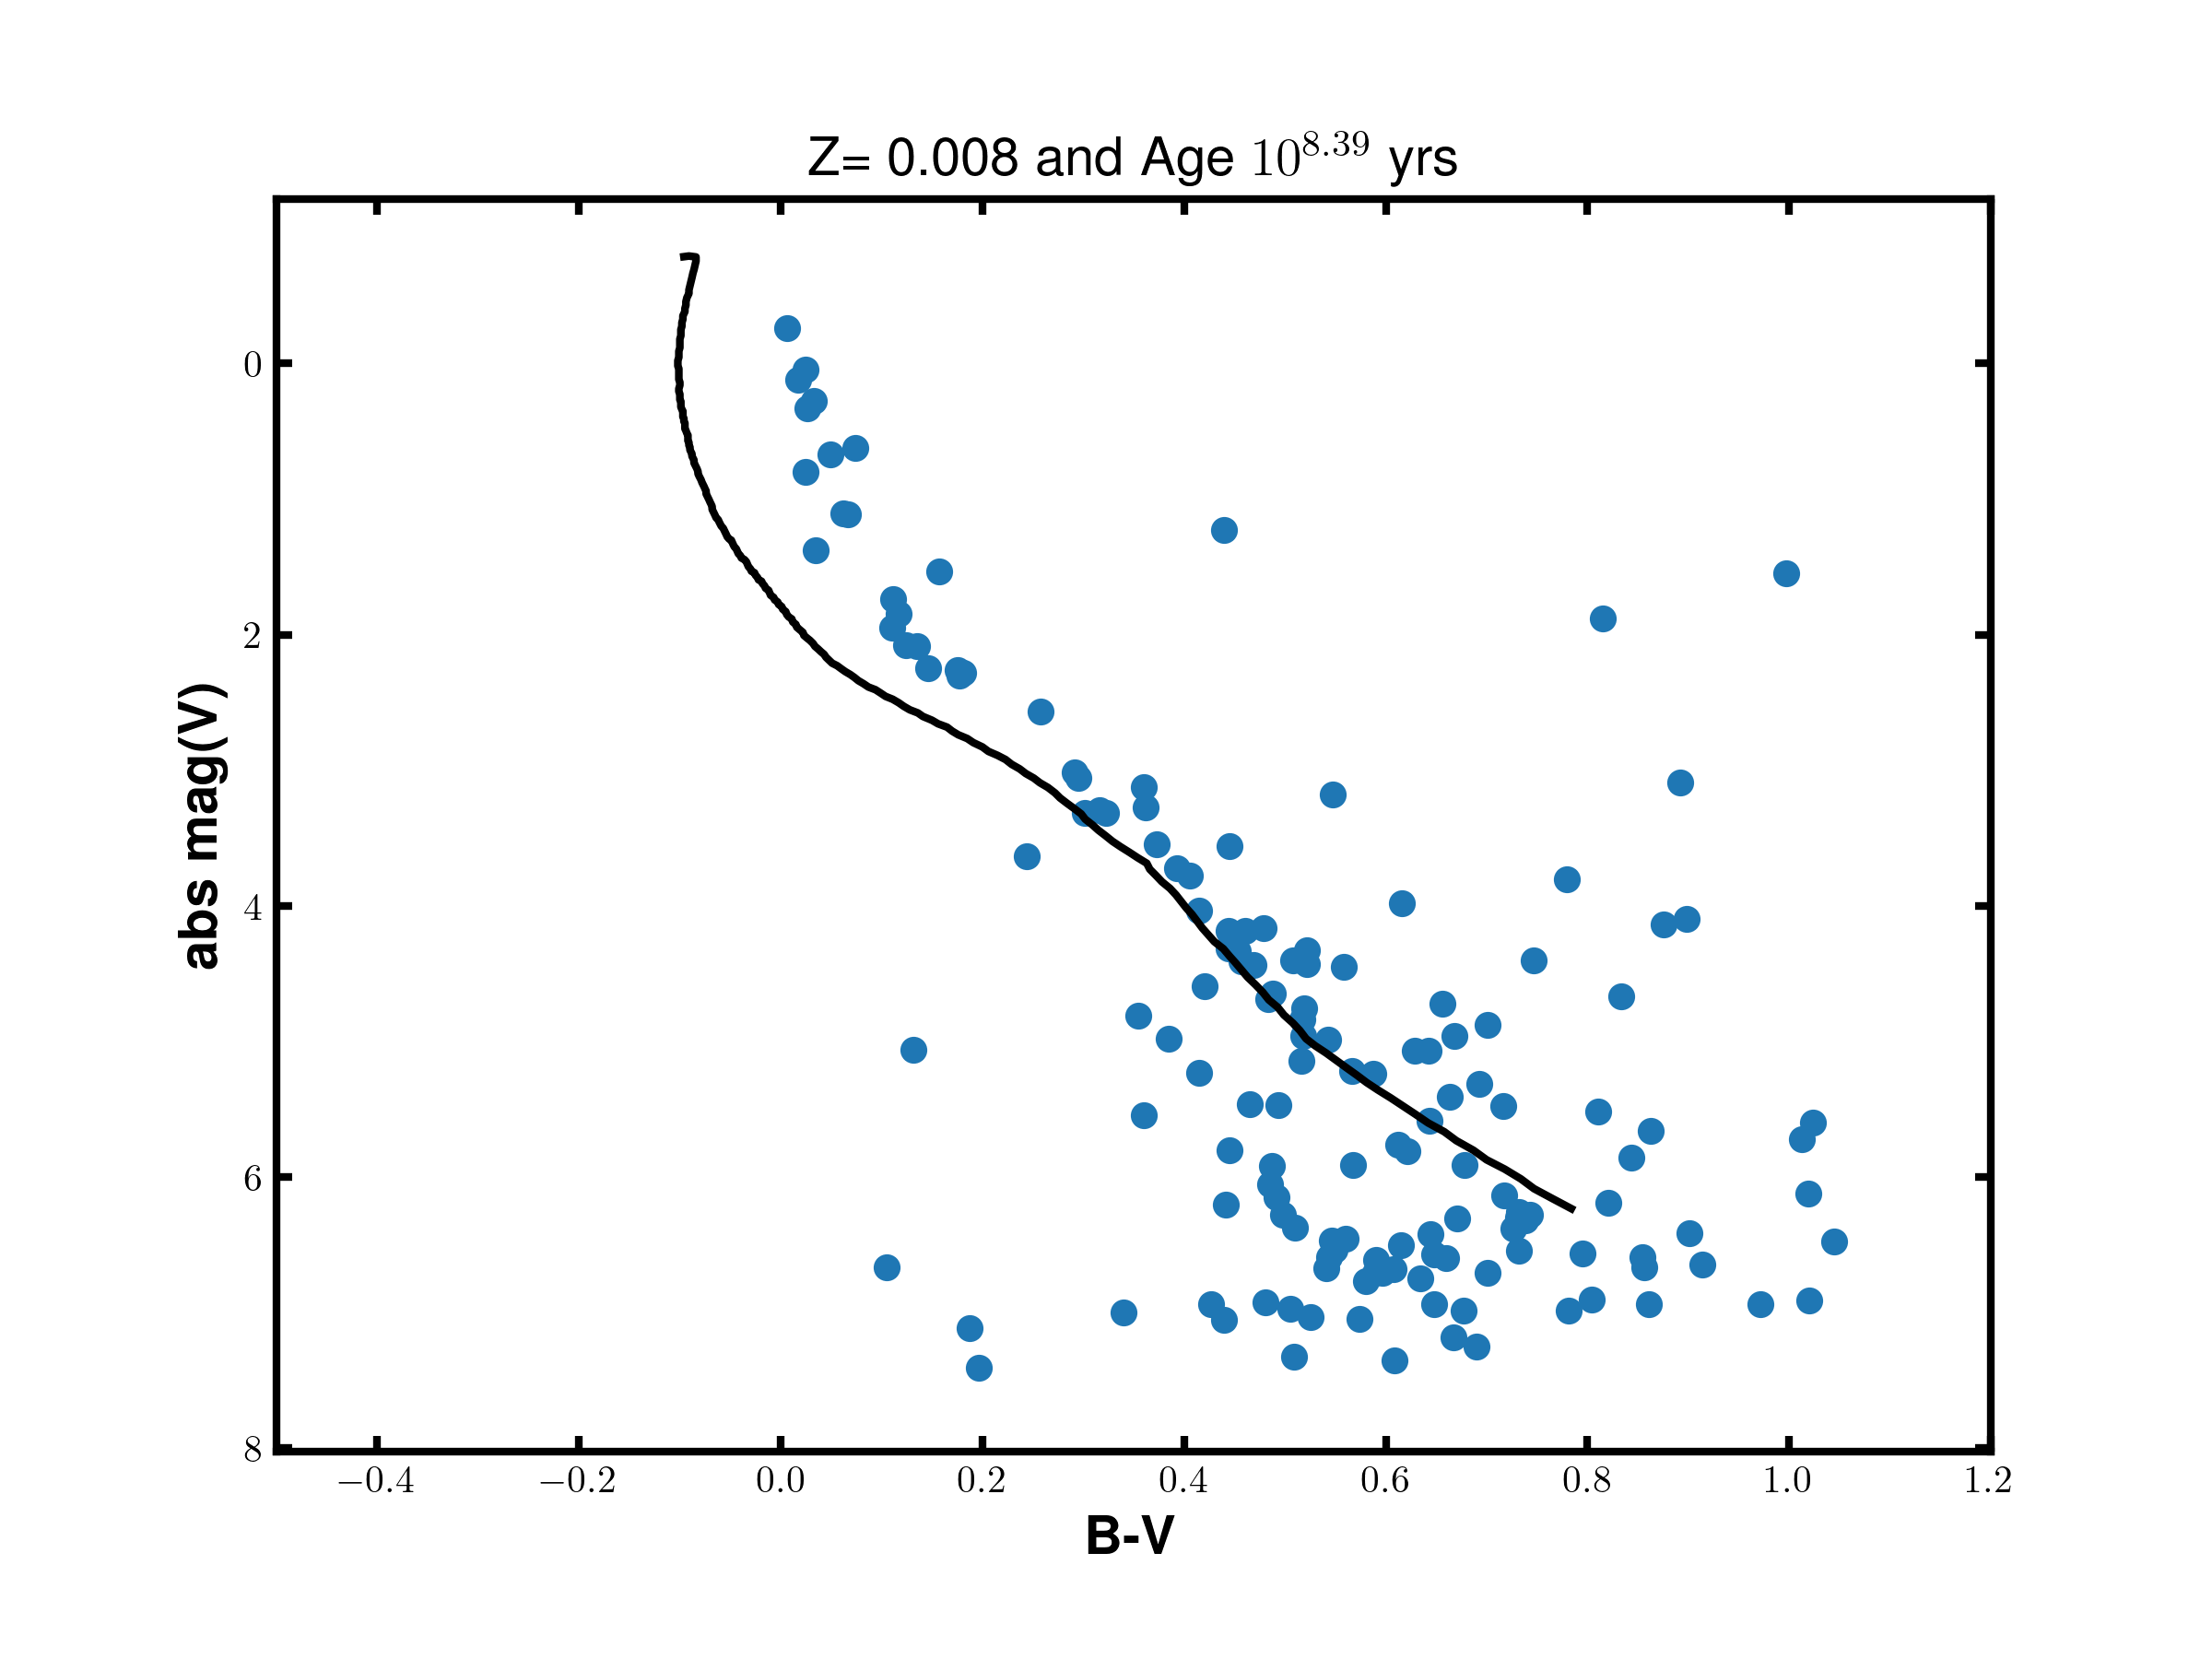
\includegraphics[width=\textwidth]{fig/iso_z008_839.png}
    \caption{CMD with an isochrone of z =0.008\& Age $10^{8.39}$}
    \end{figure}

    \begin{figure}[H]
    \centering
    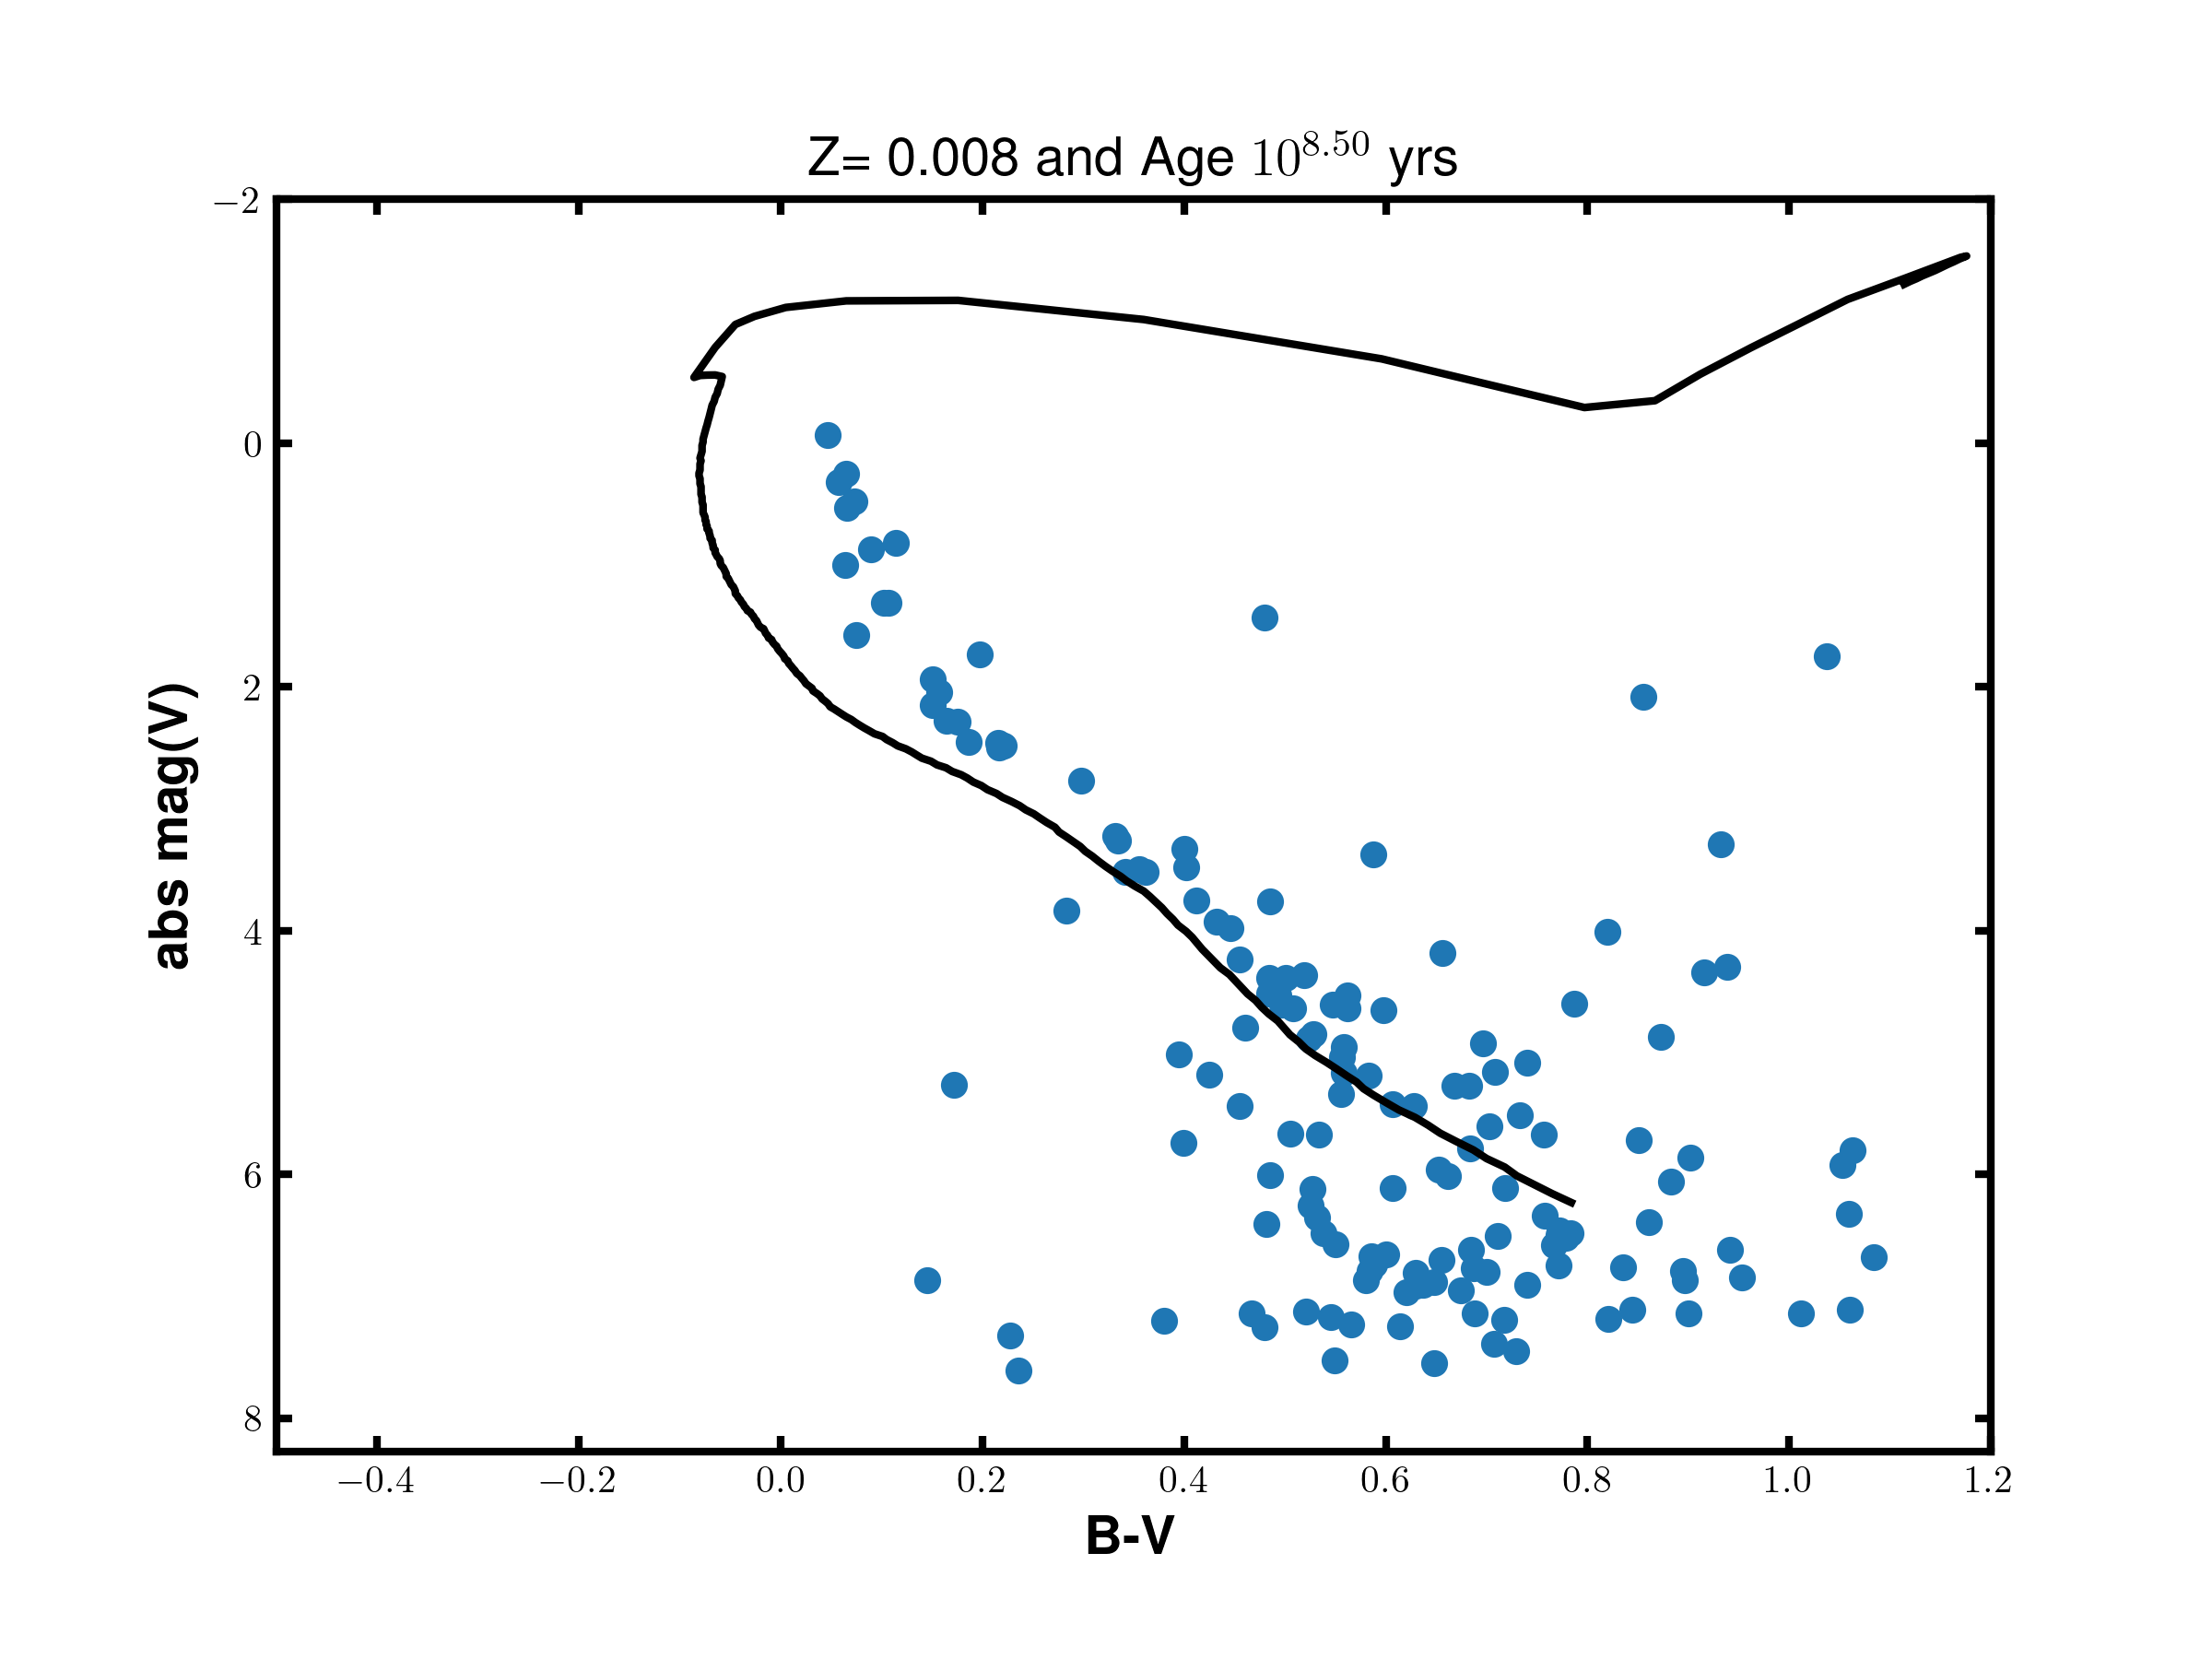
\includegraphics[width=\textwidth]{fig/iso_z008_850.png}
    \caption{CMD with an isochrone of z =0.008\& Age $10^{8.5}$}
    \end{figure}
    
    \begin{figure}[H]
    \centering
    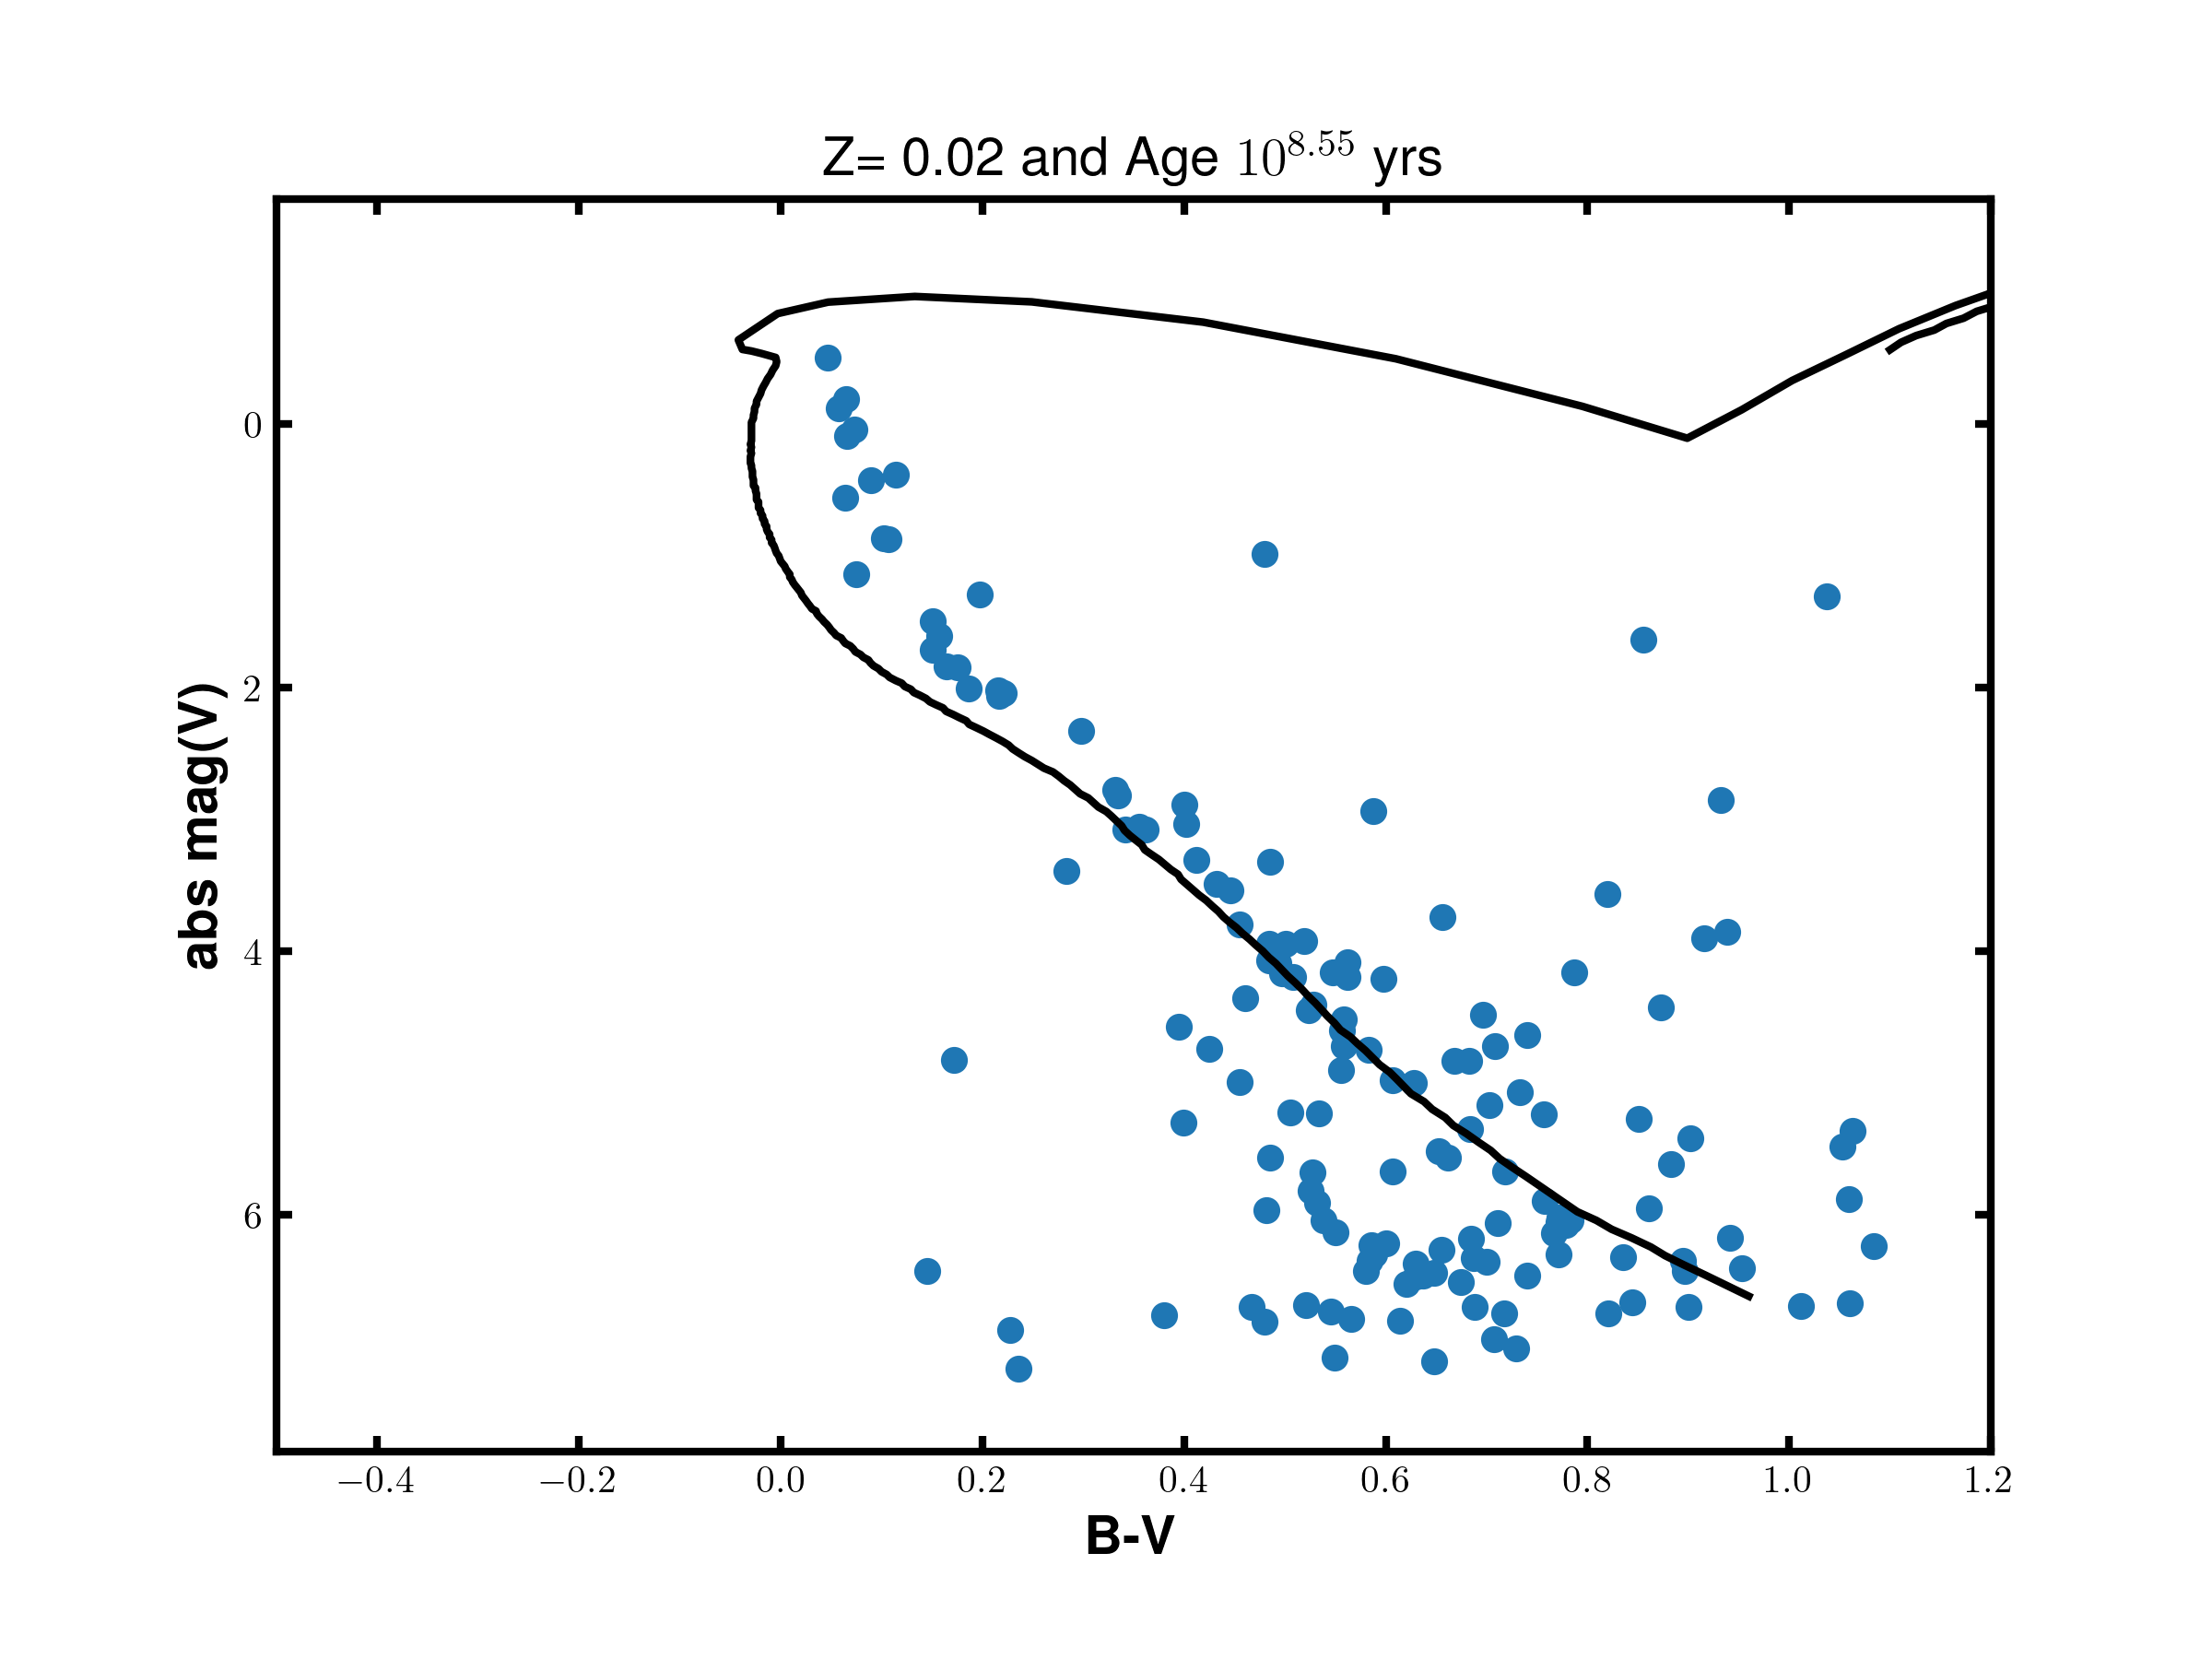
\includegraphics[width=\textwidth]{fig/iso_z020_855.png}
    \caption{CMD with an isochrone of z =0.02\& Age $10^{8.55}$}
    \end{figure}

    \begin{figure}[H]
    \centering
    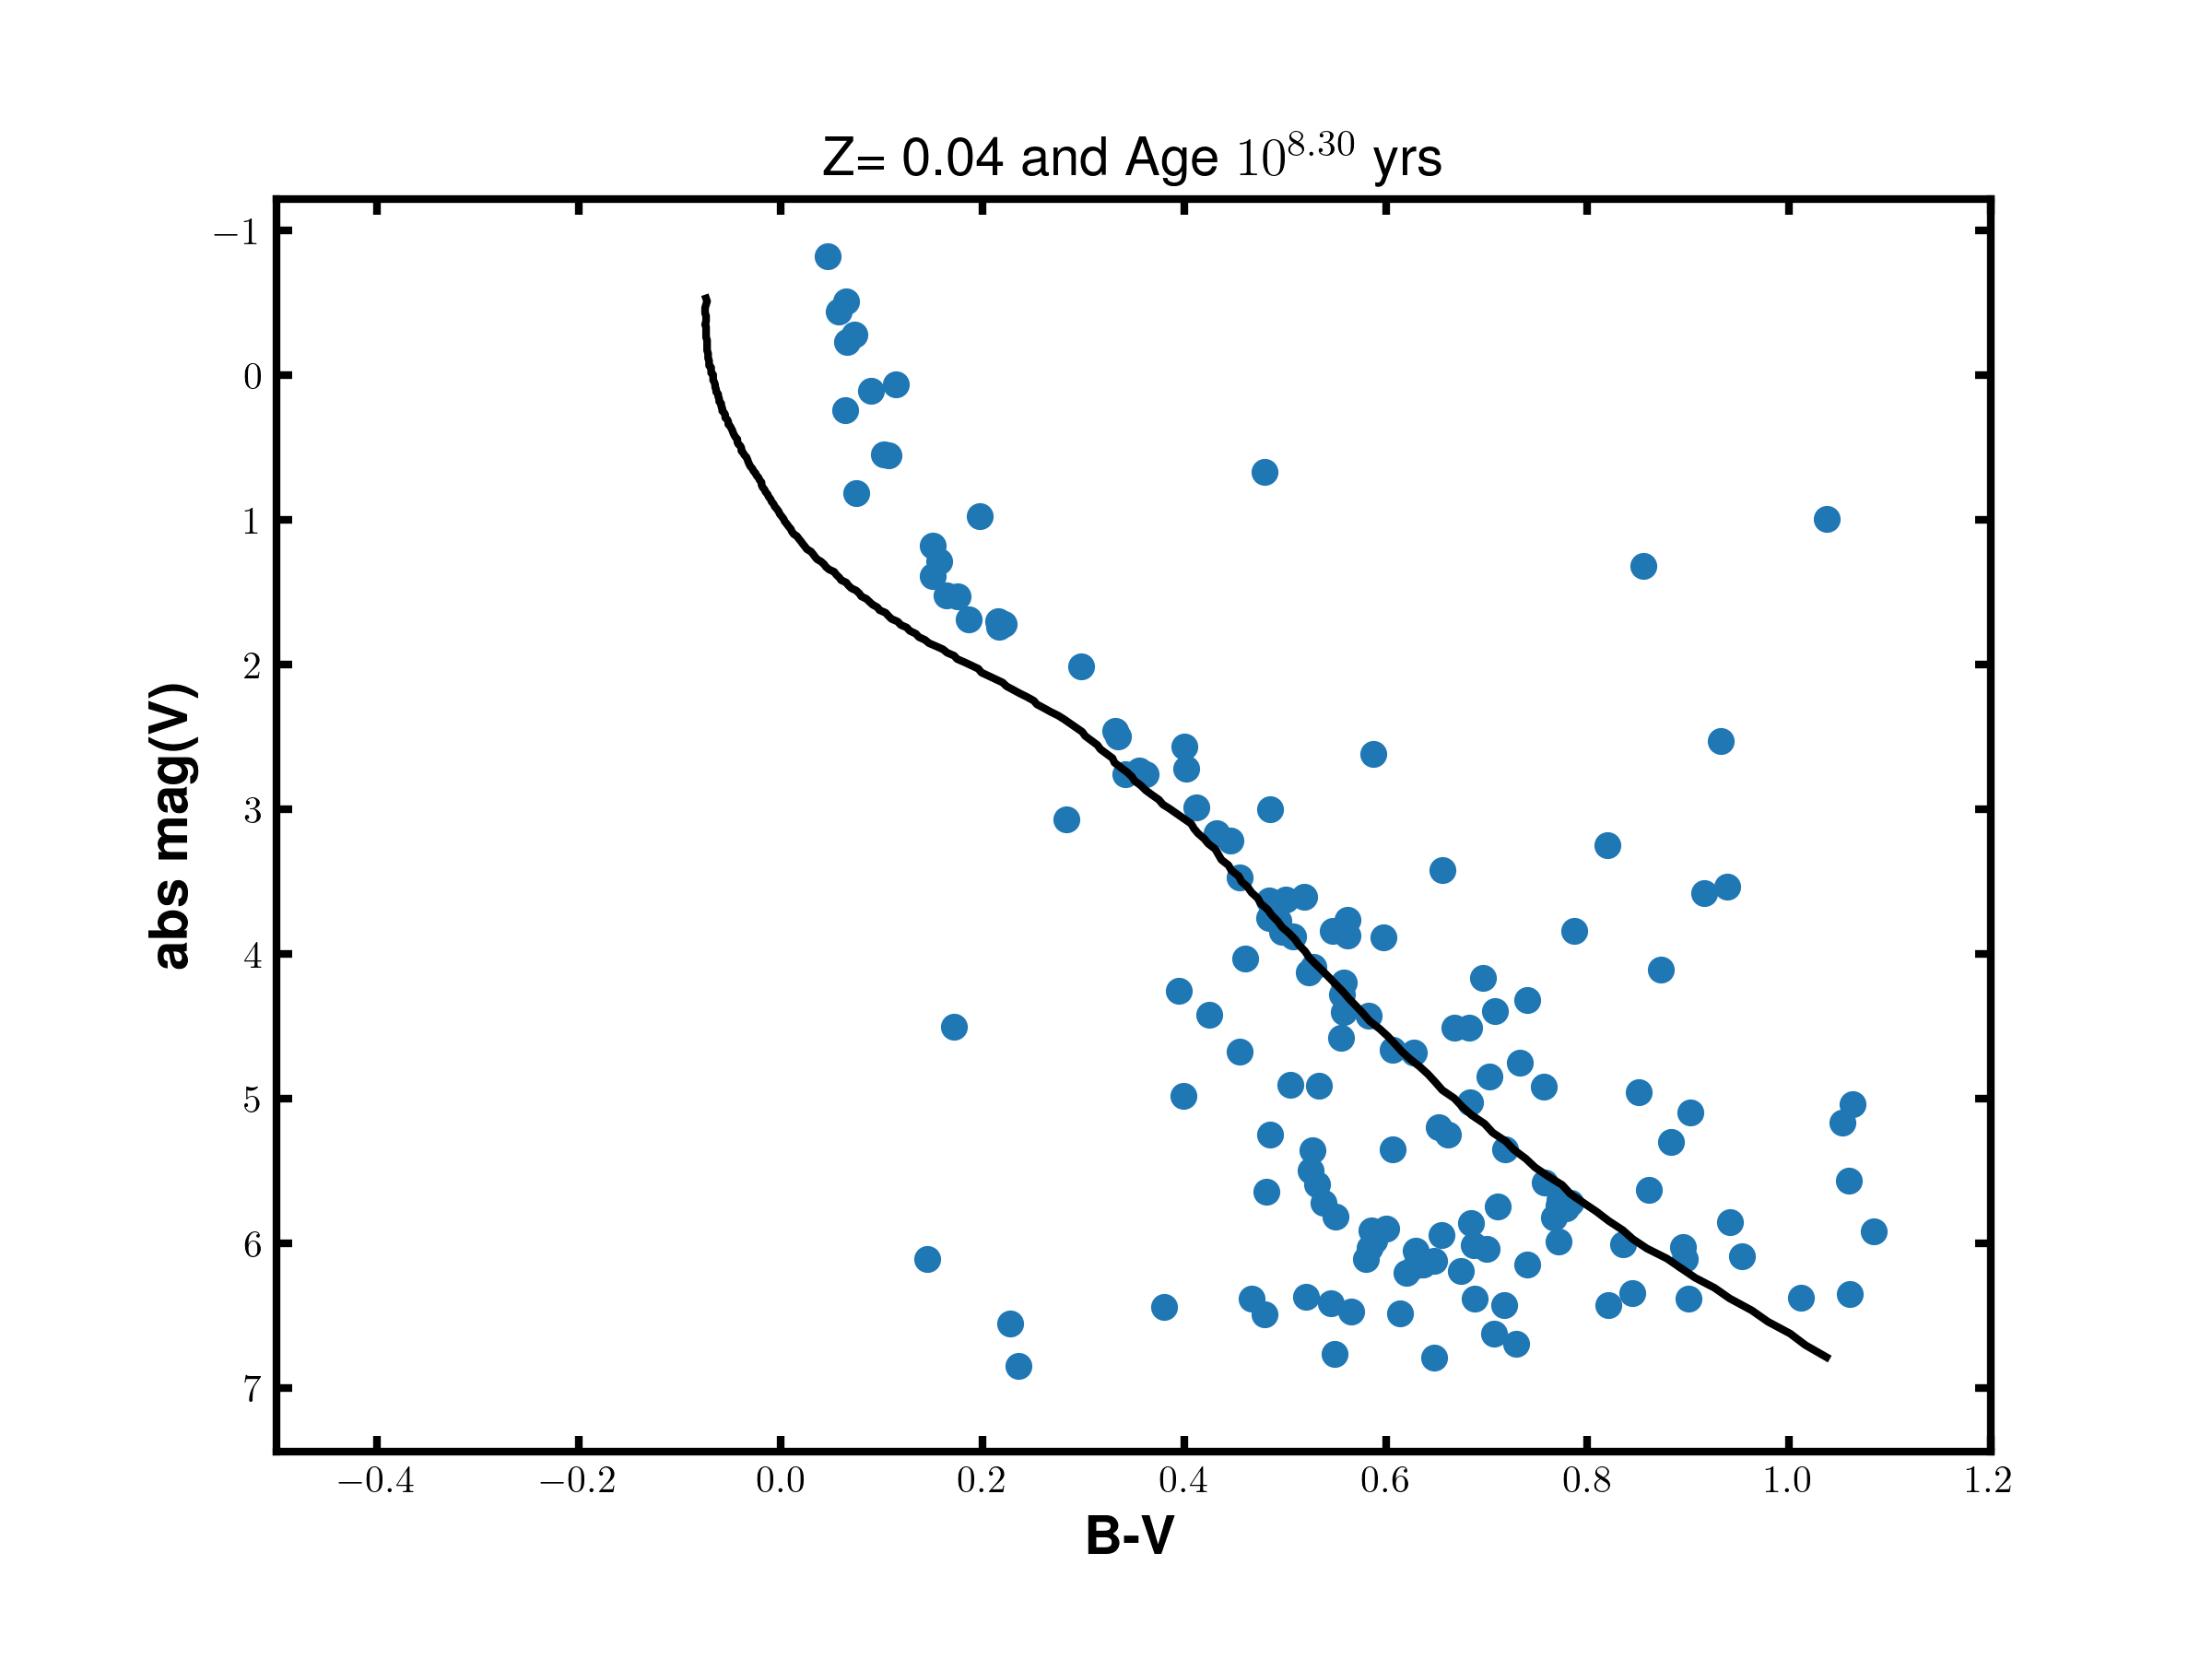
\includegraphics[width=\textwidth]{fig/iso_z040_830.png}
    \caption{CMD with an isochrone of z =0.04\& Age $10^{8.3}$}
    \end{figure}
    
    \begin{figure}[H]
    \centering
    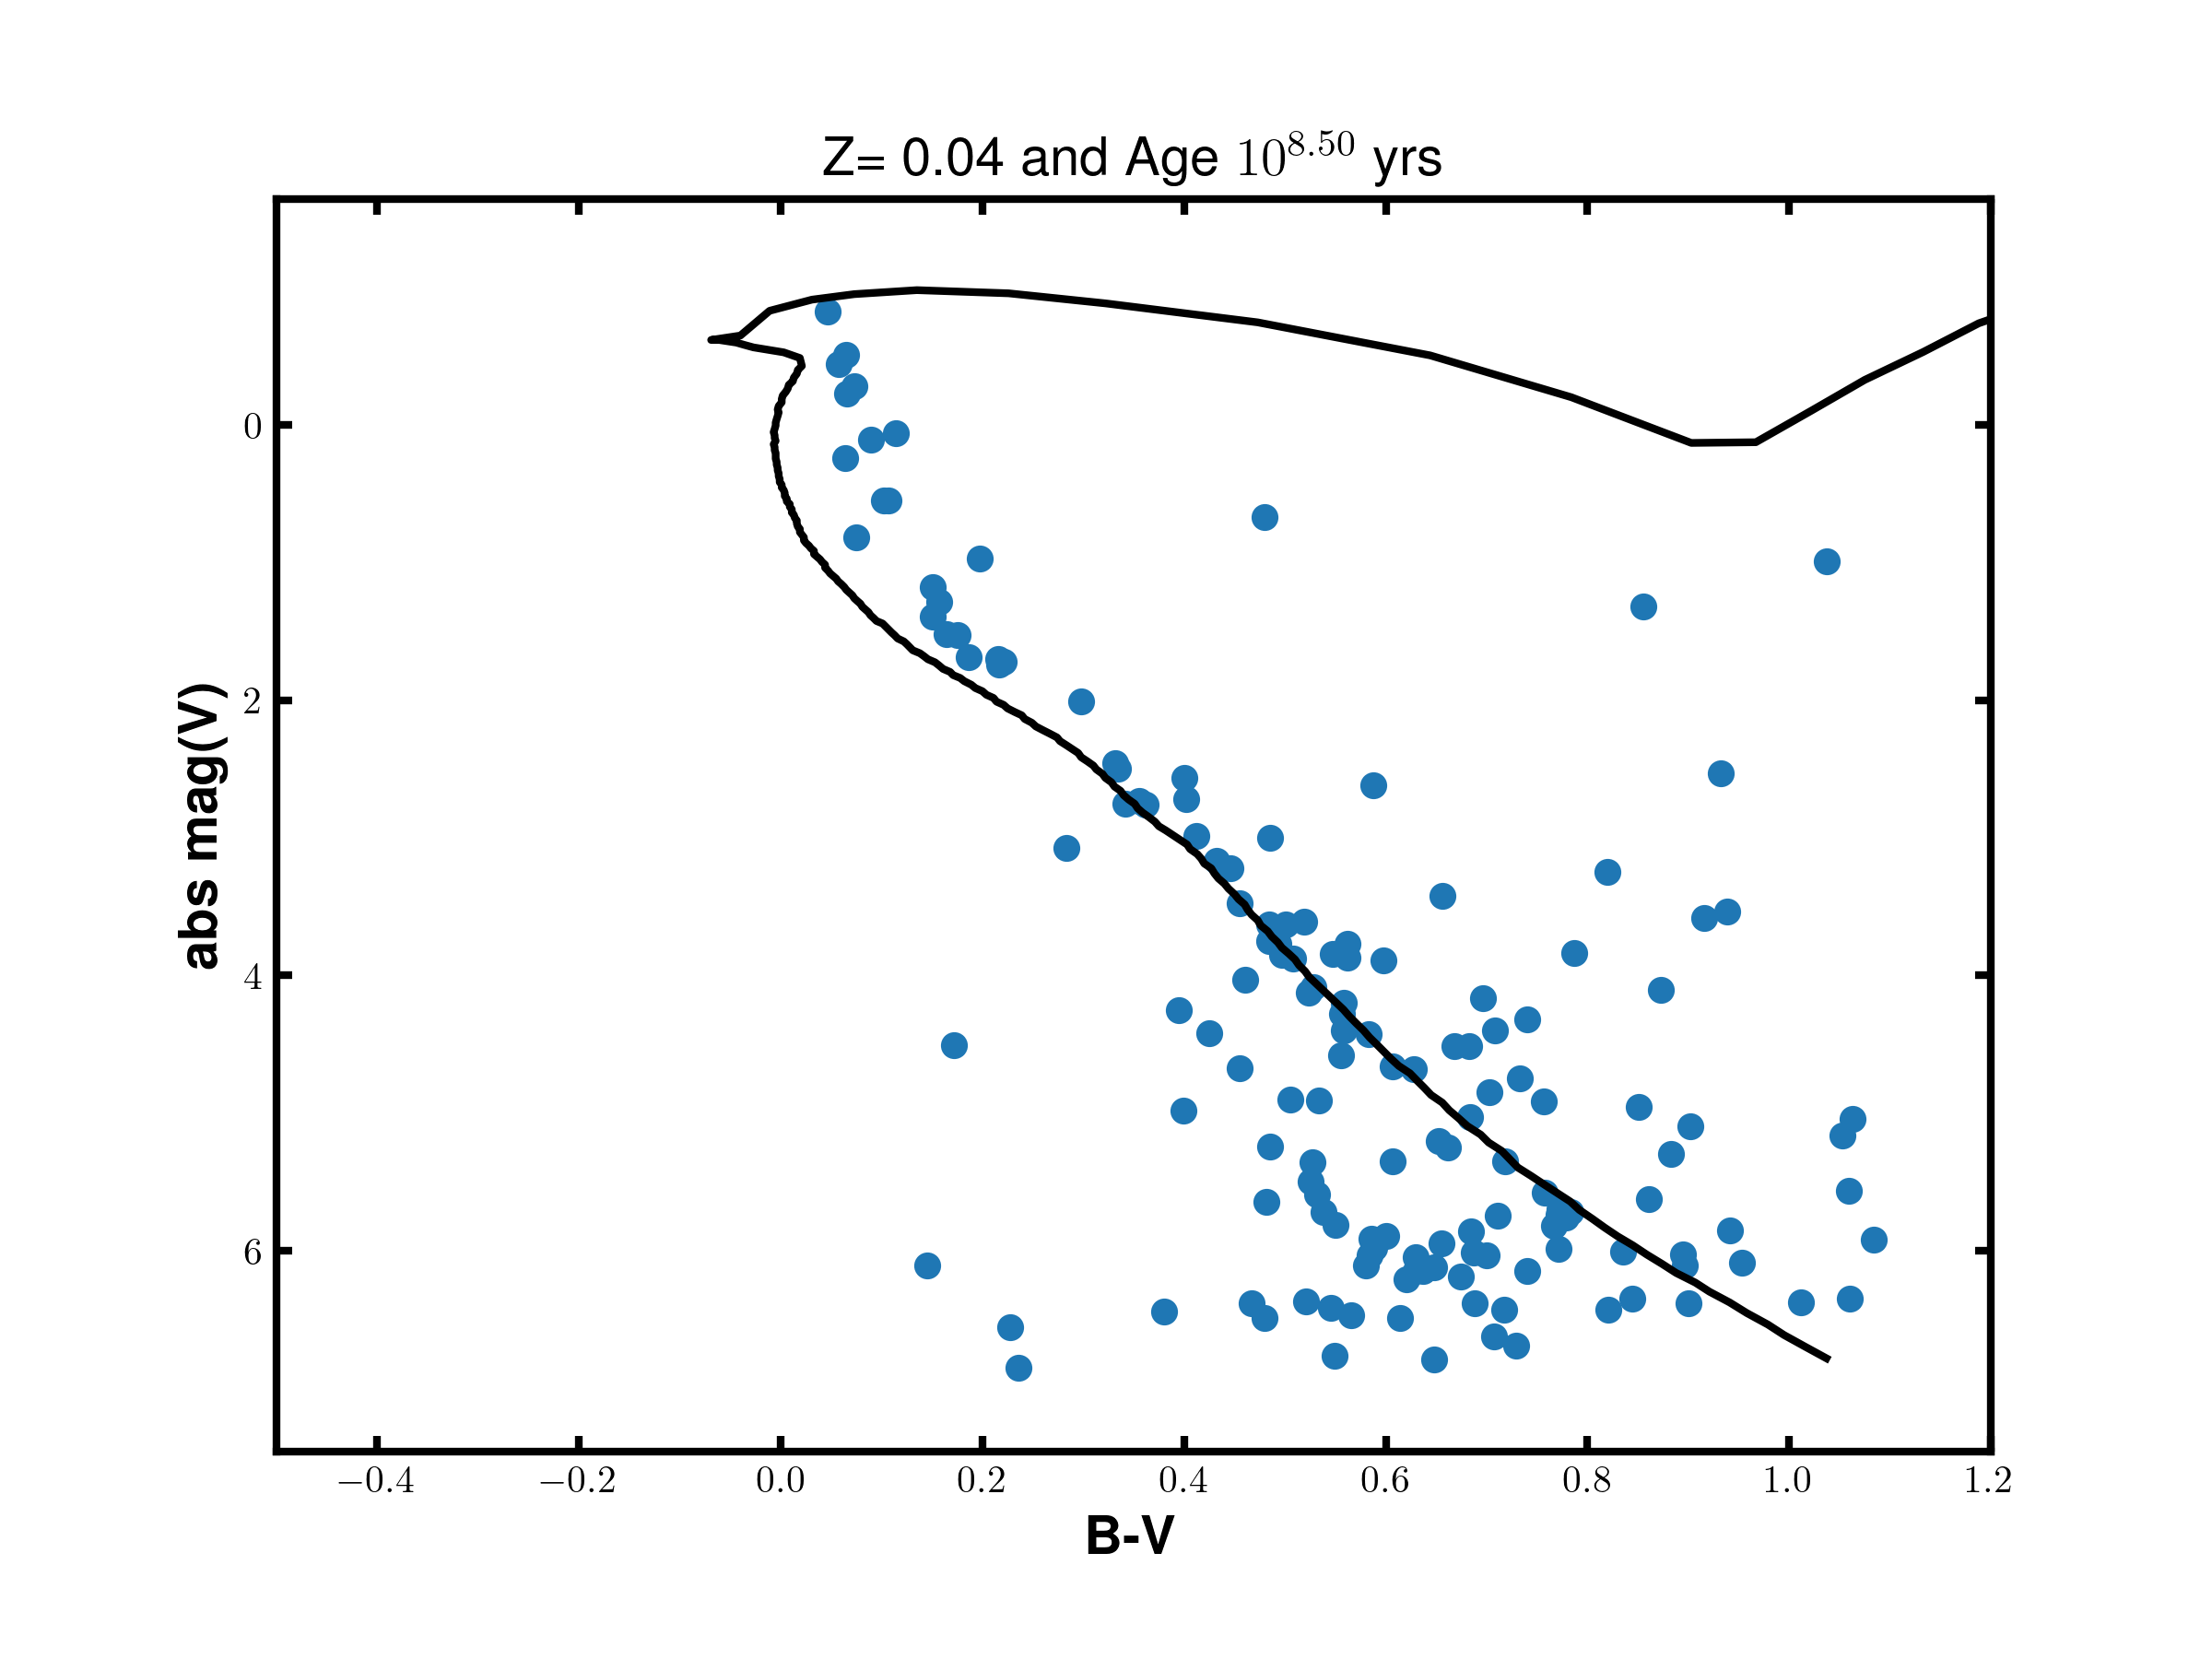
\includegraphics[width=\textwidth]{fig/iso_z040_850.png}
    \caption{CMD with an isochrone of z =0.04 \& Age $10^{8.5}$}
    \end{figure}
            
\end{document}